% **************************************************
% Document Class Definition
% **************************************************
\documentclass[
	paper=A4,					% paper size --> A4 is default in Germany
	twoside,					% onesite or twoside printing
	openright,					% doublepage cleaning ends up right side
	parskip=full,				% spacing value / method for paragraphs
	chapterprefix=true,			% prefix for chapter marks
	11pt,						% font size
	headings=normal,			% size of headings
	bibliography=totoc,			% include bib in toc
	listof=totoc,				% include listof entries in toc
	titlepage=on,				% own page for each title page
	captions=tableabove,		% display table captions above the float env
	draft=false,				% value for draft version
]{scrreprt}

\setcounter{tocdepth}{5}
\setcounter{secnumdepth}{5}

% **************************************************
% Debug LaTeX Information
% **************************************************
%\listfiles
\usepackage[utf8]{inputenc}
\usepackage[T1]{fontenc}
% **************************************************
% Information and Commands for Reuse
% **************************************************
\newcommand{\thesisTitle}{Análisis computacional del microbioma humano como fuente de biomarcadores clínicos}
\newcommand{\thesisAuthor}{Diego Fernández Edreira}
\newcommand{\thesisAuthorId}{48112826-T}
\newcommand{\thesisSubject}{Tesis Doctoral UDC / 2025}

\newcommand{\thesisDate}{Octubre 2025}
\newcommand{\thesisFullDate}{22~\thesisDate}
\newcommand{\thesisVersion}{Final version}

\newcommand{\thesisFirstSupervisor}{Dr. Carlos Fernández Lozano}
\newcommand{\thesisFirstSupervisorTitle}{Dr.}

\newcommand{\thesisSecondSupervisor}{Dr. Jose Liñares Blanco}
\newcommand{\thesisSecondSupervisorTitle}{Dr.}

\newcommand{\thesisUniversity}{Universidade da Coruña}

\newcommand{\thesisUniversityPhDProgramme}{Programa de doctorado en Tecnologías de la Información y las Comunicaciones}


\newcommand{\forceTitleIndent}{\leavevmode{\parindent=2.0em\indent}}
\newcommand{\forceUdcIndent}{\leavevmode{\parindent=5.0em\indent}}
\newcommand{\forceIndent}{\leavevmode{\parindent=1.5em\indent}}

% **************************************************
% Load and Configure Packages
% **************************************************
\usepackage[linesnumbered]{algorithm2e} 
\usepackage[utf8]{inputenc}		% defines file's character encoding
\usepackage[spanish]{babel}		% babel system, adjust the language of the content
\usepackage{lettrine}
\usepackage[					% clean thesis style
	figuresep=colon,%
	sansserif=false,%
	hangfigurecaption=false,%
	hangsection=true,%
	hangsubsection=true,%
	colorize=full,%
	colortheme=udc,%
	bibsys=bibtex,%
%	bibfile=bibliography,%
	bibstyle=numeric,%
]{cleanthesis}

\usepackage{xcolor,colortbl} % (fcedron) to set background color on cells

% listing  (fcedron)
\usepackage{listings}
\definecolor{mygreen}{rgb}{0,0.6,0}
\definecolor{mygray}{rgb}{0.5,0.5,0.5}
\definecolor{mymauve}{rgb}{0.58,0,0.82}

% v1 colors
%\definecolor{best_bg}{RGB}{218,244,223} %fcedron
%\definecolor{best_font}{RGB}{100,105,100} %fcedron
%\definecolor{worst_bg}{RGB}{255,218,223} %fcedron
%\definecolor{worst_font}{RGB}{192,100,104} %fcedron

% v2 colors
\definecolor{best_bg}{RGB}{198,239,206} %fcedron
\definecolor{best_font}{RGB}{0,97,41} %fcedron
\definecolor{worst_bg}{RGB}{255,199,206} %fcedron
\definecolor{worst_font}{RGB}{156,1,44} %fcedron

\newcommand{\bestRnga}[1]{\cellcolor{best_bg}\textbf{#1}}
\newcommand{\winRnga}[1]{\cellcolor{best_bg}\textcolor{best_font}{#1}}
\newcommand{\loseRnga}[1]{\cellcolor{worst_bg}\textcolor{worst_font}{#1}}

% for the best/worst column
\newcommand{\bwinRnga}[1]{\textcolor{best_font}{#1}}
\newcommand{\bloseRnga}[1]{\textcolor{worst_font}{#1}}

\lstset{ 
  backgroundcolor=\color{white},   % choose the background color; you must add \usepackage{color} or \usepackage{xcolor}; should come as last argument
  basicstyle=\footnotesize,        % the size of the fonts that are used for the code
  breakatwhitespace=false,         % sets if automatic breaks should only happen at whitespace
  breaklines=true,                 % sets automatic line breaking
  captionpos=b,                    % sets the caption-position to bottom
  commentstyle=\color{mygreen},    % comment style
  frame=single,	                   % adds a frame around the code
  keepspaces=true,                 % keeps spaces in text, useful for keeping indentation of code (possibly needs columns=flexible)
  keywordstyle=\color{blue},       % keyword style
  morekeywords={*,...},            % if you want to add more keywords to the set
  numbers=left,                    % where to put the line-numbers; possible values are (none, left, right)
  numbersep=5pt,                   % how far the line-numbers are from the code
  numberstyle=\tiny\color{mygray}, % the style that is used for the line-numbers
  rulecolor=\color{black},         % if not set, the frame-color may be changed on line-breaks within not-black text (e.g. comments (green here))
  showspaces=false,                % show spaces everywhere adding particular underscores; it overrides 'showstringspaces'
  showstringspaces=false,          % underline spaces within strings only
  showtabs=false,                  % show tabs within strings adding particular underscores
  stepnumber=2,                    % the step between two line-numbers. If it's 1, each line will be numbered
  stringstyle=\color{mymauve},     % string literal style
  tabsize=2,	                   % sets default tabsize to 2 spaces
  title=\lstname                   % show the filename of files included with \lstinputlisting; also try caption instead of title
}

\hypersetup{					% setup the hyperref-package options
	pdftitle={\thesisTitle},	% 	- title (PDF meta)
	pdfsubject={\thesisSubject},% 	- subject (PDF meta)
	pdfauthor={\thesisAuthor},	% 	- author (PDF meta)
	plainpages=false,			% 	-
	colorlinks=false,			% 	- colorize links?
	pdfborder={0 0 0},			% 	-
	breaklinks=true,			% 	- allow line break inside links
	bookmarksnumbered=true,		%
	bookmarksopen=true			%
}

% **************************************************
% BIBLIOGRAPHY
% **************************************************

\bibliography{bibliography}


%%%%%%%%%%%%%%%% My Own packages %%%%%%%%%%%%%%%%%%%%%%%%%%
% From CHC-RT paper
\usepackage{amsmath}
\usepackage{amsfonts} % (fcedron) for approach chapter
\usepackage{multirow}

% From SSVDAG paper
\usepackage{longtable}
\usepackage{xhfill}
\newcommand{\ditto}{\textquotedbl~~~}
\usepackage[normalem]{ulem}
\usepackage{enumitem}
\usepackage{setspace}
\usepackage{microtype}
\usepackage{listings}
\usepackage{subfig}

%%%%%%%%%%%%%%%%%%%%% Misc stuff %%%%%%%%%%%%%%%%%%%%%%%%%%%
\usepackage{changepage}

\usepackage{datetime}
\usepackage[xindy]{glossaries}
\usepackage{graphbox}
\usepackage{caption}
\usepackage{multicol}
\usepackage{makecell}
\usepackage[titletoc, header]{appendix}
\usepackage{hyperref}

%% Add pdfs
\usepackage{pdfpages}


%%% removing warnings
\usepackage{csquotes}
\usepackage{scrhack}
\pdfminorversion=6

\definecolor{udcColor}{RGB}{206,0,130}
\definecolor{grayColor}{RGB}{186,186,186}
\definecolor{FIXMEColor}{rgb}{1,0,0}
\newcommand{\FIXME}[1]{{\color{FIXMEColor}{\textbf{FIXME: #1}}}}

\newcommand{\chapterintro}[1]{	
	\begingroup
	\vspace{-5pt}
	\leftskip3.2em
	\rightskip\leftskip
	\setstretch{1.1} \sffamily \small #1
	\vspace{5pt}
	\par
	\endgroup
}


% **************************************************
% Document CONTENT
% **************************************************
\begin{document}

% --------------------------
% rename document parts
% --------------------------
\renewcaptionname{spanish}{\figurename}{Fig.}
\renewcaptionname{spanish}{\tablename}{Tab.}
\renewcommand{\lstlistingname}{Lis.}
\renewcommand{\chaptername}{Capítulo}
\renewcommand{\contentsname}{Tabla de contenidos}
\renewcommand{\listtablename}{Índice de tablas}
\renewcommand{\listfigurename}{Índice de figuras}
\renewcommand{\bibname}{Referencias}
\renewcommand{\appendixname}{Anexo}


% --------------------------
% Front matter
% --------------------------
\pagenumbering{roman}			% roman page numbing (invisible for empty page style)

\pagestyle{empty}				% no header or footers
%
%   TITLE PAGES - COVERS
%

%%%%%%%%%%% MAIN COVER %%%%%%%%%%%%

\newgeometry{margin=1in}
\begin{titlepage}
	\pdfbookmark[0]{Title and front pages}{Title and front pages}
	\label{front:titlepage}
	\tgherosfont


	\vspace*{30pt}


	{\huge  
	\begin{spacing}{1.15}
	\forceTitleIndent	
		\thesisTitle 
		\end{spacing}
		}
	
	
	\vspace*{40pt}
	
\begin{spacing}{0}
	{\Large \thesisAuthor} 

	\textcolor{udcColor}{\noindent\rule[-3.5ex]{\textwidth}{3pt}}
	\textcolor{grayColor}{\noindent\rule{\textwidth}{2.5pt}}
	\textcolor{udcColor}{\noindent\rule[3.5ex]{\textwidth}{3pt}}
	{\large \thesisSubject} \\[0.001mm]	
\end{spacing}	

	\vspace*{80pt}

    \textsf{\textbf{Directores:}} \\
	\textsf{ \thesisFirstSupervisor} \\
	\textsf{ \thesisSecondSupervisor}



	\vspace*{120pt}

{ \centering
	\textsf{\thesisUniversityPhDProgramme} \\	
	\vspace*{40pt}
	
\includegraphics[width=7.25cm]{img/udc} \\[1mm]
}

%	\begin{flushright}
%	\scriptsize
%	\textbf{Version}: \thesisVersion \\[0mm]
%	\textbf{Compilation}: \today\ at \currenttime
%	\end{flushright}
\end{titlepage}
\restoregeometry
		% INCLUDE: all titlepages
\cleardoublepage

\titlespacing*{\chapter}{0pt}{0pt}{0pt} % change the gap around the chapter name

\pagestyle{plain}				% display just page numbers

%
%   CERTIFICATION OF COMPLIANCE  
%
%%%%%%%%% TODO %%%%%%%%%%
% - Check everything Ok
% - Check translation

\label{front:declaration_compilance}
\clearpage

\begin{spacing}{0}
	\color{udcColor}
	\forceUdcIndent \textit{Escola Internacional de Doutoramento}\\
	\forceUdcIndent \textit{Vicerreitoría de Investigación e Transferencia} \\
	
\includegraphics[width=7.25cm]{img/udc} \\[1mm]
\end{spacing}

\vspace*{30pt}	

% \thesisFirstSupervisorTitle~
% \thesisSecondSupervisorTitle~
\begin{center}
\begin{tabular}{ p{6.5cm}p{0.5cm}p{6.5cm} }
	\textbf{\thesisFirstSupervisor},  Profesor Titular del área de Ciencias de la Computación e Inteligencia Artificial de la \thesisUniversity.
	& & 
	\textbf{\thesisSecondSupervisor}, investigador postdoctoral en el Instituto Europeo de Bioinformática del EMBL, Hixton.
\end{tabular}
\end{center}
	
\vspace*{30pt}

\textbf{HACEN CONSTAR QUE:}

\forceIndent La Tesis Doctoral titulada \textbf{Análisis computacional del microbioma humano como fuente de biomarcadores clínicos}, realizada por D. \thesisAuthor~ con el número de identidad \thesisAuthorId, bajo nuestra dirección en el Departamento de Ciencias de la Computación y Tecnologías de la Información, cumple los requisitos para optar al grado de Doctor.


\vspace*{30pt}

Y para que así conste, firman esta autorización en A Coruña, a \thesisFullDate

\vspace*{30pt}

Los directores de la Tesis Doctoral

\begin{center}
	\begin{tabular}{ c p{1.5cm} c} 
		\\
		Fdo. \thesisFirstSupervisor
		 & &
		Fdo. \thesisSecondSupervisor
	\end{tabular}
\end{center}


\cleardoublepage

%
%   DEDICATION
%
\label{sec:dedication}

\begin{flushright}
    \thispagestyle{empty}

        \textbf{{A mi familia:}}\\

    \textit{el faro en la niebla,} \\
    \textit{el ancla en la borrasca}\\
    \textit{y el puerto al que regresar.}\\
\end{flushright}

\cleardoublepage

%
%   Acknowkegments
%

\pdfbookmark[0]{Acknowledgements}{Acknowledgements}
\chapter*{Agradecimientos}
\label{front:acknowledgments}


{\textsc
Gracias por acogerme con ilusión y respeto. Gracias por guiarme y aconsejarme tan bien durante estos años, no solo en lo profesional. Agradezco vuestra comprensión a lo largo de los obstáculos que han surgido en esta etapa. Pero, sobre todo, gracias por vuestra sinceridad y honestidad en todo momento. Intentaré seguir trabajando de acuerdo con los pilares que habéis estado cimentando estos años. Gracias Carlos. Gracias Jose.

\vspace{-8pt}

Gracias al grupo RNASA por haberme dado una oportunidad en primera instancia. Gracias a todos los miembros del grupo que me han apoyado desde mi llegada y después de mi partida. En especial a Andrés, Alex, Rubén y Brais. Mira que hemos \textit{esbardallado} en esas cuatro paredes. Esos cafés, cenas y cervezas han sido gasolina en los momentos de flaqueza. Gracias por estar empujando desde el inicio.

\vspace{-8pt}

Gracias a la gente del MALL. Ese soplo de aire fresco necesario para finalizar esta etapa de mi vida y abrir un nuevo camino. Este último año ha sido complicado, pero he podido contar con vosotros. Lucía, Samuel, siento deciros que se vienen más \textit{cuncas}. Gracias chicos.

\vspace{-8pt}

Gracias a mi familia por absolutamente todo. Si no fuera por vosotros, no sé qué habría sido de mí. A pesar de no entender del todo lo que hago o a qué me dedico, me habéis apoyado incondicionalmente en todo momento. Mamá, gracias por aguantarme en los buenos, pero sobre todo en los malos momentos. Gracias por estar ahí, aunque choquemos continuamente. Carla, gracias por ser un pilar indiscutible en este viaje; espero seguir compartiendo logros contigo. Me siento eternamente agradecido de teneros en mi vida.

\vspace{-8pt}

Gracias a la familia que se elige: \textit{Fueguitos}, Bruno, Dova. Ojalá haber estado más presente en vuestras vidas estos últimos años. Gracias por ayudarme e impulsarme a crecer. Gracias por ser esa válvula de escape y ese apoyo incondicional.

\vspace{-8pt}

A todos vosotros, \textit{graciñas}.

\vspace{-8pt}


}
\cleardoublepage


\label{sec:quote}
\clearpage
\begin{center}
\thispagestyle{empty}

\vspace*{20pt}

	\cleanchapterquote{We leave traces of ourselves wherever we go, on whatever we touch.} {Lewis Thomas}


\end{center}


\cleardoublepage

%
%   ABSTRACTS
%

\pdfbookmark[0]{Abstracts}{Abstracts}



%%%%%%%%%% Castellano %%%%%%%%%%%%
                                                                   
\pdfbookmark[1]{Resumen (Spanish abstract)}{Resumo (Spanish abstract)}
\chapter*{Resumen}
\markboth{\color[cmyk]{.0, 1.00, .37, .19} Resumen (thesis abstract in Spanish)}{}
\markright{\color[cmyk]{.0, 1.00, .37, .19} Resumen (thesis abstract in Spanish)}{}
\label{sec:abstract_spanish}

El estudio del microbioma humano ha avanzado de forma acelerada gracias a la caída del coste de la secuenciación y a la disponibilidad de grandes repositorios públicos. Este progreso ha confirmado asociaciones entre perfiles microbianos y múltiples patologías, pero también ha puesto de relieve retos persistentes: la naturaleza composicional de los datos procedentes del microbioma, el ruido técnico y la variabilidad interindividual. En este contexto, los enfoques de \textit{Machine Learning} brindan una ventaja sustancial para detectar señales complejas con posible significado biológico y estimar con rigor el valor predictivo de los perfiles microbianos en entornos clínicos. 

Esta Tesis Doctoral responde a dichos desafíos adoptando un enfoque computacional estandarizado y reproducible, desde el procesado de lecturas 16S rRNA hasta la aplicación de modelos de \textit{Machine Learning} para el análisis de estos datos. Bajo este enfoque computacional, se identifican patrones microbianos que distinguen de forma consistente distintos estados clínicos en enfermedades metabólicas (síndrome metabólico y diabetes tipo 2); se obtienen modelos predictivos para diabetes tipo 1 sustentados en un conjunto acotado de taxones con alta relevancia biológica; y, en vaginosis bacteriana, se propone un subtipado alternativo del microbioma vaginal que añade información complementaria no recogida por otros métodos de estratificación, y puede apoyar la predicción de la respuesta terapéutica. Estos resultados se presentan en un compendio de tres publicaciones científicas. 

En conjunto, esta Tesis Doctoral ofrece evidencia de que los perfiles microbianos permiten la caracterización de estados clínicos y ofrece un marco metodológico reproducible que facilita su evaluación comparativa entre cohortes. 


%%%%%%%%%% Galego %%%%%%%%%%%%


\pdfbookmark[1]{Resumo (Galician abstract)}{Resumo (Galician abstract)}
\chapter*{Resumo}
\markboth{\color[cmyk]{.0, 1.00, .37, .19} Resumo (thesis abstract in Galician)}{}
\markright{\color[cmyk]{.0, 1.00, .37, .19} Resumo (thesis abstract in Galician)}{}
\label{sec:abstract_galician}

O estudo do microbioma humano avanzou de forma acelerada grazas á caída do custo da secuenciación e á dispoñibilidade de grandes repositorios públicos. Este progreso confirmou asociacións entre perfís microbianos e múltiples patoloxías, pero tamén puxo de relevo retos persistentes: a natureza composicional dos datos procedentes do microbioma, o ruído técnico e a variabilidade interindividual. Neste contexto, os enfoques de \textit{Machine Learning} brindan unha vantaxe substancial para detectar sinais complexos con posible significado biolóxico e estimar con rigor o valor preditivo dos perfís microbianos en escenarios clínicos.

Esta Tese Doutoral responde aos devanditos desafíos adoptando un enfoque computacional estandarizado e reproducible, desde o procesado de lecturas 16S rRNA ata a aplicación de modelos de \textit{Machine Learning} para a análise destes datos. Baixo este enfoque computacional, identifícanse patróns microbianos que distinguen de forma consistente distintos estados clínicos en enfermidades metabólicas (síndrome metabólico e diabetes tipo 2); obtéñense modelos preditivos para diabetes tipo 1 sustentados nun conxunto acoutado de taxóns con alta relevancia biolóxica; e, en vaxinose bacteriana, proponse un subtipado alternativo do microbioma vaxinal que engade información complementaria non recollida por outros métodos de estratificación, e pode apoiar a predición da resposta terapéutica. Estes resultados preséntanse nun compendio de tres publicacións científicas.

En conxunto, esta Tese Doutoral ofrece evidencia de que os perfís microbianos permiten a caracterización de estados clínicos e ofrece un marco metodolóxico reproducible que facilita a súa avaliación comparativa entre cohortes.			% Include Spanish and Galcian
\cleardoublepage

%%% Estructura de la tesis %%%
\pdfbookmark[0]{Structure}{Structure}
\chapter*{Estructura de la Tesis Doctoral}

Esta Tesis Doctoral está estructurada en seis secciones. El \textbf{Capítulo \ref{chap:introduction}} presenta una introducción del trabajo, dividida en dos secciones: Microbioma y Métodos y Técnicas Computacionales. La primera sección establece el marco biológico del estudio, mientras que la segunda sección introduce las herramientas y enfoques que se han empleado a lo largo de esta Tesis Doctoral. En el \textbf{Capítulo \ref{chap:objectives}} se enumeran los objetivos propuestos, los cuales han motivado la realización de esta Tesis Doctoral.

El \textbf{Capítulo \ref{chap:results}} expone los resultados obtenidos durante el desarrollo de la Tesis Doctoral. Este capítulo está dividido en tres secciones, las cuales se corresponden con los trabajos que conforman el compendio. En cada una de ellas se expone el contexto y los resultados obtenidos en cada uno de los trabajos. Además, se adjunta una copia de cada uno de ellos. Las referencias de los trabajos, por orden de aparición, son las siguientes:

\begin{my_list_item}
	
    \item Loaiza, L. I. S., \textbf{Fernández-Edreira, D.}, Liñares-Blanco, J., Cepeda, A., Cardelle-Cobas, A., and Fernandez-Lozano, C. (2025). Fecal microbiome analysis in patients with metabolic syndrome and type 2 diabetes. PeerJ, 13, e19108. Q2, 2.4 IF. 1 cita (Google Scholar). \url{https://doi.org/10.7717/peerj.19108}
    
    \item \textbf{Fernández-Edreira, D.}, Liñares-Blanco, J., and Fernandez-Lozano, C. (2021). Machine Learning analysis of the human infant gut microbiome identifies influential species in type 1 diabetes. Expert Systems with Applications, 185, 115648. Q1, 8.665 IF. 48 citas (Google Scholar). \url{https://doi.org/10.1016/j.eswa.2021.115648}
    
    \item \textbf{Fernández-Edreira, D.}, Liñares-Blanco, J., Patricia, V., and Fernandez-Lozano, C. (2024). VIBES: A consensus subtyping of the vaginal microbiota reveals novel classification criteria. Computational and Structural Biotechnology Journal, 23, 148-156. Q2, 4.1 IF. 4 citas (Google Scholar). \url{https://doi.org/10.1016/j.csbj.2023.11.050}
    
\end{my_list_item}

En el \textbf{Capítulo \ref{chap:discussion}}, se lleva a cabo una discusión integrada de los tres trabajos realizados, resaltando los puntos comunes que fueron esenciales en su desarrollo y brindando coherencia, cohesión y justificación al trabajo de investigación en su conjunto. El \textbf{Capítulo \ref{chap:conclussions}} enumera las conclusiones obtenidas a lo largo del desarrollo de estos tres trabajos. Finalmente, en el \textbf{Capítulo \ref{chap:future}} se exponen los futuros desarrollos que han surgido tras la investigación realizada a lo largo de esta Tesis Dcotoral.


\cleardoublepage

\pdfbookmark[0]{Prefacio}{Prefacio}

\chapter*{\textsf{\textbf{Prefacio}}}

En la última década, el estudio del microbioma humano ha pasado de la mera descripción de “quién está ahí” a interrogar “qué hace” y “cómo se relaciona con la salud”. La generalización de la secuenciación y la disponibilidad de cohortes públicas han permitido caracterizar comunidades microbianas en distintos nichos y asociarlas con fenotipos clínicos. Este avance ha venido acompañado de retos metodológicos bien conocidos: datos composicionales y ruidosos, alta variabilidad interindividual, heterogeneidad técnica entre estudios y la dificultad de separar asociación de causalidad. Aun así, el campo ha estudiado la idea de que ciertas alteraciones comunitarias pueden informar sobre el estado de salud y el riesgo de enfermedad, abriendo la puerta al desarrollo de biomarcadores microbianos con utilidad clínica. 

Esta Tesis Doctoral nace de una pregunta sencilla de formular y exigente de responder: ¿Podemos, a partir del microbioma de un nicho concreto, identificar los taxones relevantes y, con ello, ayudar a diagnosticar a un paciente? El reto es doble. Por un lado, de partida se desconoce qué taxones importan; por otro, al perfilar comunidades complejas, la señal biológica queda a menudo enmascarada por variabilidad inter e intrasujeto y ruido técnico. Este escenario demanda enfoques analíticos capaces de distinguir patrones robustos donde las señales son débiles o están correlacionadas.  

En cuanto a los motivos, esta investigación se asienta en una doble oportunidad. Por un lado, la madurez del ecosistema de datos públicos y de herramientas bioinformáticas permite desarrollar, reutilizar y comparar estudios con mayor rigor. Por otro lado, la clínica demanda criterios objetivos para clasificar, estratificar y anticipar respuestas terapéuticas. El microbioma puede contribuir a ambas necesidades. 

Con ese trasfondo, el objetivo central de la Tesis Doctoral fue explorar el microbioma humano como fuente de biomarcadores clínicos mediante metodologías bioinformáticas y de \textit{Machine Learning}, evaluando su capacidad para clasificar estados patológicos y apoyar la estratificación de pacientes. Este propósito se tradujo en objetivos específicos: (i) identificar patrones microbianos asociados a estados clínicos en distintos nichos anatómicos; (ii) construir modelos predictivos e interpretables que, además de clasificar, identifiquen las variables de mayor relevancia biológica; y (iii) evaluar la robustez y generalización de los hallazgos en marcos analíticos alternativos y, cuando es posible, en cohortes externas. 

Bajo este enfoque, la Tesis Doctoral explora tres escenarios complementarios. En enfermedades metabólicas (síndrome metabólico y diabetes tipo 2), el análisis pone de relieve señales microbianas diferenciadoras con potencial para orientar la selección de biomarcadores. En diabetes tipo 1 infantil, se construyen modelos predictivos interpretables en los que un conjunto acotado de taxones con alta relevancia biológica sustenta la decisión. Y en vaginosis bacteriana, se propone un subtipado alternativo del microbioma vaginal que aporta información complementaria a los métodos de estratificación existentes y puede apoyar, con cautela, la estimación de respuesta terapéutica. 

La contribución de esta Tesis Doctoral es tanto conceptual como práctica. Conceptual, porque muestra que el microbioma, aun sin asumir causalidad, puede proporcionar señales útiles para el diagnóstico y la estratificación. Práctica, porque ofrece flujos de análisis reproducibles e interpretables y consolida criterios de evaluación para distinguir hallazgos de posibles artefactos. Se discuten explícitamente alcance y limitaciones: la resolución taxonómica condicionada por la tecnología de perfilado, la naturaleza composicional de los datos y la heterogeneidad entre estudios. Estas consideraciones informan las recomendaciones finales para aproximar las firmas microbianas a escenarios clínicos realistas.
\cleardoublepage



\titlespacing*{\chapter}{0pt}{50pt}{40pt} % restore the gap

\pdfbookmark[0]{\contentsname}{Table of Contents}%

\begin{spacing}{1.2}
\tableofcontents				% display table of contents
\cleardoublepage
\end{spacing}

\listoffigures
\cleardoublepage


% add list of equations
\newcommand{\listequationsname}{Índice de ecuaciones}
\newlistof{myequations}{equ}{\listequationsname}
\newcommand{\myequations}[1]{%
\addcontentsline{equ}{myequations}{\protect\numberline{\theequation}#1}\par}
\setlength{\cftmyequationsnumwidth}{2.5em}  % Width of equation number in List of Equations

\listofmyequations
\cleardoublepage


%\listoftables
%\cleardoublepage

%\printglossaries
%\cleardoublepage

% --------------------------
% Body matter
% --------------------------
\pagenumbering{arabic}			% arabic page numbering
\setcounter{page}{1}			% set page counter
\pagestyle{maincontentstyle} 	% fancy header and footer

%%%%%%%%%%%%%%%%%%%%%%%%%%%%%%%%%%%%%%%%%%%%%%%%%%%%%%%%%
%%%%%%%%%%%%%%%%%         INTRODUCCION              %%%%%%%%%%%%%%%%%%%%%%
%%%%%%%%%%%%%%%%%%%%%%%%%%%%%%%%%%%%%%%%%%%%%%%%%%%%%%%%%

\chapter{Introducción}
\label{chap:introduction}

\chapterintro{Este capítulo se desarrolla con el objetivo de proporcionar una justificación fundamentada de la unidad y coherencia tanto temática como metodológica de la Tesis Doctoral. Se profundiza en los pilares fundamentales del trabajo: el microbioma, su papel como fuente de biomarcadores clínicos y las técnicas computacionales empleadas.}

\section{Microbioma}

Esta sección ofrece una síntesis del microbioma humano y su valor biomédico: por qué estudiarlo, cómo caracterizarlo y qué recursos públicos clave existen. Se abordan de forma concisa las principales limitaciones y se enmarca la búsqueda de biomarcadores microbianos.

\subsection{Microbioma humano}

El microbioma humano se define como la inmensa comunidad de microorganismos (bacterias, arqueas, hongos y virus) que residen en el cuerpo, junto con sus genomas. Este ecosistema, también conocido como el «segundo genoma», se caracteriza por una diversidad genética que supera a la del genoma humano en un factor de 50 a 100 veces.

La composición del microbioma varía significativamente entre los diferentes nichos microbianos del cuerpo, como el intestino, la piel o la cavidad oral. Como podemos ver en la Figura \ref{fig:nichos}, cada uno de estos ambientes alberga comunidades microbianas específicas que desempeñan funciones vitales \cite{cho2012human}. La actividad del microbioma en un nicho puede influir no solo en los tejidos locales, sino también en órganos distantes, como evidencia el eje intestino-cerebro \cite{carabotti2015gut}.

La composición microbiana de cada individuo es única y está influenciada por diversos factores, tanto genéticos como ambientales: la dieta, el modo de nacimiento, los hábitos de vida, el uso de medicamentos, las enfermedades y la edad. Esta variabilidad, aunque individualizada, puede experimentar cambios rápidos debido a factores intrínsecos o extrínsecos \cite{bonder2016effect, francino2016antibiotics, hasan2019factors}.

La caracterización de estas comunidades es fundamental para comprender su influencia en la fisiología del anfitrión. Los microorganismos contribuyen a procesos metabólicos, la regulación inmunitaria y funciones neuroconductuales. De manera similar, el estudio del microbioma en estados de enfermedad es crucial para el diagnóstico y la comprensión de diversas patologías, lo que podría llevar al desarrollo de tratamientos más personalizados y efectivos.


\begin{figure}[h]
    \centering
    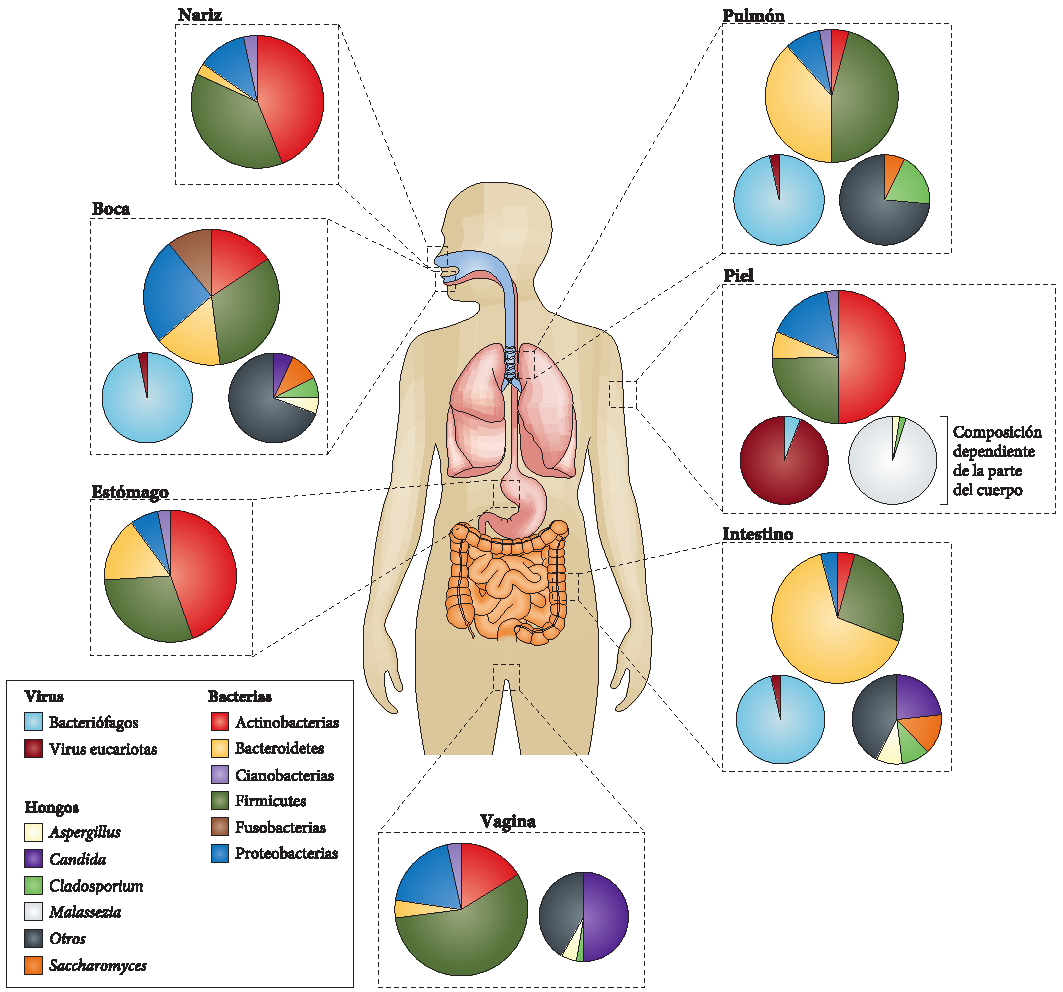
\includegraphics[width=\textwidth]{img/introduction/00_Nichos.pdf}
    \caption[Nichos microbianos]{\textbf{Composición del microbioma en los distintos nichos microbianos.} Esta imagen muestra la distribución y abundancia relativa de las comunidades bacterianas, fúngicas y víricas en distintos lugares del cuerpo humano. La composición bacteriana está representada por los seis filos más abundantes, la composición fúngica por los géneros más destacados y la composición vírica como bacteriófagos o virus eucariotas. Imagen modificada de \cite{marsland2014host}.}
    \label{fig:nichos}
\end{figure}


\subsubsection{Relevancia funcional y clínica del microbioma}

La principal razón para estudiar el microbioma humano es su innegable influencia en la salud y su potencial como diana terapéutica. Este campo de investigación se beneficia de la accesibilidad de muestras no invasivas, como las obtenidas de heces o saliva. Sin embargo, su estudio también se extiende a microambientes más complejos, como el microambiente tumoral, que, aunque requiere métodos más invasivos, es clave para entender el papel de los microorganismos en la progresión del cáncer.

El microbioma es una extensión funcional del genoma humano. Aporta capacidades metabólicas que el ser humano por sí solo no puede codificar, desempeñando un papel clave en la digestión de nutrientes, la síntesis de vitaminas y la desintoxicación de xenobióticos. Por ejemplo, las vías enzimáticas microbianas que metabolizan carbohidratos complejos en ácidos grasos de cadena corta (AGCCs) influyen directamente en el equilibrio energético y las funciones inmunitarias del anfitrión \cite{aggarwal2022microbiome}. Por lo que, al caracterizar la composición y función de la comunidad microbiana, se pueden identificar vías metabólicas e interacciones específicas que influyen en la salud del anfitrión, ofreciendo nuevos objetivos para intervenciones terapéuticas \cite{aggarwal2022microbiome, berg2020microbiome}.

Los cambios y desequilibrios en la composición de estas comunidades, conocidos como disbiosis, se asocian con un amplio rango de enfermedades. Se ha observado que las alteraciones del microbioma pueden preceder a estados patológicos o afectar la respuesta a terapias, lo que posiciona al microbioma como un marcador pronóstico y un objetivo de intervención \cite{das2019homeostasis}.

Además, el microbioma ofrece una gran cantidad de biomarcadores potenciales. Dado que los cambios en la diversidad y abundancia microbiana son indicativos de estados de enfermedad, la identificación de estos patrones tiene un gran potencial para el diagnóstico y el pronóstico \cite{lloyd2016healthy}.

El microbioma humano es muy dinámico e individualizado. Es decir, la variabilidad entre sujetos supera a menudo la observada entre las distintas zonas corporales de un mismo individuo. Esto pone de relieve la complejidad y la naturaleza personalizada de los ecosistemas microbianos. Esta propiedad complica la búsqueda de un microbioma universal «sano», pero también abre vías para enfoques de medicina personalizada en los que los perfiles microbianos pueden guiar estrategias terapéuticas a medida \cite{turnbaugh2007human}.

Finalmente, el microbioma es particularmente adaptable. Las intervenciones dietéticas, las formulaciones probióticas y el trasplante fecal ejemplifican la capacidad de modular estos ecosistemas microbianos, generando resultados beneficiosos sin dañar las células del anfitrión. El hecho de que factores ambientales, dietéticos, el uso de antibióticos y el estilo de vida alteren significativamente la composición del microbioma significa que este puede ser modificado mediante enfoques dirigidos \cite{zmora2019you}.

%% Párrafo conector a secuenciación %%

Comprender la homeostasis microbiana del individuo es esencial. Por ello, la caracterización precisa del microbioma es fundamental, y las técnicas avanzadas de secuenciación son herramientas esenciales para desentrañar la composición microbiana y sentar las bases para la identificación de patrones asociados a estados fisiológicos o patológicos.

%% SECUENCIACIÓN DEL MICROBIOMA %%
\subsection{Caracterización del microbioma}

Históricamente, las investigaciones sobre comunidades microbianas se basaban casi exclusivamente en métodos de cultivo. Los primeros microbiólogos aislaban bacterias cultivándolas en medios selectivos bajo condiciones controladas de laboratorio. Estos métodos de cultivo proporcionaron un punto de entrada tangible para entender los taxones microbianos (por ejemplo, con estudios pioneros como el aislamiento de \textit{Escherichia coli} hace más de un siglo). Sin embargo, estas técnicas tenían limitaciones significativas: eran lentas, laboriosas y sesgadas hacia los organismos que crecían fácilmente \textit{in vitro}. Esto dejaba sin caracterizar una gran parte de la diversidad microbiana, un problema conocido como la «gran anomalía del conteo en placa», donde la cantidad de microorganismos observados al microscopio era mucho mayor que la que se podía cultivar \cite{staley1985measurement, ha2020new}.

La llegada de la secuenciación de nueva generación (NGS, por sus siglas en inglés) representó un cambio de paradigma en la investigación del microbioma al superar muchas de las limitaciones inherentes a las técnicas dependientes del cultivo. Las tecnologías NGS permitieron el perfilado independiente del cultivo y de alto rendimiento de comunidades microbianas complejas directamente a partir de muestras ambientales o clínicas. Plataformas como Roche 454 \cite{454}, Illumina MiSeq/HiSeq \cite{Illumina}, Ion Torrent \cite{Ion} y, posteriormente, enfoques basados en nanoporos y moléculas individuales (por ejemplo, Oxford Nanopore \cite{ON} y Pacific Biosciences \cite{PacBio}) proporcionaron a los investigadores una profundidad, velocidad y resolución sin precedentes en la secuenciación de genomas microbianos \cite{goodwin2016coming}.

Gracias a la alta resolución de estas plataformas de NGS, es posible no solo identificar los microorganismos presentes, sino también clasificarlos en distintos niveles taxonómicos (Figura \ref{fig:niveles}). Estos niveles abarcan desde dominios y filos hasta géneros y especies, lo que facilita una caracterización exhaustiva de la estructura y diversidad de las comunidades microbianas. Esta alta resolución facilita la detección de patrones microbianos sutiles y la identificación de taxones que pueden servir como biomarcadores clínicos, aportando información valiosa para el diagnóstico y el desarrollo de terapias personalizadas \cite{hugerth2017analysing}.

\begin{figure}[h]
    \centering
    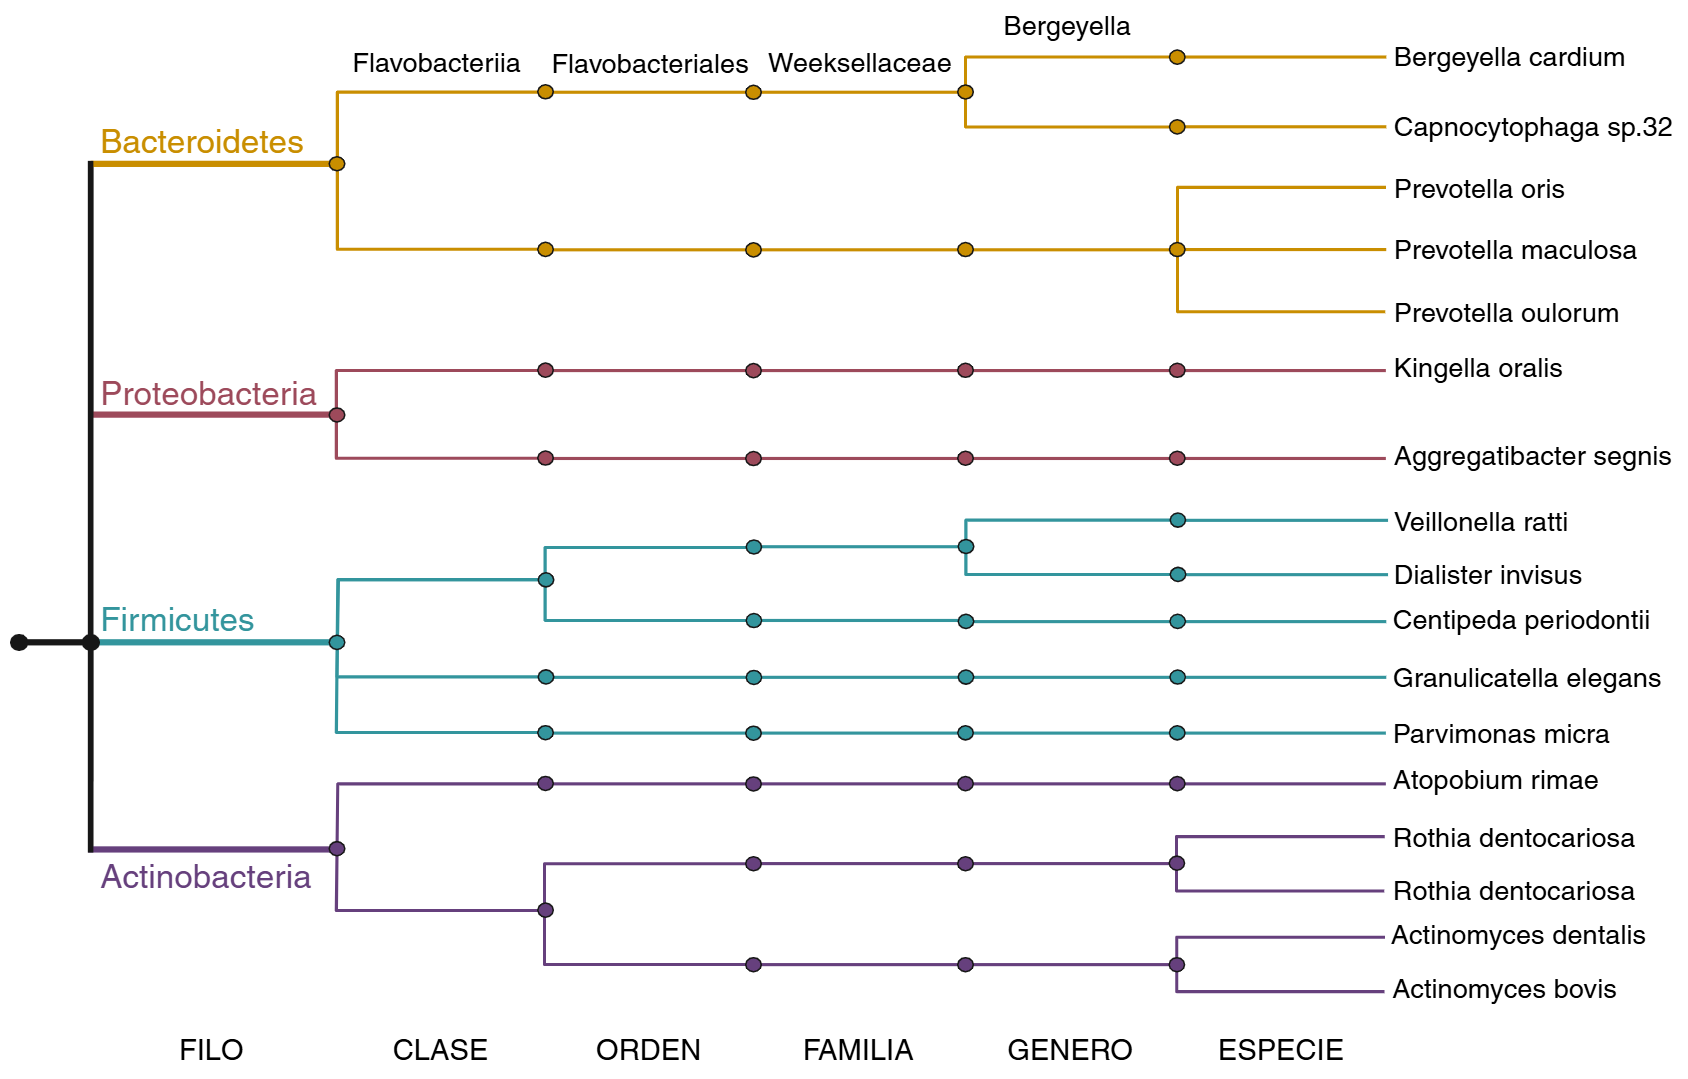
\includegraphics[width=\textwidth]{img/introduction/01_Niveles.png}
    \caption[Niveles taxonómicos]{\textbf{Ejemplo de niveles taxonómicos en el dominio bacteriano}. La imagen representa la división taxonómica de 4 filos bacterianos. Este árbol es una representación de clasificación filogenética a diferentes niveles de resolución, desde filo hasta especie. Imagen creada con BioRender \cite{biorender2025}.}
    \label{fig:niveles}
\end{figure}

En esta Tesis Doctoral, el enfoque seleccionado para la caracterización del microbioma se centra en analizar su composición a través de la metagenómica, uno de los métodos más utilizados para estudiar el microbioma. Este enfoque puede emplear dos estrategias: la secuenciación del gen que codifica el ARN ribosómico bacteriano 16S (16S rRNA, por sus siglas en inglés) y la secuenciación del genoma completo (WGS, por sus siglas en inglés) \cite{bharti2021current}.

\subsubsection{Secuenciación del gen 16S rRNA}

La secuenciación del gen 16S rRNA es una de las estrategias más utilizadas en la caracterización del microbioma. Este gen, de aproximadamente 1.500 pares de bases, contiene regiones muy conservadas (C1-C10) que permiten el diseño de \textit{primers} universales para la reacción en cadena de la polimerasa (PCR, por sus siglas en inglés). Además, estas regiones conservadas flanquean nueve regiones hipervariables (V1-V9), cuyas secuencias son únicas para diferentes taxones. Esta combinación de regiones, plasmada en la Figura \ref{fig:RNAr_16S}, permite una identificación taxonómica precisa de una amplia variedad de bacterias y arqueas presentes en una determinada comunidad microbiana \cite{knight2018best}.

\begin{figure}
    \centering
    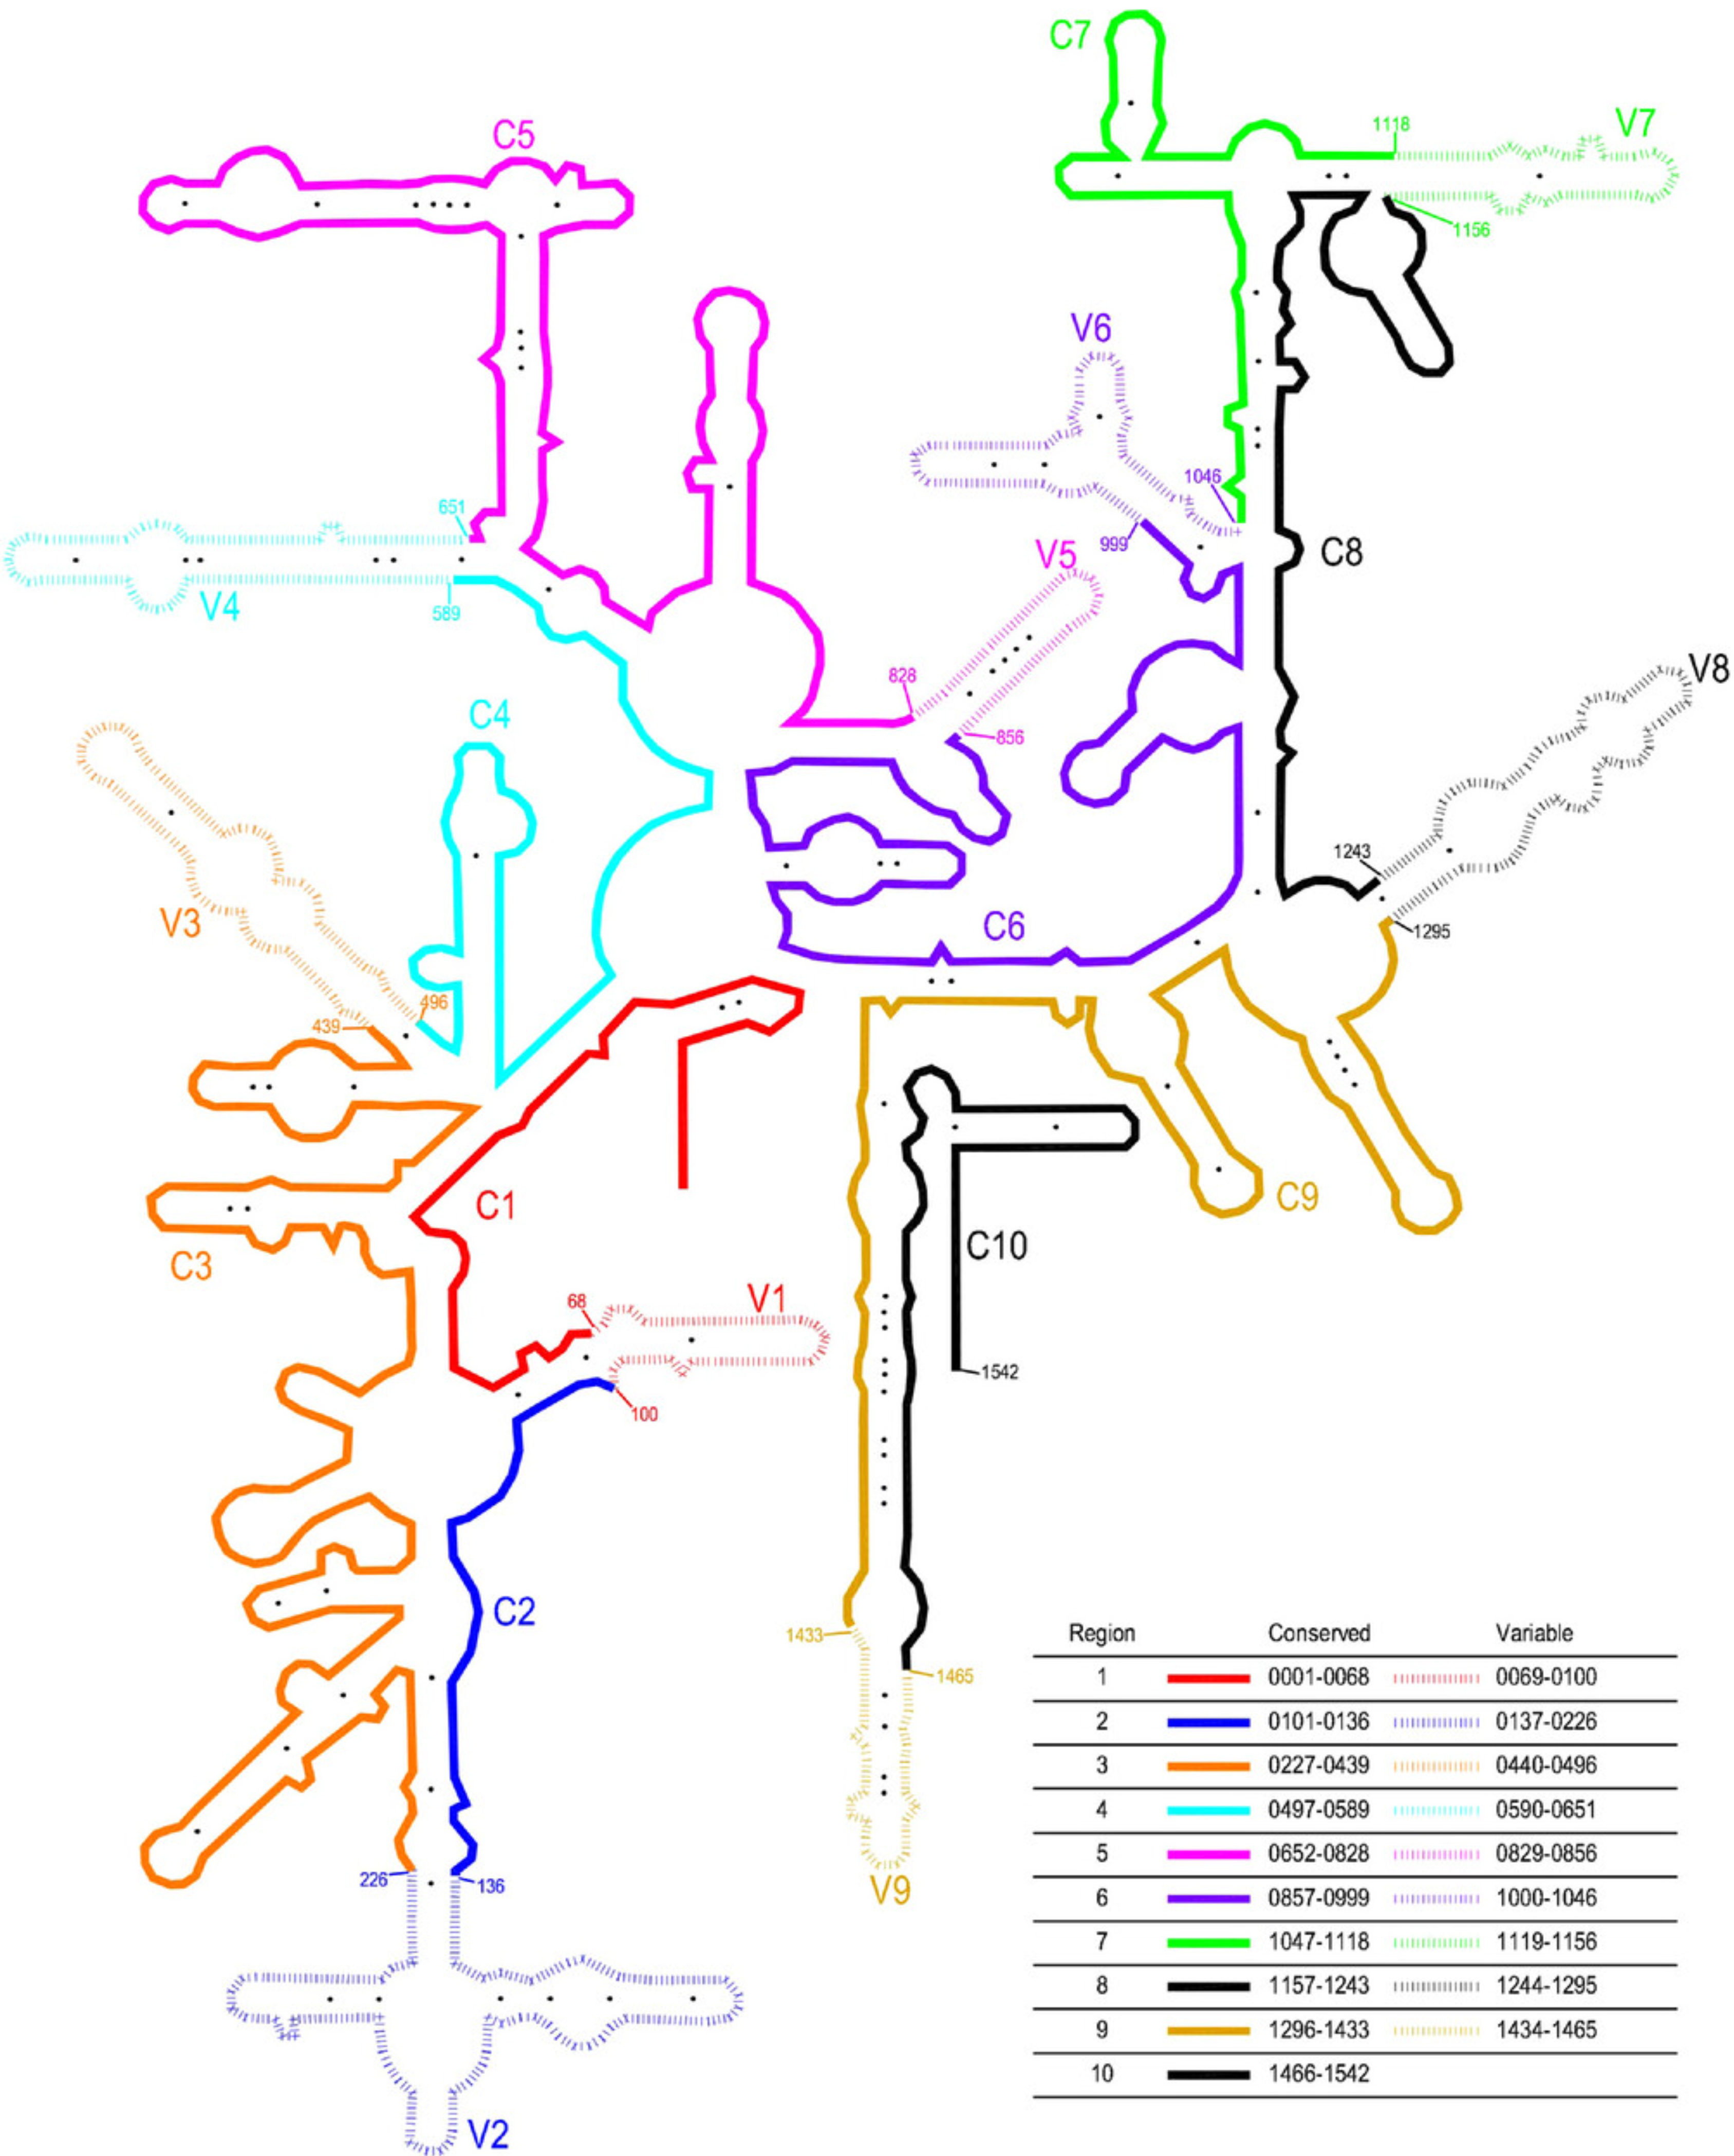
\includegraphics[width=\textwidth]{img/introduction/02_16S.jpeg}
    \caption[Estructura secundaria del gen 16S rRNA.]{\textbf{Estructura secundaria del gen 16S rRNA.} La imagen ilustra la estructura secundaria coloreada por las regiones que conforman el gen, indicado las zonas conservadas (C) y las zonas variables (V). Imagen modificada de \cite{regueira2023critical}.}
    \label{fig:RNAr_16S}
\end{figure}

Gracias a estas características, la secuenciación 16S rRNA sigue siendo la técnica más utilizada en la taxonomía microbiana y proporciona un acceso sencillo para evaluar la composición de comunidades microbianas en muestras clínicas. La elección de distintos conjuntos de \textit{primers} que se dirigen a regiones variables específicas, como V1-V2, V3-V4 o V4, puede afectar la sensibilidad y resolución del análisis, así como introducir posibles sesgos.\cite{regueira2023critical, yang2016sensitivity}.


\textbf{Procesamiento bioinformático: de las OTUs a las ASVs}

Después de la secuenciación, el procesamiento bioinformático es crucial para interpretar los datos. Tradicionalmente, las secuencias obtenidas en este tipo de secuenciación se agrupaban en Unidades Taxonómicas Operacionales (OTUs, por sus siglas en inglés) basadas en un umbral de similitud predefinido. Aunque este enfoque basado en OTUs mitigaba el impacto de los errores de secuenciación al agrupar secuencias similares, enfrentaba varios inconvenientes. La naturaleza arbitraria de los umbrales de similitud puede resultar en la fusión de taxones distintos en una sola OTU (ver Figura \ref{fig:OTUS}), lo que puede oscurecer variaciones biológicas a pequeña escala y llevar a resultados inconsistentes al comparar conjuntos de datos generados con diferentes umbrales o métodos. En muchos casos, el uso de OTUs puede subestimar la verdadera diversidad microbiana y distorsionar métricas ecológicas como la riqueza de especies, dominancia y equidad \cite{edgar2018updating}.

En respuesta a estos desafíos, ha surgido un cambio metodológico con el desarrollo de algoritmos de eliminación de ruido e inferencia biológica diseñados para resolver Variantes de Secuencias de Amplicones (ASVs, por sus siglas en inglés) \cite{callahan2016dada2}. A diferencia de las OTUs, las ASVs no dependen de umbrales de similitud arbitrarios; en su lugar, buscan distinguir las secuencias biológicas verdaderas de los errores de secuenciación aplicando modelos estadísticos de error a los datos observados. Este enfoque proporciona resolución a nivel de un solo nucleótido, permitiendo la identificación de variantes microbianas con mayor precisión y reproducibilidad entre estudios (ver Figura \ref{fig:OTUS}).

La mayor resolución de los métodos basados en ASV es particularmente ventajosa para el descubrimiento de biomarcadores, ya que diferencias sutiles en la estructura de la comunidad microbiana y la presencia de taxones de baja abundancia pueden tener implicaciones biológicas y clínicas significativas. Además, la naturaleza estandarizada de las ASVs facilita las comparaciones entre estudios \cite{callahan2017exact}.

\begin{figure}
    \centering
    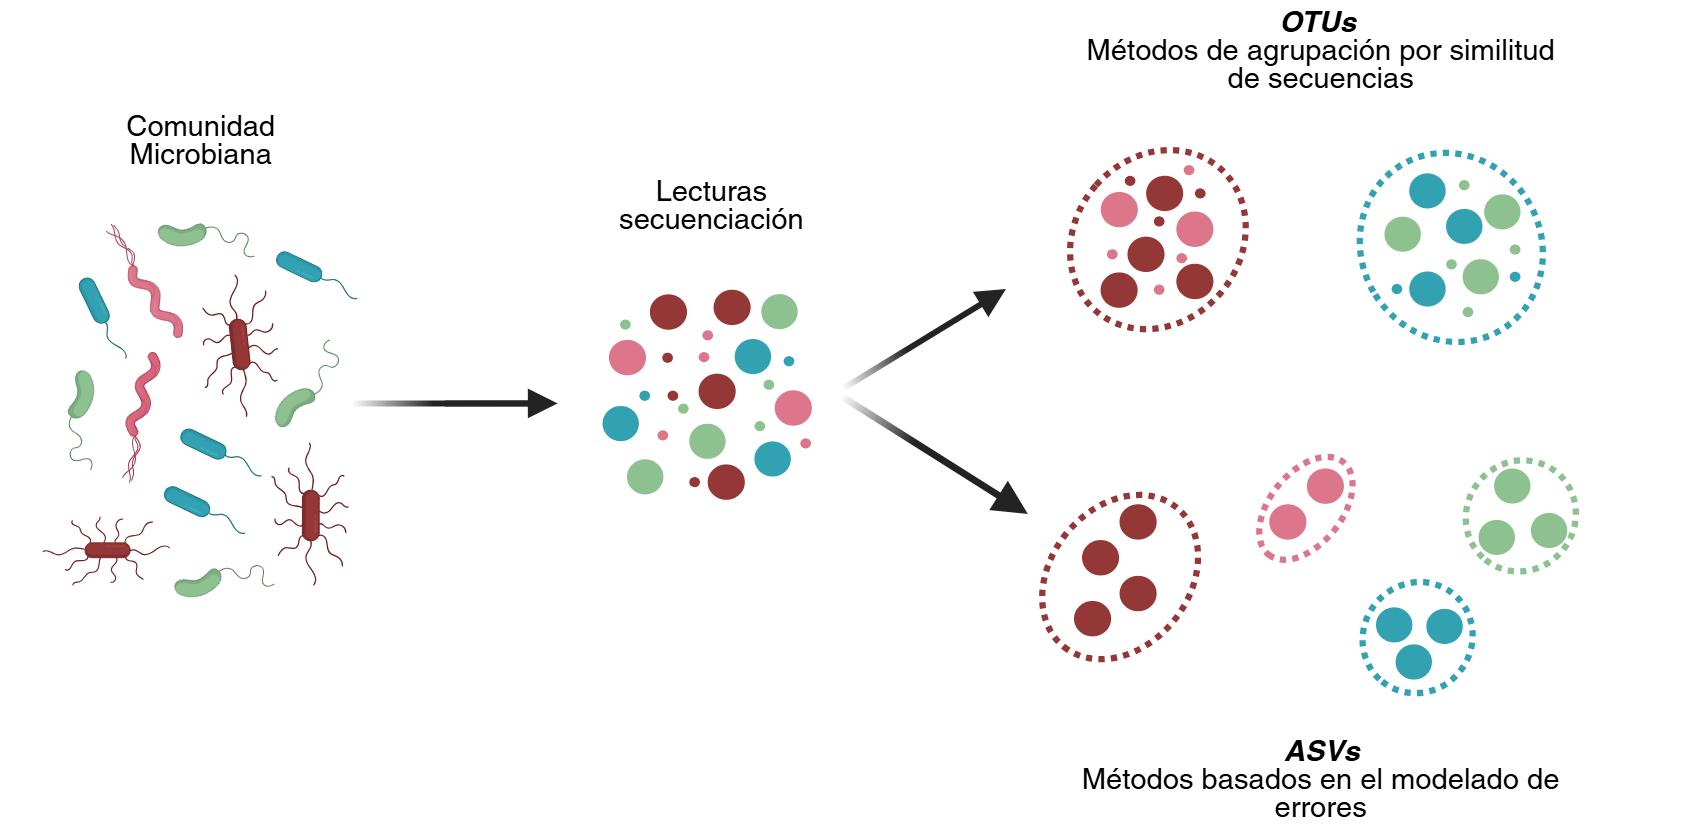
\includegraphics[width=\textwidth]{img/introduction/03_OTUs_ASVs.png}
    \caption[Comparación OTUs y ASVs]{\textbf{Comparación esquemática entre OTUs y ASVs.} Esta imagen ilustra cómo la agrupación de secuencias en OTUs considera similitudes generales, mientras que las ASVs reflejan diferencias específicas a nivel de secuencia individual y eliminando posibles secuencias quiméricas. Imagen creada con BioRender \cite{biorender2025}.}
    \label{fig:OTUS}
\end{figure}

\subsubsection{Secuenciación del genoma completo}

La secuenciación WGS surge como un enfoque complementario a la secuenciación 16S rRNA, superando ciertas limitaciones de esta última, como los sesgos de \textit{primers} y la resolución limitada. WGS involucra la fragmentación aleatoria del ADN total de una muestra, permitiendo la secuenciación de ADN bacteriano, viral, fúngico y arqueal. Además, este enfoque no se limita a la amplificación de un solo gen, lo que facilita un perfil taxonómico más detallado y una caracterización funcional más completa de las comunidades microbianas, permitiendo la identificación de genes y rutas metabólicas (ver Figura \ref{fig:sequencing}).

En este tipo de secuenciación, el enfoque estándar es el basado en referencias, es decir, las lecturas de secuenciación se procesan mediante algoritmos de mapeo que alinean cada lectura a colecciones de genes y genomas previamente caracterizados en bases de datos curadas. Este enfoque utiliza herramientas de clasificación taxonómica que se valen de estrategias de homología y perfiles de secuencias para asignar una etiqueta taxonómica y funcional a cada lectura o fragmento mapeado \cite{bharti2021current}.

Al comparar la secuenciación del gen 16S rRNA con WGS, cada enfoque presenta fortalezas y debilidades distintas. Mientras que el 16S rRNA es una opción rentable para el perfilado comunitario a gran escala, la WGS proporciona una visión holística y funcional de la comunidad microbiana. La complejidad, el costo y los requisitos computacionales de la WGS la hacen menos accesible para estudios de rutina, pero son invaluables para la caracterización profunda del microbioma.

%% Justificación 16S Tesis Doctoral %%

Esta Tesis Doctoral se ha basado en el análisis de datos de secuenciación del gen 16S rRNA, considerando que este enfoque ofrece un equilibrio adecuado entre accesibilidad, reproducibilidad y capacidad de caracterización microbiana para los objetivos planteados. La secuenciación 16S rRNA permite obtener perfiles taxonómicos consistentes y comparables entre diferentes estudios y cohortes, lo que resulta especialmente útil para la identificación de patrones microbianos potencialmente asociados a procesos patológicos. Su menor demanda computacional y su amplia disponibilidad de datos públicos facilitan la realización de análisis extensivos y la validación externa de resultados, aspectos clave en la búsqueda de biomarcadores robustos. Además, la estandarización de las metodologías asociadas al 16S rRNA contribuye a la reproducibilidad y fiabilidad de los hallazgos, elementos fundamentales en investigaciones orientadas a la traslación clínica. En conjunto, estas características hacen del enfoque 16S rRNA una herramienta adecuada para explorar y detectar señales microbianas relevantes en el contexto del diagnóstico de enfermedades.

\begin{figure}
    \centering
    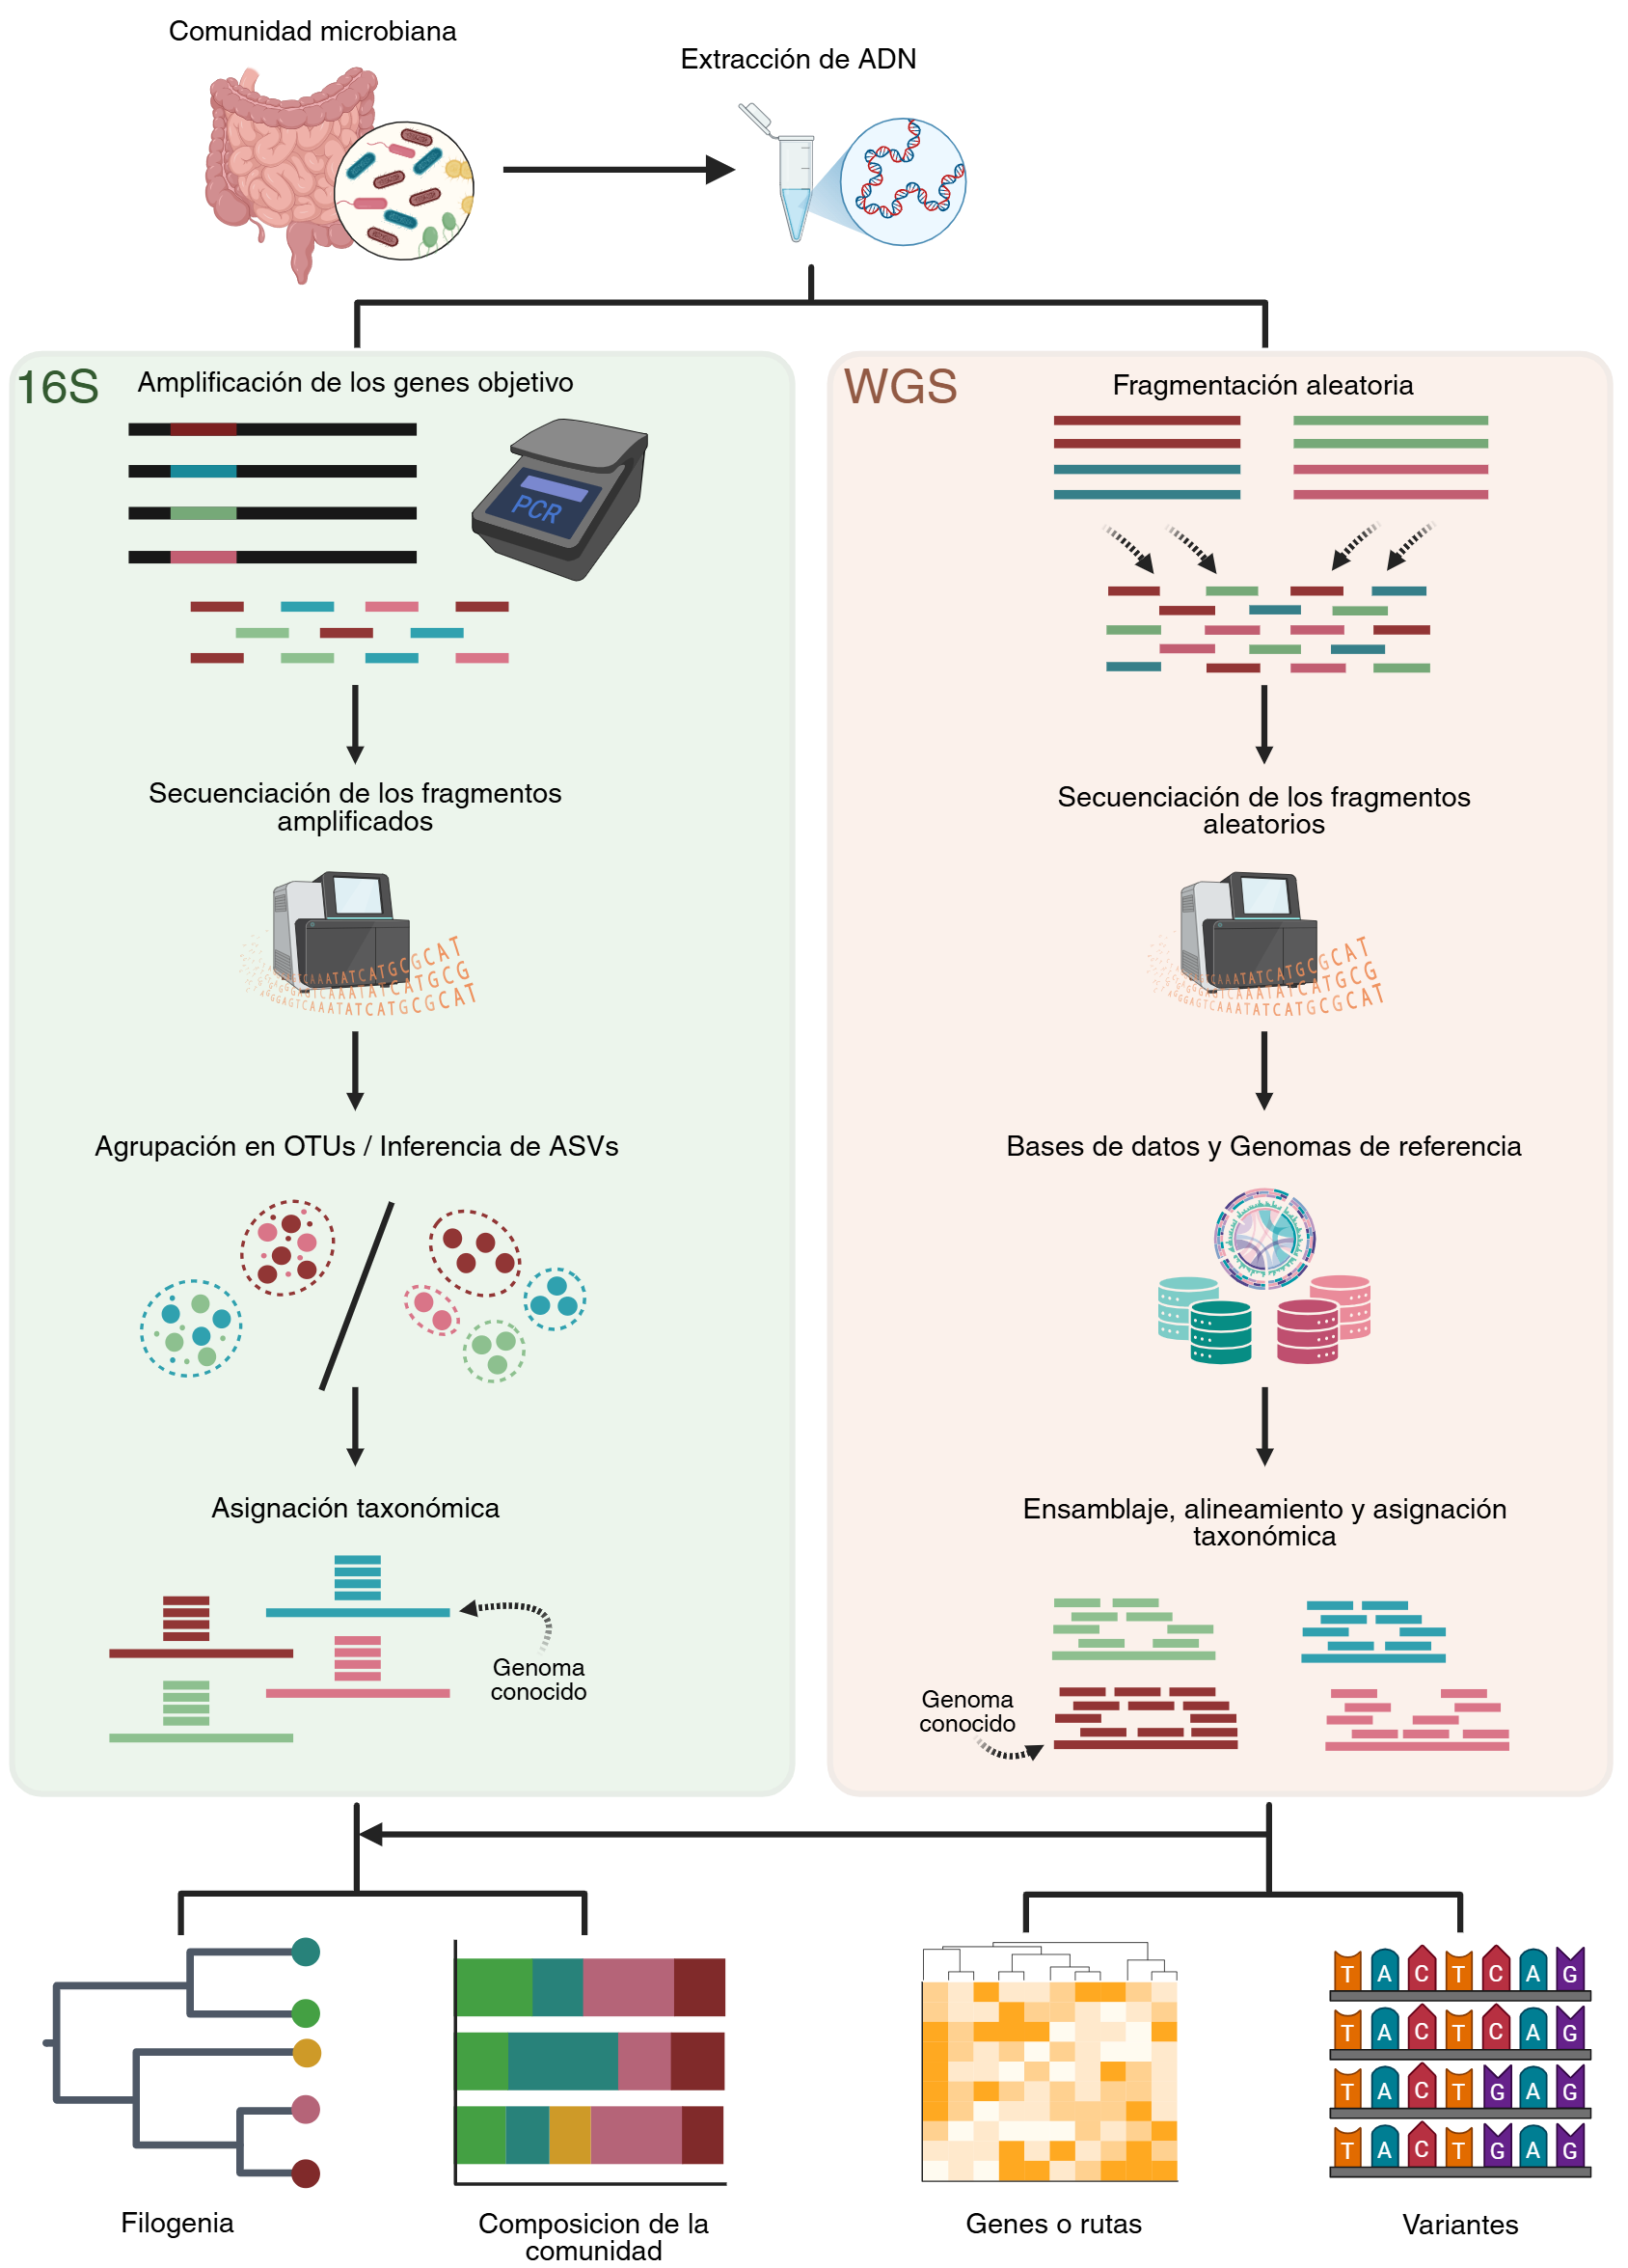
\includegraphics[width=\textwidth]{img/introduction/04_Secuenciacion.png}
    \caption[Comparación 16S rRNA y WGS]{\textbf{Diagrama comparativo del análisis de comunidades microbianas mediante 16S rRNA y WGS.} El flujo de trabajo ilustra cómo la sencuenciación 16S rRNA utiliza la amplificación de genes objetivo para identificar OTUs o ASVs y asignar taxonomía. Mientras que, WGS, utiliza fragmentación aleatoria para secuenciar todo el genoma, seguido de ensamblaje y alineamiento, con la finalidad de analizar filogenia, composición comunitaria, genes, rutas y variantes. Imagen creada con BioRender \cite{biorender2025}.}
    \label{fig:sequencing}
\end{figure}

%% Párrafo conector a secuenciación %%

La caracterización del microbioma mediante métodos de secuenciación ha promovido la investigación a gran escala, llevando a la financiación de grandes proyectos internacionales y la creación de bases de datos públicas. Estas iniciativas han resaltado la importancia de este campo, proporcionando recursos valiosos para la investigación. Estas plataformas facilitan el avance del conocimiento y permiten la colaboración global en la búsqueda de nuevos biomarcadores y en la comprensión de las comunidades microbianas.

%%  3. Recursos para Microbioma  %%
\subsection{Recursos de datos públicos para el análisis del microbioma humano}

El auge en la generación de datos del microbioma proviene de mejoras revolucionarias en las plataformas de secuenciación que, al reducir costos e incrementar la capacidad, han permitido a los investigadores secuenciar miles de muestras con gran profundidad y resolución. Como ya se ha comentado, los estudios iniciales estaban limitados por métodos basados en cultivos y técnicas de baja capacidad que ofrecían una visión parcial del mundo microbiano; sin embargo, la llegada de métodos independientes del cultivo, como la secuenciación 16S rRNA y WGS, ha revelado la inmensa complejidad y riqueza funcional de las comunidades microbianas.

\subsubsection{Proyecto Microbioma Humano}

El Proyecto del Microbioma Humano (HMP, por sus siglas en inglés), impulsado por los \textit{National Institutes of Health} en 2007, es uno de los esfuerzos más ambiciosos para generar un catálogo de referencia integral del microbioma humano. Su objetivo principal era caracterizar las comunidades microbianas en múltiples sitios anatómicos, estandarizando protocolos de muestreo, desarrollando técnicas experimentales y generando conjuntos de datos. El HMP fue concebido en respuesta al creciente reconocimiento de que una comprensión profunda del microbioma humano era crucial para esclarecer sus roles en estados fisiológicos y patológicos \cite{turnbaugh2007human}.

En su primera fase, representada como HMP1 en la Figura \ref{fig:HMP}, se muestrearon aproximadamente 300 adultos sanos en cinco hábitats corporales principales: cavidad oral, piel, fosas nasales, tracto gastrointestinal y tracto urogenital, resultando en la recolección de más de 11.000 muestras físicas. De estas, casi 10.000 fueron analizadas por secuenciación de 16S rRNA, mientras que un subconjunto estratégico de aproximadamente 2.300 muestras se sometió a secuenciación WGS. Esta fase produjo recursos esenciales como catálogos de genomas de referencia, protocolos clínicos estandarizados y herramientas computacionales para el análisis de datos procedentes de 16S rRNA y WGS, facilitando futuras investigaciones enfocadas en enfermedades \cite{aagaard2013human}.

La segunda fase, representada como HMP2 en la Figura \ref{fig:HMP}, amplió el alcance centrándose en el estudio de enfermedades (parto prematuro, enfermedad inflamatoria intestinal y diabetes) y utilizando enfoques multiómicos para integrar la composición microbiana con datos biológicos del anfitrión \cite{integrative2014integrative}.


\begin{figure}
    \centering
    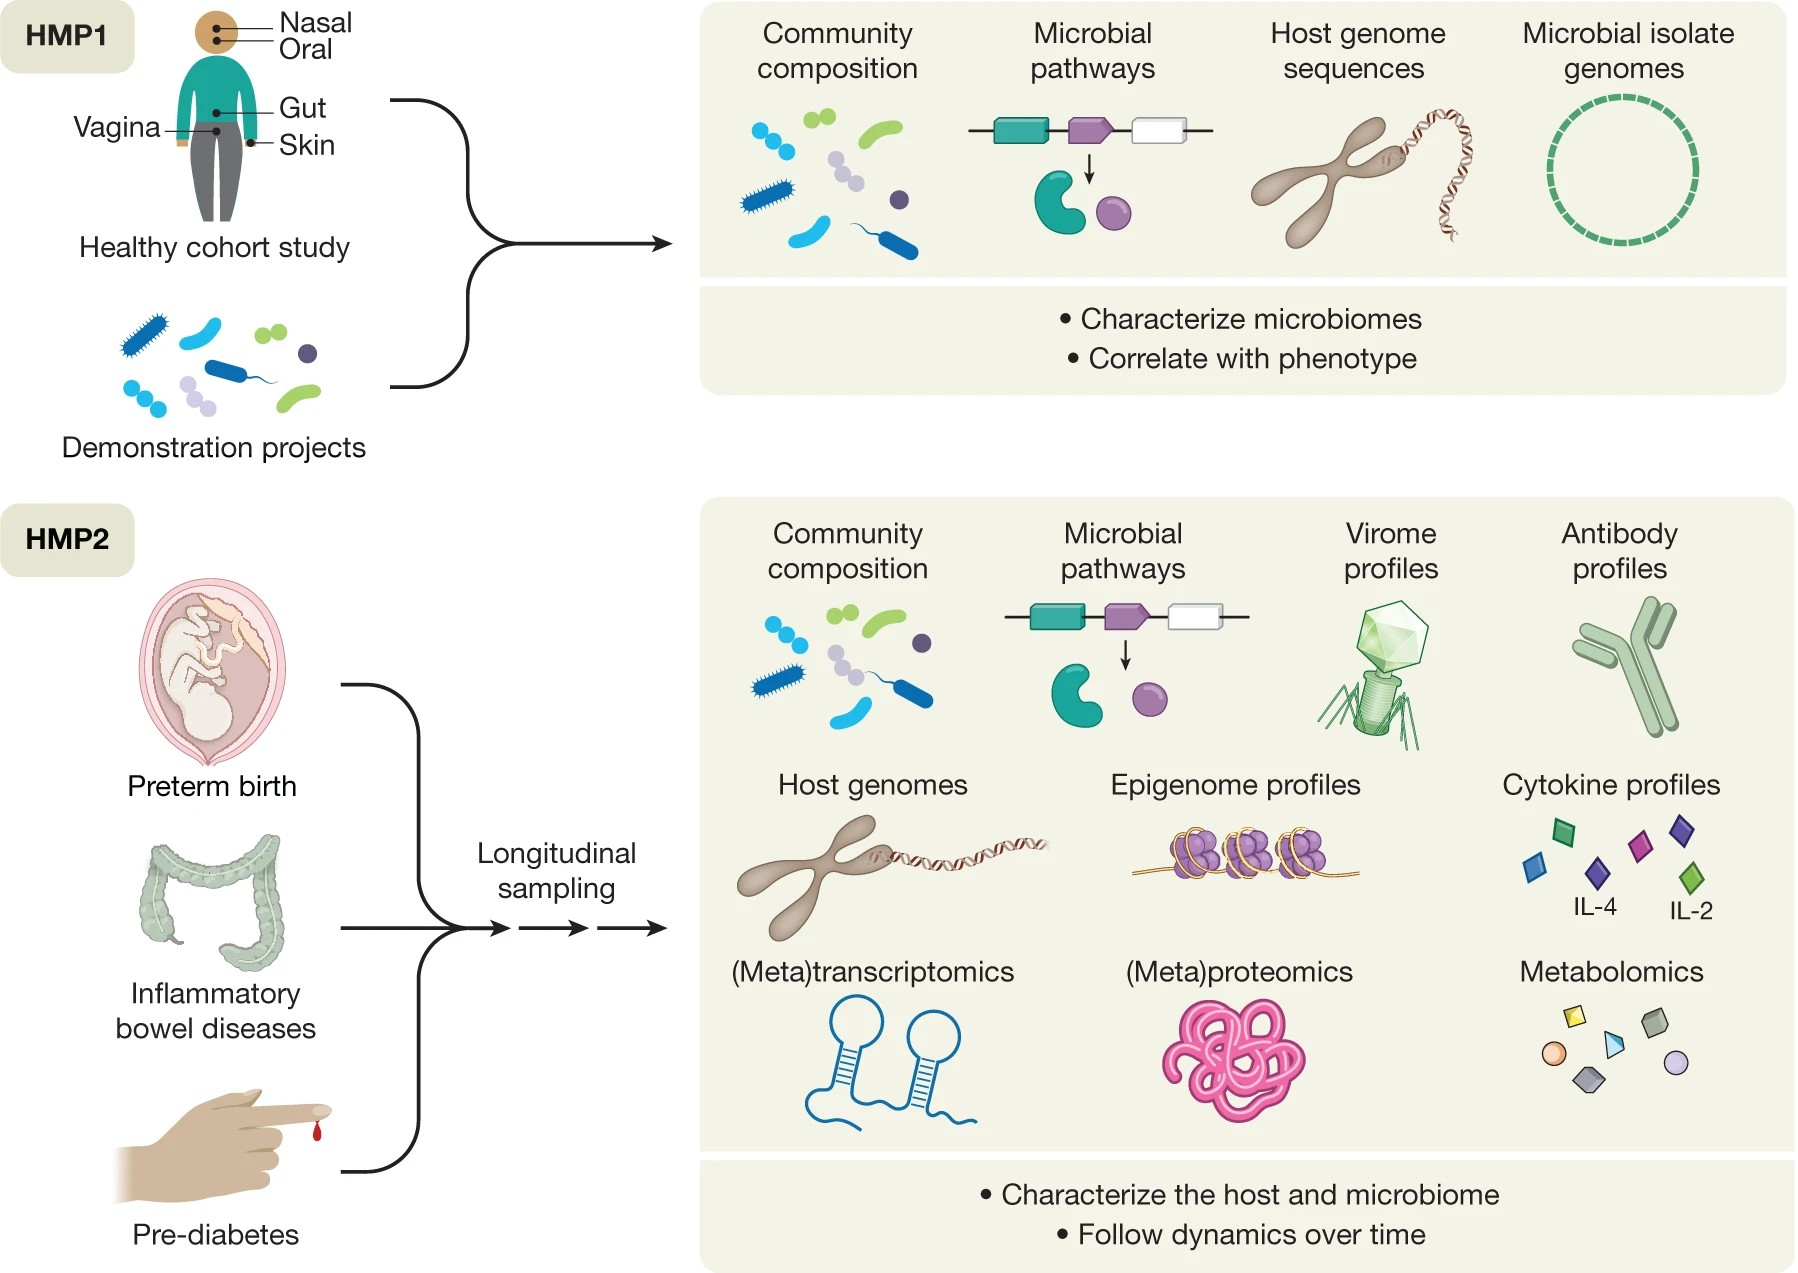
\includegraphics[width=0.99\textwidth]{img/introduction/HMP.jpg}
    \caption[Fases del HMP]{\textbf{Ilustración de las fases del HMP.} El HMP1 se centró en estudiar el microbioma en cohortes sanas a través de análisis de composición microbiana, genomas microbianos y correlaciones con fenotipos. El HMP2 expandió el enfoque hacia condiciones específicas como partos prematuros y enfermedades inflamatorias intestinales, utilizando muestreos longitudinales y diferentes perfiles ómicos. Imagen extraída de \cite{integrative2014integrative}.}
    \label{fig:HMP}
\end{figure}


\subsubsection{Proyecto DIABIMMUNE}

Surgiendo en paralelo con iniciativas más amplias como el HMP, el proyecto DIABIMMUNE representa un esfuerzo enfocado en dilucidar el papel de la higiene y del microbioma en patologías autoinmunes, particularmente la diabetes tipo 1 (DT1). Fue motivado por la necesidad de identificar factores microbianos que no solo se correlacionen, sino que potencialmente impulsen el inicio y la progresión de condiciones autoinmunes. Este proyecto utiliza muestreo longitudinal de poblaciones en riesgo, aplicando NGS y enfoques multiómicos integrativos para rastrear la sucesión microbiana y correlacionar cambios en la microbiota intestinal con marcadores inmunológicos y resultados clínicos \cite{DIABIMMUNE_project}.

Mientras que el HMP se diseñó para obtener datos de referencia de individuos sanos, el proyecto DIABIMMUNE tiene un objetivo centrado en la enfermedad: identificar biomarcadores microbianos que predigan el riesgo y explicar la conexión entre el desequilibrio microbiano y la autoinmunidad. Al analizar comparativamente muestras de individuos predispuestos a la DT1 y contrastarlas con controles sanos, el proyecto ha producido valiosos conjuntos de datos que no solo validan observaciones previas que vinculan el microbioma intestinal con la modulación inmune, sino que también abren camino a intervenciones terapéuticas guiadas por el microbioma \cite{kostic2015dynamics, mustonen2018early, miettinen2022breastfeeding}.

Los datos utilizados para la realización del segundo trabajo \cite{paper2} que conforma esta Tesis Doctoral fueron extraídos de este proyecto.


\subsubsection{Proyecto IBEROBDIA}

El proyecto «Obesidad y diabetes en Iberoamérica: Factores de riesgo y nuevos biomarcadores patogénicos y predictivos» (IBEROBDIA) es un proyecto iberoamericano formado por ocho grupos de investigación de cinco países diferentes (Argentina, Chile, Colombia, España y México). Este proyecto tiene como objetivos: identificar factores de riesgo para el desarrollo de la obesidad y de diabetes tipo 2 (DT2) y la identificación de nuevos biomarcadores biológicos para la predicción y diagnóstico de DT2 \cite{IBEROBDIA_project}. Para ello, se realizó un cribado y se incluyó a pacientes con riesgo de sufrir DT2, de entre 40 y 70 años. A estos pacientes se les realizaron diferentes pruebas clínicas para caracterizarlos en distintos grupos de estudio. Finalmente, se les extrajeron muestras fecales a las que se les realizó la secuenciación 16S rRNA.

En el marco de la contribución al nodo español de IBEROBDIA, se llevó a cabo el reclutamiento y análisis de 79 muestras procedentes de pacientes diagnosticados con un amplio espectro de patologías, con el fin de generar el conjunto de datos de referencia; dicho conjunto de datos fue analizado en el primer trabajo \cite{paper1} que conforma esta Tesis Doctoral.

\subsubsection{Archivo Europeo de Nucleótidos}

A medida que la generación de datos supera rápidamente los métodos tradicionales de gestión, la necesidad de soluciones de almacenamiento robustas e interoperables se ha vuelto crucial. El enorme volumen de datos generado por grandes consorcios como el HMP, proyectos transnacionales como DIABIMMUNE o IBEROBDIA, así como por estudios a menor escala realizados por investigadores individuales, ha llevado al desarrollo de varios repositorios clave que sirven como pilares para la comunidad de investigación del microbioma.

Entre estos repositorios, el Archivo Europeo de Nucleótidos (ENA, por sus siglas en inglés) desempeña un papel crítico. Este es esencial para el almacenamiento a largo plazo y la difusión de datos de secuenciación en bruto, incluyendo no solo datos de microbioma, sino también de genómica y transcriptómica, entre otros. Diseñado para archivar grandes cantidades de datos generados por plataformas de alta capacidad, el ENA asegura que estos conjuntos de datos estén disponibles para reanálisis y validación por la comunidad científica en general \cite{leinonen2010european}. Al proporcionar acceso robusto a lecturas sin procesar, el ENA sustenta la reproducibilidad de los estudios del microbioma y permite a los investigadores implementar metodologías innovadoras sobre datos reales, facilitando análisis innovadores que podrían ser difíciles de realizar de otra manera.

Gracias a la disponibilidad de datos crudos de 16S rRNA en el ENA se ha podido realizar el tercer trabajo \cite{paper3} de esta Tesis Doctoral. Específicamente, se han descargado muestras de microbioma vaginal de 5 cohortes diferentes: SRA022855 \cite{ravel2011vaginal}, SRA051298 \cite{srinivasan2012bacterial}, PRJNA208535 \cite{ravel2013daily}, PRJNA797778 \cite{france2022insight} y PRJNA302078 \cite{xiao2016predictive} (la información detallada de cada cohorte se puede consultar en la metodología del tercer trabajo \cite{paper3}). Esto ha permitido llevar a cabo un subtipado de perfiles microbianos vaginales en el contexto de la vaginosis bacteriana (VB).


%% Párrafo conector a Dificultades %%

La existencia de estos recursos de datos públicos, como los proporcionados por el HMP, DIABIMMUNE o IBEROBDIA, ha democratizado el acceso a datos e información sobre el microbioma humano. Sin embargo, el análisis de estos datos no está exento de desafíos. A pesar de la abundancia de información, estudiar el microbioma presenta dificultades y limitaciones metodológicas y conceptuales que deben ser consideradas para obtener resultados precisos y clínicamente relevantes.

\subsection{Desafíos del estudio del microbioma}

El análisis del microbioma humano se enfrenta a una serie de desafíos metodológicos y conceptuales que limitan la interpretación de sus resultados. La naturaleza dinámica de estas comunidades microbianas, junto con las particularidades técnicas y analíticas de los datos, introduce múltiples niveles de complejidad. A continuación, se detallan las principales dificultades inherentes a su estudio.

Una de las principales limitaciones es la elevada variabilidad de la composición microbiana, tanto entre distintos individuos (interindividual) como en un mismo sujeto a lo largo del tiempo (intraindividual). Esta heterogeneidad dificulta la definición de un microbioma «central» o universalmente sano y obliga a diseñar estudios con cohortes de gran tamaño para controlar las numerosas variables de confusión. A esta complejidad se suma la dificultad para diferenciar entre microorganismos residentes, que forman parte estable del ecosistema, y colonizadores transitorios, cuya presencia puede introducir sesgos en la interpretación funcional \cite{fu2019temporal, lyu2023methodological}.

Las comunidades microbianas no son colecciones de organismos aislados, sino redes complejas y dinámicas. Las interacciones entre distintos taxones, así como entre los microorganismos y las células del anfitrión, son fundamentales para la función del ecosistema. Un factor que complica adicionalmente su estudio es la redundancia funcional, fenómeno por el cual diferentes especies microbianas pueden desempeñar roles metabólicos similares. Esta característica hace que la tarea de asociar un taxón específico con un resultado clínico concreto sea particularmente compleja \cite{zuniga2017elucidation, layeghifard2017disentangling}.

Finalmente, el tratamiento de los datos generados mediante NGS presenta desafíos estadísticos y bioinformáticos sustanciales. Estos datos son inherentemente composicionales, dispersos y presentan una alta proporción de ceros. Estas características estructurales limitan la aplicabilidad de los métodos estadísticos convencionales, que pueden no capturar adecuadamente las relaciones subyacentes. Por tanto, se requiere el uso de herramientas bioinformáticas y modelos estadísticos especializados para su correcto análisis \cite{gloor2016compositional, pan2021statistical}.


%% Párrafo conector a Eubiosis y Disbiosis %%

A pesar de estas dificultades para definir una composición microbiana universalmente «sana», la investigación se ha centrado en el concepto de equilibrio funcional del ecosistema. Este estado de homeostasis, denominado eubiosis, se considera un pilar para la salud del anfitrión. Por el contrario, la pérdida de este equilibrio, conocida como disbiosis, se ha asociado con el desarrollo o la progresión de diversas patologías. La transición entre estos dos estados es, por tanto, un marco conceptual clave para comprender la influencia del microbioma en la patogénesis de diferentes enfermedades.


\subsection{Equilibrio microbiano}

Hasta hace unas décadas, el rol y la importancia que tiene el microbioma en la homeostasis del individuo eran poco conocidos, por lo que también se desconocía su implicación en el origen o progresión de cualquier enfermedad. Gracias a iniciativas a gran escala, como el HMP, se ha podido caracterizar las comunidades microbianas de distintos nichos corporales, revelando su profunda implicación en la salud. Se ha demostrado que las relaciones mutualistas entre estos microorganismos y las células humanas a nivel endocrino, neurológico e inmunológico son de vital importancia para el correcto funcionamiento del organismo.

El equilibrio de estas interacciones se conoce como eubiosis. Este estado se caracteriza, en la mayoría de los nichos, por una alta diversidad microbiana donde se establecen interacciones beneficiosas entre los microorganismos y el anfitrión. Una comunidad microbiana eubiótica contribuye a mantener un entorno antiinflamatorio, lo que impacta positivamente en la salud. En contraste, la alteración de este equilibrio se denomina disbiosis. Este estado se asocia a una reducción de la biodiversidad microbiana y favorece la proliferación de patógenos oportunistas. En consecuencia, una condición disbiótica puede promover un estado proinflamatorio sistémico y contribuir al desarrollo de diversas enfermedades \cite{petersen2014defining, gao2015microbiota}.

En el marco de esta Tesis Doctoral se analizan dos ecosistemas microbianos de particular relevancia clínica: el intestinal y el vaginal. Ambos presentan características distintivas y cumplen funciones esenciales. El microbioma intestinal, con su elevada diversidad, influye de manera crítica en la digestión y la modulación del sistema inmunitario. Por su parte, el microbioma vaginal, habitualmente dominado por un solo género, desempeña un papel crucial en la defensa contra infecciones y en el mantenimiento de la salud reproductiva.

\subsubsection{El Microbioma Intestinal}

%% El Microbioma Intestinal %%
%%% Microbioma intestinal sano %%%

Como se puede observar en la Figura \ref{fig:gut}, un microbioma intestinal en estado de eubiosis se caracteriza principalmente por una elevada diversidad microbiana. La composición de un microbioma intestinal sano a nivel de filo se caracteriza por una abundancia predominante de Firmicutes y Bacteroidetes (90\%) en comparación con Actinobacteria (5-10\%) y Proteobacteria (1-5\%), entre otras \cite{rinninella2019healthy}. Las bacterias beneficiosas, especialmente los Firmicutes y Bacteroidetes, desempeñan un papel crucial en la digestión de alimentos, particularmente de carbohidratos no digeribles como la fibra. Mediante la fermentación de esta fibra, producen metabolitos beneficiosos como los AGCCs, que son fundamentales para la salud intestinal. Estos AGCCs (incluyendo el acetato, propionato y butirato) proporcionan energía a las células del colon, ayudan a mantener la integridad de la mucosa intestinal y poseen propiedades antiinflamatorias. Además de proporcionar energía, los AGCCs también contribuyen a la regulación del metabolismo lipídico y glucídico, promoviendo un estado de homeostasis en el cuerpo \cite{rinninella2019healthy, flint2012role}. A mayores, la mucosa intestinal, que actúa como una barrera entre el contenido intestinal y el torrente sanguíneo, se ve favorecida por la presencia de un microbioma diverso. La producción de mucinas por las bacterias beneficiosas contribuye a la formación de una capa protectora que ayuda a prevenir la translocación de patógenos y toxinas hacia el sistema circulatorio. Además, estas bacterias beneficiosas segregan péptidos antimicrobianos que inhiben el crecimiento de microorganismos patógenos \cite{cani2016talking, alvarez2021gut}.

%%% Microbioma intestinal desequilibrado %%%

Sin embargo, en un estado de disbiosis intestinal (Figura \ref{fig:gut}), la reducción de microorganismos capaces de producir metabolitos beneficiosos lleva a una disminución de la energía disponible para las células epiteliales del colon, afectando la integridad de la mucosa intestinal y aumentando la vulnerabilidad a la inflamación y la invasión de patógenos. La proliferación de estos microorganismos patógenos, como \textit{Escherichia coli} o \textit{Clostridium difficile}, puede desplazar a las especies beneficiosas, comprometiendo aún más la homeostasis del microbioma. Además, debido al desequilibrio que se produce, se observa un aumento en la concentración de metabolitos tóxicos (como ácidos biliares secundarios y el N-óxido de trimetilamina), tanto para las células humanas como para los microorganismos mutualistas. Estos compuestos tóxicos afectan la homeostasis intestinal y contribuyen a la perpetuación del estado disbiótico \cite{alvarez2021gut, riccio2020human}. Alcanzado este punto, la interacción entre las células del sistema inmunológico y el microbioma disbiótico puede llevar a un aumento de la producción de citoquinas proinflamatorias, que perpetúan la inflamación, dejando al microbioma intestinal en un estado inflamatorio crónico.



\begin{figure}[h]
    \centering
    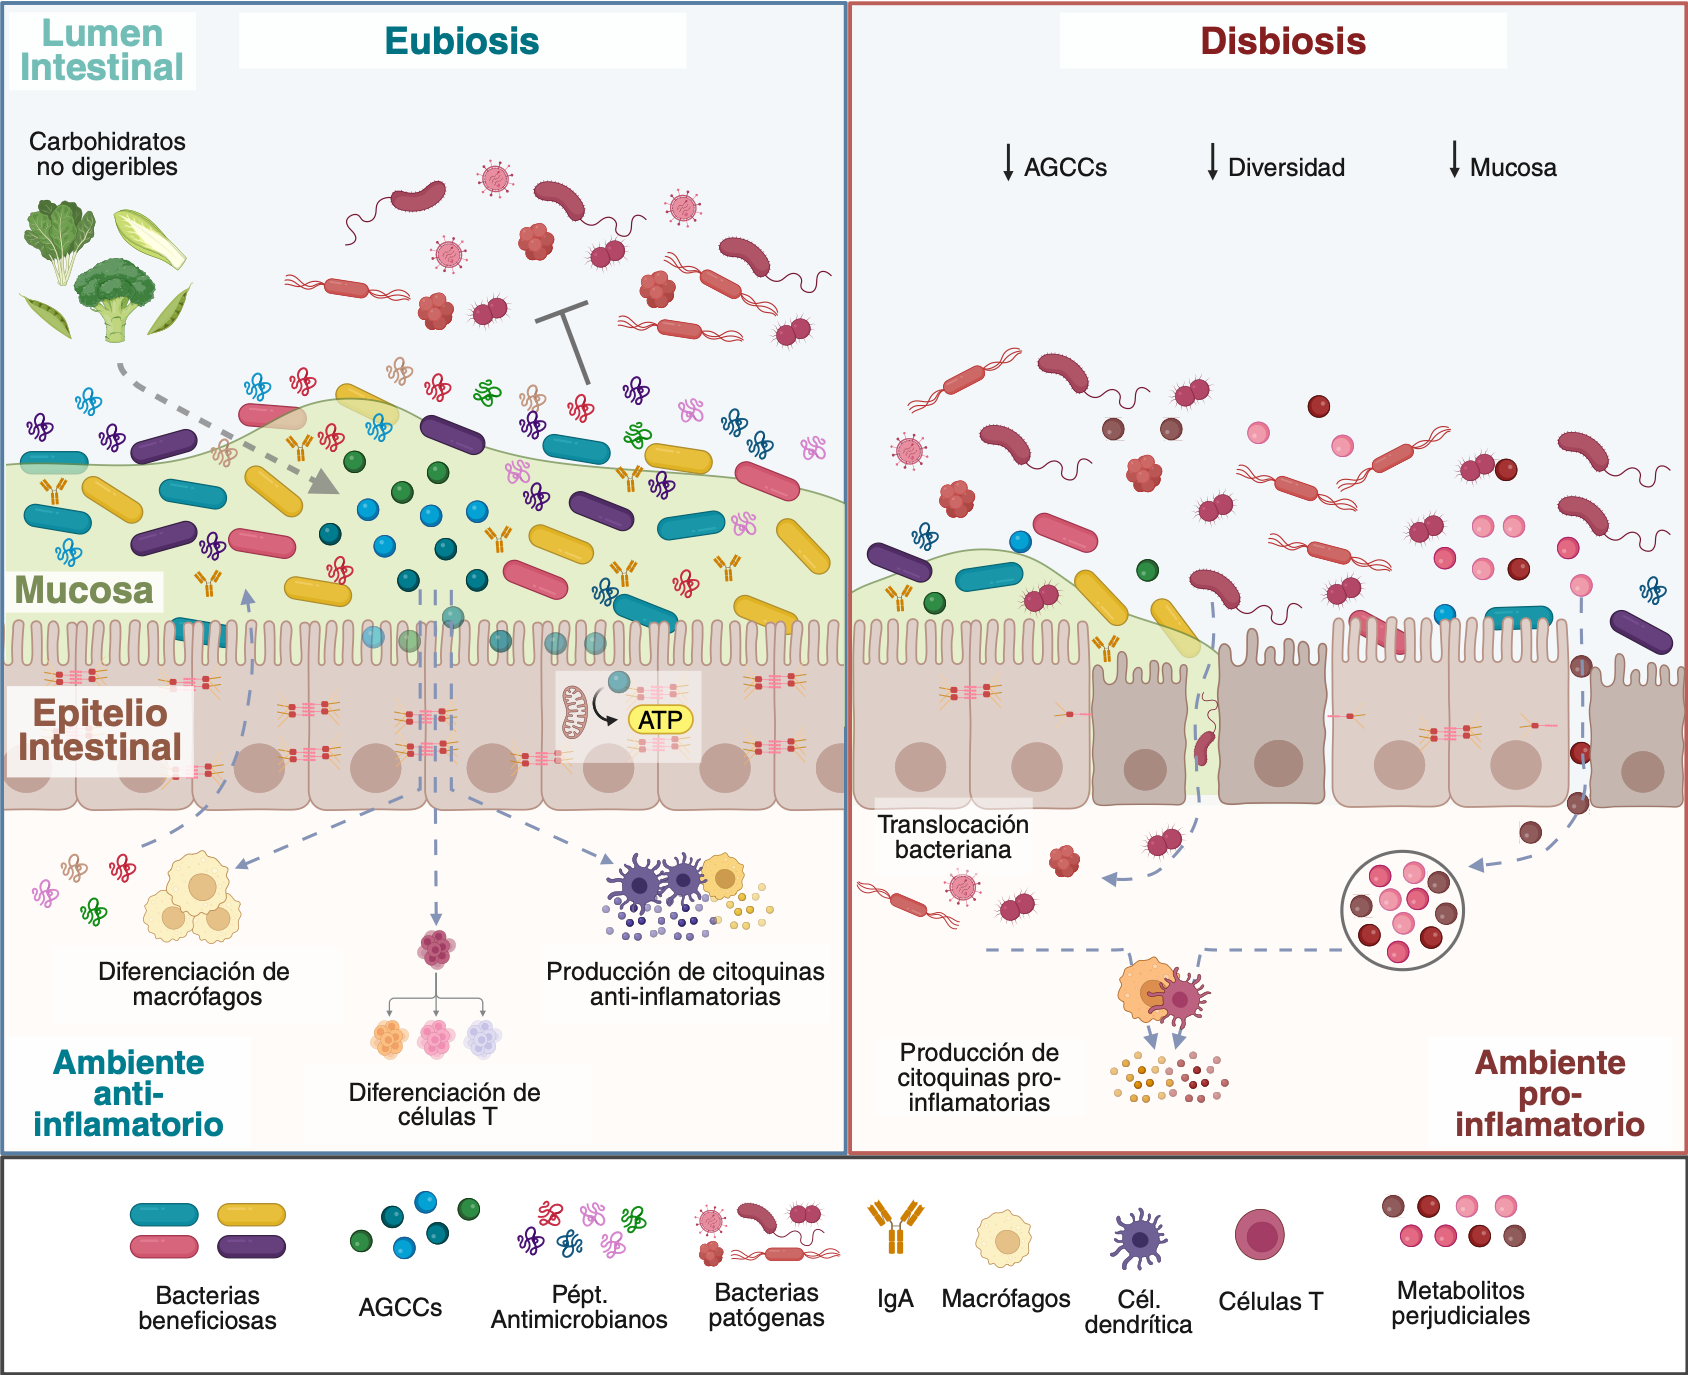
\includegraphics[width=\textwidth]{img/introduction/05_Microbioma_Intestinal.png}
    \caption[Eubiosis y disbiosis intestinal]{\textbf{Representación de los cambios entre eubiosis y disbiosis intestinal.} En la eubiosis, una diversidad alta y equilibrada contribuye a un ambiente antiinflamatorio mediante la producción de AGCCs y citoquinas antiinflamatorias. En la disbiosis, la reducción de AGCCs y la disminución de la diversidad en favor de patógenos, pueden llevar a una inflamación intestinal con tanslocación basteriana y producción de citoquinas proinglamatorias; alterando la integridad del epitelio intestinal. Imagen creada con BioRender \cite{biorender2025}.}
    \label{fig:gut}
\end{figure}

%%% Enfermedades microbioma intestinal %%%

Este estado inflamatorio puede desempeñar un papel primordial en enfermedades como la enfermedad inflamatoria intestinal (EII), el síndrome del intestino irritable (SII), cáncer colorrectal (CCR) e incluso diabetes \cite{fan2021gut, bielka2022role}. La EII, que abarca la enfermedad de Crohn y la colitis ulcerosa, se caracteriza por una disminución de Firmicutes beneficiosos y un aumento de Proteobacterias patógenas, lo que lleva a una inflamación crónica \cite{frank2007molecular}.

El SII implica niveles reducidos de \textit{Lactobacillus} y \textit{Bifidobacterium}, esenciales para la salud intestinal \cite{carding2015dysbiosis}. En trastornos metabólicos como la obesidad y el síndrome metabólico (SM), una proporción alterada de Firmicutes a Bacteroidetes afecta al equilibrio energético y la deposición de grasa \cite{turnbaugh2006obesity}. El CCR también se ha asociado con cambios microbianos específicos, notablemente aumentos en \textit{Fusobacterium nucleatum}, \textit{Escherichia coli} y \textit{Bacteroides fragilis}, sugiriendo que ciertos microbios pueden influir en la carcinogénesis \cite{castellarin2012fusobacterium}.

En la DT1 se observa, por ejemplo, un incremento de bacterias pertenecientes al género \textit{Bacteroides}, destacándose especies como \textit{Bacteroides dorei} y \textit{Bacteroides vulgatus}, incluso antes de la seroconversión de los autoanticuerpos, lo cual sugiere un rol potencial en el desarrollo autoinmune. Paralelamente, se reporta una disminución en la abundancia de bacterias beneficiosas, tales como \textit{Lactobacillus}, \textit{Bifidobacterium}, \textit{Faecalibacterium prausnitzii} y otros productores de butirato, cuya reducción podría contribuir a la disrupción de la barrera intestinal y a la activación de respuestas inflamatorias que favorecen la destrucción de células \textit{beta} pancreáticas \cite{bielka2022role, mejia2015diet, zheng2018gut}. Estudios en modelos animales y en cohortes de niños han corroborado estos hallazgos, asociando una menor diversidad microbiana y cambios en la composición con la aparición de autoanticuerpos y la progresión de la DT1 \cite{bielka2022role, han2018gut}.

Por otro lado, en la DT2 se identifica una disbiosis caracterizada por la reducción de bacterias productoras de butirato (como \textit{Faecalibacterium prausnitzii}, \textit{Roseburia intestinalis} y \textit{Eubacterium rectale}) y un aumento relativo de patógenos oportunistas y ciertos miembros del filo Bacteroidetes, lo que se ha relacionado con la endotoxemia, la inflamación crónica y la resistencia a la insulina. Adicionalmente, se han descrito alteraciones en la proporción entre Firmicutes y Bacteroidetes, además del enriquecimiento de clases como \textit{Betaproteobacteria}, que se correlacionan positivamente con niveles de glucosa en plasma y marcadores de disfunción metabólica \cite{bielka2022role, huda2021modulating}.

No obstante, a pesar de estos importantes avances, el campo del microbioma intestinal enfrenta desafíos críticos. La falta de estandarización en las metodologías de muestreo, extracción y análisis limita la reproducibilidad y comparabilidad entre estudios a gran escala. Además, el mayor reto es establecer la causalidad y no solo la asociación: se requiere la integración de estudios multiómicos, cohortes longitudinales y ensayos de intervención controlados para desarrollar modelos predictivos robustos y terapias de modulación que sean verdaderamente trasladables y personalizadas en la práctica clínica.


\subsubsection{El Microbioma Vaginal}

Un microbioma vaginal sano se caracteriza por una alta dominancia de bacterias del género \textit{Lactobacillus} (como \textit{Lactobacillus crispatus}, \textit{Lactobacillus jensenii}, etc.), como se observa en la Figura \ref{fig:vaginal}. Estas bacterias desempeñan un papel crucial en la protección del entorno vaginal debido a su capacidad para producir ácido láctico, lo que mantiene un pH ácido, generalmente entre 3.8 y 4.5. Este ambiente ácido es fundamental para inhibir el crecimiento de patógenos oportunistas y mantener la homeostasis \cite{hickey2012understanding}. Además de su función en la acidez, los \textit{Lactobacillus} producen peróxido de hidrógeno, una sustancia con propiedades antimicrobianas que ayuda a inhibir el crecimiento de bacterias patógenas. También actúan mediante la secreción de bacteriocinas, pequeñas proteínas o péptidos que inhiben el crecimiento de bacterias patógenas al adherirse a sus membranas celulares, creando poros y provocando la muerte celular \cite{ravel2011vaginal}. Estas acciones contribuyen a preservar la integridad de la barrera epitelial vaginal, ya que los \textit{Lactobacillus} refuerzan las uniones entre las células epiteliales, previniendo la invasión de patógenos. Al interactuar con las células del sistema inmunitario, también modulan el sistema inmune local, estimulando la producción de moléculas señalizadoras que fortalecen la respuesta inmune. Esto contribuye a mantener un estado inflamatorio equilibrado, protegiendo contra infecciones sin inducir una inflamación excesiva, asegurando así un entorno protector y saludable para la función reproductiva \cite{chen2021female}.

%%% Microbioma Vaginal en Disbiosis %%%

En contraposición, la disbiosis del microbioma vaginal (Figura \ref{fig:vaginal}) se manifiesta a través de una disminución significativa en la proporción de bacterias del género \textit{Lactobacillus} y un aumento en la diversidad microbiana, lo cual, a diferencia del microbioma intestinal, resulta perjudicial. Este desequilibrio facilita la proliferación de bacterias anaerobias como \textit{Gardnerella vaginalis} o \textit{Atopobium vaginae}. Estas especies bacterianas alteran la composición y funcionalidad del microbioma, conduciendo a la formación de \textit{biofilms} bacterianos. Estos \textit{biofilms} son comunidades microbianas que se adhieren a la superficie de las células vaginales y están rodeadas por una matriz protectora, lo que hace que las bacterias sean más resistentes a los antibióticos y a la respuesta inmune del anfitrión. Esto complica el tratamiento y favorece la persistencia de la infección, afectando negativamente la integridad de la barrera epitelial \cite{saraf2021vaginal}. Además, en un estado de disbiosis, el pH vaginal se eleva debido a la disminución en la producción de ácido láctico, creando un ambiente propicio para que los organismos patógenos se establezcan y proliferen dentro de estos \textit{biofilms}. La reducción en la producción de peróxido de hidrógeno y bacteriocinas compromete las defensas antimicrobianas naturales, aumentando el riesgo de infecciones y desencadenando una respuesta inflamatoria exacerbada.

\begin{figure}[h]
    \centering
    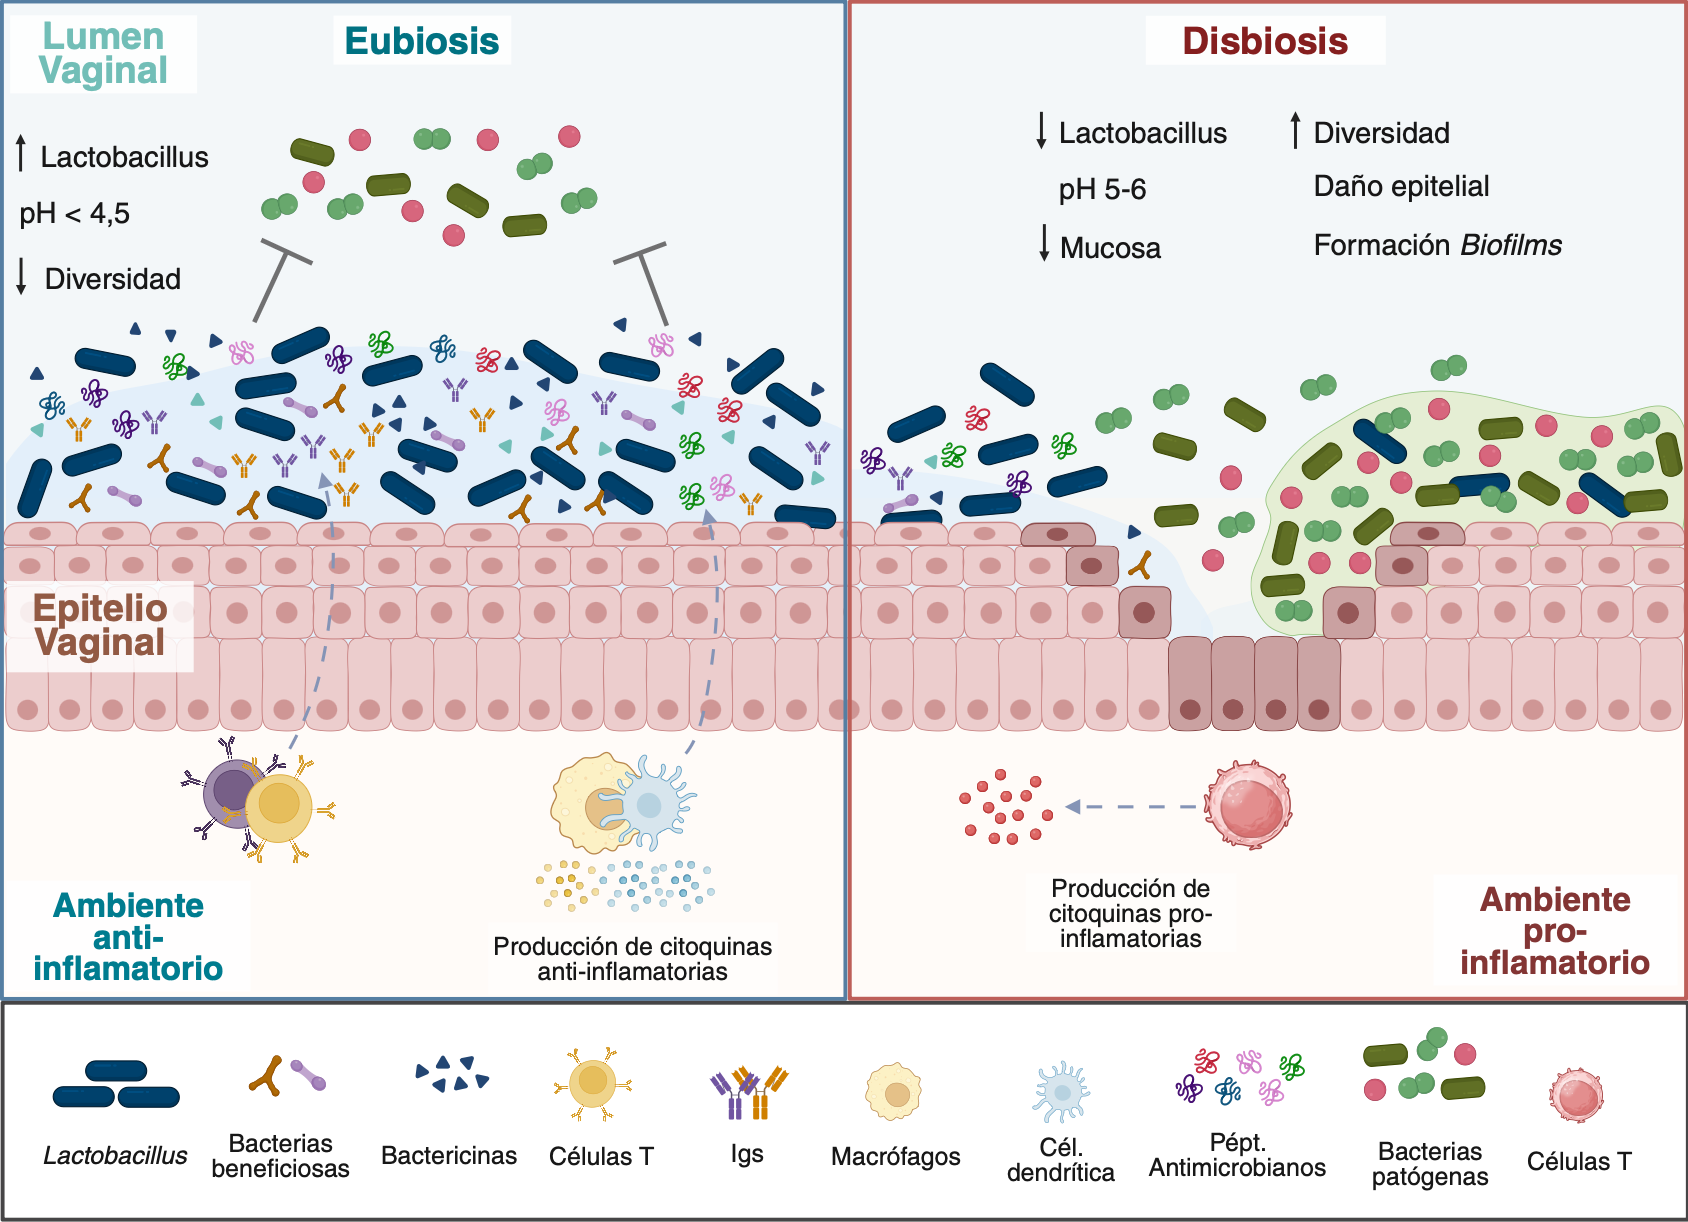
\includegraphics[width=\textwidth]{img/introduction/06_Microbioma_Vaginal.png}
    \caption[Eubiosis y disbiosis vaginal]{\textbf{Representación de los cambios entre eubiosis y disbiosis en el ambiente vaginal.} En la eubiosis, una alta presencia de \textit{Lactobacillus} y un pH menor a 4.5 promueven un ambiente antiinflamatorio con producción de citoquinas antiinflamatorias. En la disbiosis, la disminución de \textit{Lactobacillus} y el aumento del pH a 5-6 pueden provocar un ambiente proinflamatorio, daño epitelial, formación de \textit{biofilms} y producción de citoquinas proinflamatorias. Imagen creada con BioRender \cite{biorender2025}.}
    \label{fig:vaginal}
\end{figure}


%%% Enfermedades microbioma vaginal %%%

Una de las afecciones más comunes relacionadas con la disbiosis vaginal es la VB. Esta enfermedad se caracteriza por una alteración profunda en la microbiota vaginal, donde se produce un marcado descenso de los \textit{Lactobacillus} dominantes, particularmente \textit{Lactobacillus crispatus}, y un aumento concomitante de especies anaeróbicas. Estudios han demostrado que, en mujeres afectadas, la proporción de \textit{Lactobacillus} se reduce drásticamente (de aproximadamente 79\% en mujeres sanas a menos del 20\% en casos de vaginosis), mientras que se observa un incremento de \textit{Lactobacillus iners}, que no confiere la misma protección \cite{chen2021female, ceccarani2019diversity}. Asimismo, se ha documentado la presencia elevada de microorganismos como \textit{Gardnerella vaginalis}, \textit{Atopobium vaginae} y especies del género \textit{Prevotella}, que, como ya se ha comentado, desempeñan un papel central en la formación de \textit{biofilms} en la superficie del epitelio vaginal y en la alteración del pH. Esto se relaciona con los síntomas clínicos típicos de esta enfermedad, como una descarga más grisácea o el mal olor \cite{abou2022bacterial, vitali2015vaginal}. Además, se han identificado otros anaerobios relevantes en la VB, como \textit{Mobiluncus spp.}, \textit{Mycoplasma hominis}, \textit{Sneathia spp.} y diversas bacterias asociadas a VB (\textit{BVAB 1–3}), que en conjunto contribuyen a un ecosistema complejo y polimicrobiano, caracterizado por una respuesta inflamatoria local exacerbada y una mayor resistencia al tratamiento convencional \cite{onderdonk2016human, martin2016vaginal}.

Además, la inflamación crónica puede dañar aún más la barrera epitelial y aumentar la susceptibilidad a infecciones recurrentes y complicaciones a largo plazo \cite{chen2021female, lev2022vaginal}. Las infecciones por hongos son comúnmente causadas por el sobrecrecimiento de especies de \textit{Candida} \cite{sobel2007vulvovaginal}. Es importante destacar que los cambios en el microbioma vaginal están vinculados con el parto prematuro, donde los niveles reducidos de \textit{Lactobacillus} y el aumento de \textit{Mycoplasma} y \textit{Ureaplasma} pueden activar vías inflamatorias que contribuyen a resultados adversos en el embarazo \cite{gudnadottir2022vaginal}.


A pesar de estos conocimientos detallados, la aplicación terapéutica sigue enfrentando retos significativos. Aún es necesario desarrollar herramientas de diagnóstico que permitan la identificación rápida y precisa de los subtipos de disbiosis (no solo en la VB), así como formular estrategias de intervención (probióticos y tratamientos con fagos) que superen la resistencia conferida por los biofilms y logren una colonización estable y duradera de \textit{Lactobacillus} protectores.

%% Párrafo conector a Composicionalidad %%

El estudio de los distintos nichos microbianos, como el intestinal y el vaginal, pone de manifiesto cómo el equilibrio entre las especies que los habitan es crucial para la salud. A través de la secuenciación, se obtienen datos sobre la abundancia relativa de estos microorganismos, lo que nos permite cuantificar y comparar estos perfiles microbianos. Sin embargo, es fundamental comprender que estos datos no representan el número absoluto de microorganismos, sino una proporción de la comunidad. Esta característica inherente los define como datos composicionales, un aspecto clave que debe ser considerado en cualquier análisis estadístico posterior, ya que el aumento de un taxón puede simplemente ser el resultado de la disminución de otro.


\subsection{Composicionalidad}

Como se ha comentado en la sección anterior, la homeostasis de un individuo depende de las fluctuaciones en la composición de las especies que forman parte de un nicho microbiano. El análisis del microbioma, a través de la secuenciación, revela la naturaleza composicional de estos datos. Esto significa que los datos no son conteos absolutos, sino abundancias relativas de cada taxón dentro de una muestra \cite{busato2023compositionality}.

Los equipos de secuenciación generan un número finito de lecturas por muestra. Debido a que este número total es fijo, los datos resultantes se normalizan para que sumen una constante (por ejemplo, 1 o 100\%). Esto convierte a cada muestra en un sistema cerrado, donde las abundancias son interdependientes. En consecuencia, el aumento en la proporción de un taxón debe compensarse matemáticamente con una disminución en la de otros, sin importar si sus números absolutos han cambiado o no \cite{gloor2017microbiome}. Una analogía simple es imaginar la comunidad microbiana como un gráfico circular. Cada sector representa un grupo microbiano diferente. Si un sector se expande, los demás deben contraerse para que el círculo permanezca del mismo tamaño. Esta perspectiva es crucial porque nos obliga a ver los conteos microbianos no como entidades independientes, sino como partes de un ecosistema interconectado, donde cualquier cambio observado es fundamentalmente relativo.

Este escenario de suma fija tiene implicaciones significativas: un aparente aumento en la proporción de un organismo no siempre indica una proliferación real. Podría simplemente reflejar una mayor representación relativa en comparación con otros miembros de la comunidad que han disminuido. Comprender este marco composicional nos permite apreciar la naturaleza dinámica del microbioma, enfatizando las diferencias proporcionales y la idea de que un cambio en un componente afecta a todo el ecosistema. Por lo tanto, para evaluar el equilibrio de una comunidad microbiana, es imperativo considerar todos los taxones de manera colectiva \cite{gloor2017microbiome}. Esta perspectiva es vital para interpretar los cambios entre estados de salud y enfermedad. La disbiosis no se trata solo del aumento o la disminución de un solo taxón, sino de una alteración global en el perfil de abundancias relativas. Por ejemplo, un aparente sobrecrecimiento de una especie podría ser, en realidad, un reflejo de la reducción desproporcionada de otra, lo que subraya la importancia de analizar las interacciones ecológicas subyacentes en lugar de enfocarse en conteos individuales \cite{gloor2016s, vandeputte2017quantitative}.

En resumen, aunque el análisis de datos composicionales presenta desafíos estadísticos que se abordan con técnicas especializadas, la comprensión de este concepto nos recuerda que el microbioma es un ecosistema de abundancias relativas finamente equilibrado. Esta es una perspectiva fundamental para entender tanto su dinámica funcional como sus respuestas a perturbaciones.


%% Párrafo conector a Biomarcadores %%

La capacidad de analizar estos cambios a través de datos de secuenciación composicionales nos permite ir más allá de la mera descripción de la comunidad microbiana. La clave radica en identificar perfiles de composición microbiana o firmas metagenómicas que se correlacionan de manera consistente con estados de enfermedad. Estos patrones, o biomarcadores basados en el microbioma, representan candidatos con un potencial para el diagnóstico, la predicción de enfermedades e incluso la evaluación de la respuesta a tratamientos.

\subsection{Biomarcadores}

% Introducción a los Biomarcadores

Un biomarcador se define como una característica biológica objetiva y cuantificable que refleja el estado de procesos fisiológicos normales, patológicos o la respuesta a intervenciones terapéuticas. Los biomarcadores más utilizados suelen ser moléculas, genes, proteínas, metabolitos u otros componentes biológicos. Estos permiten cuantificar cambios en los organismos que, de otro modo, pasarían desapercibidos a simple vista durante la observación clínica \cite{strimbu2010biomarkers}.

Existen tres categorías fundamentales de biomarcadores, las cuales se distinguen según su función clínica: biomarcadores diagnósticos, biomarcadores pronósticos y biomarcadores predictivos. Los biomarcadores diagnósticos se utilizan para la detección y confirmación de la presencia de una enfermedad. Los biomarcadores pronósticos, por su parte, proporcionan información sobre la evolución probable de una enfermedad, permitiendo la predicción de la progresión de la enfermedad y la supervivencia del paciente. Finalmente, los biomarcadores predictivos anticipan la respuesta de un paciente a un tratamiento específico, lo que permite la personalización de las terapias \cite{strimbu2010biomarkers}.

% Biomarcadores en el Microbioma

La complejidad y dinámica del microbioma lo posicionan como una fuente emergente de biomarcadores con un gran potencial. Estudios recientes demuestran que las variaciones en su composición y funcionalidad pueden correlacionarse con la patogénesis de enfermedades inflamatorias, metabólicas, autoinmunes y ciertos tipos de cáncer, lo que sugiere que patrones microbianos específicos pueden ser utilizados como biomarcadores \cite{hajjo2022unlocking, ayakdacs2023microbiota, duttagupta2023gut, carr2025personalized, eslami2025microbiota}. A modo de ejemplo, se han asociado comunidades microbianas específicas con la progresión del CCR \cite{wirbel2019meta, wang2023fusobacterium, conde2024multispecies} y del cáncer pancreático \cite{kartal2022faecal, nagata2022metagenomic, pourali2024microbiome}. De manera similar, en enfermedades digestivas como la EII y el SII, se han identificado patrones microbianos que actúan como biomarcadores diagnósticos y pronósticos \cite{mousa2024gut, meade2023gut, metwaly2022microbiome}. En las enfermedades metabólicas, como la diabetes, las alteraciones en el microbioma intestinal también se han vinculado con la progresión de la enfermedad, sugiriendo su papel en desequilibrios metabólicos \cite{metwaly2022microbiome, gao2022cross, rold2024identifying}.

Estos trabajos ejemplifican cómo la convergencia de metodologías avanzadas en biología molecular, secuenciación y análisis computacional está sentando las bases para una nueva era en la que los biomarcadores del microbioma se integrarán en la práctica clínica para la toma de decisiones más informadas y precisas.

A pesar del potencial de los biomarcadores del microbioma, su identificación y validación presentan importantes desafíos metodológicos, técnicos y estadísticos. La complejidad del ecosistema microbiano, junto con su variabilidad temporal y la influencia de factores externos como la dieta y el uso de antibióticos, complican la estandarización y reproducibilidad de los resultados. Además, las diferencias en el procesamiento de las muestras y en las técnicas analíticas utilizadas contribuyen a la heterogeneidad de los datos, dificultando la validación de biomarcadores en estudios independientes. Estos retos requieren un diseño experimental riguroso y cohortes diversificadas para obtener conclusiones fiables y aplicables en la práctica clínica \cite{buytaers2024potential, marcos2021applications}.

Pese a las limitaciones actuales, el futuro de los biomarcadores del microbioma es prometedor. Las innovaciones en secuenciación de alto rendimiento, análisis metagenómico y herramientas computacionales están facilitando la identificación de firmas microbianas específicas para desarrollar estrategias terapéuticas personalizadas. Al mismo tiempo, la realización de estudios longitudinales y el uso de modelos \textit{in silico} están mejorando nuestra comprensión de la interacción dinámica entre el anfitrión y su microbioma, lo que incrementará la precisión en la predicción de riesgos y la eficacia de los tratamientos. Estos avances apuntan a superar los desafíos actuales y abrir nuevas vías en la medicina personalizada.


%% Parrafo conector con la siguiente sección %%

A lo largo de estas secciones, se ha explorado cómo el microbioma humano constituye un ecosistema dinámico y complejo, cuyo equilibrio y desequilibrio están íntimamente ligados a la salud. También se ha comprendido que los datos generados a partir de su secuenciación son de naturaleza composicional, lo que presenta desafíos inherentes para su análisis. La búsqueda de biomarcadores a partir de este tipo de datos requiere la aplicación de herramientas especializadas. Para transformar los perfiles microbianos en información clínicamente relevante, es indispensable recurrir a métodos y técnicas computacionales avanzadas. Estas herramientas no solo permiten el preprocesamiento y la exploración de los datos, sino que también son cruciales para la identificación de patrones y, en última instancia, la extracción de firmas microbianas que puedan tener un impacto real en el diagnóstico y tratamiento de enfermedades. Las siguientes secciones se centrarán en detallar estas técnicas y cómo se aplican en la investigación del microbioma.



%%%%%%%%%%%%%%%%%         Técnicas computacionales              %%%%%%%%%%%%%%%%%%%%%%
\section{Métodos y técnicas Computacionales}

En este apartado se hará una descripción de las técnicas computacionales utilizadas durante el desarrollo de esta Tesis Doctoral. La sección se ha dividido en 4 subsecciones: Preprocesamiento, Análisis descriptivos del microbioma, Técnicas de \textit{Machine Learning} y Técnicas de reducción de la dimensionalidad.


\subsection{Preprocesamiento}

El análisis de datos de secuenciación de 16S rRNA comienza con una fase de preprocesamiento para garantizar la fiabilidad de los resultados. Este proceso es crucial para transformar las lecturas de secuenciación crudas en datos taxonómicos estructurados, eliminando artefactos y secuencias de baja calidad que podrían generar resultados espurios. En esencia, este paso sienta las bases para todos los análisis posteriores.

\subsubsection{Obtención de conteos taxonómicos}

La mayoría de las plataformas de secuenciación generan archivos en formato FASTQ, que contienen tanto la secuencia de nucleótidos como su información de calidad. Estos archivos se caracterizan por contener cuatro líneas por cada lectura secuenciada (Figura \ref{fig:FASTQ}). La primera línea comienza con el símbolo @, seguido de un identificador único para la secuencia. La segunda línea contiene la secuencia de nucleótidos. La tercera línea empieza con el símbolo +, y puede repetir el identificador o estar vacía. La cuarta línea proporciona las puntuaciones de calidad para cada nucleótido, utilizando un código ASCII que refleja la calidad de las lecturas.

\begin{figure}[h]
    \centering
    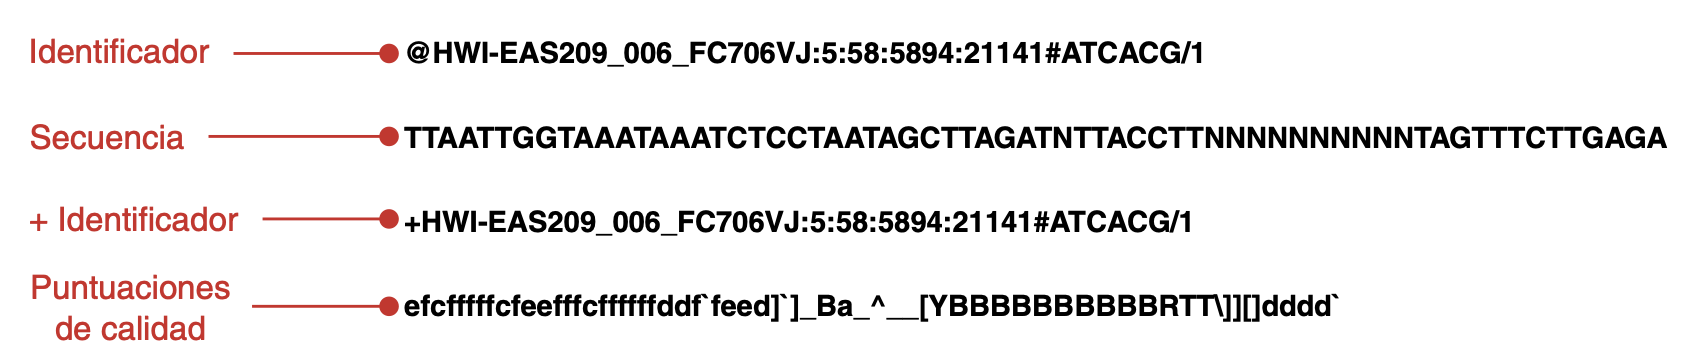
\includegraphics[width=\textwidth]{img/introduction/FASTQ.png}
    \caption[Formato FASTQ]{\textbf{Formato FASTQ y una breve explicación de cada línea del formato.} Imagen creada con BioRender \cite{biorender2025}.}
    \label{fig:FASTQ}
\end{figure}


El flujo de trabajo utilizado en esta Tesis Doctoral para el preprocesamiento de secuencias de 16S rRNA incluye varios pasos críticos (Figura \ref{fig:preprocessing}). En una primera etapa, se realiza un control de calidad de las secuencias, empleando herramientas como FastQC \cite{andrews2010} para evaluar métricas como la calidad de las lecturas, el contenido de guanina-citosina y la posible presencia de \textit{primers} o secuencias contaminantes. Si se detectan \textit{primers} residuales, estos se eliminan utilizando Cutadapt \cite{martin2011cutadapt}, una herramienta diseñada para cortar secuencias no deseadas de manera eficiente.


Una vez que las secuencias han pasado el control de calidad, la siguiente fase es la generación de ASVs y la posterior asignación taxonómica. Para la generación de ASVs a partir de las secuencias, se ha optado por usar el enfoque DADA2 \cite{callahan2016dada2}, que consta de varias fases críticas para asegurar la generación precisa de ASVs. Primero, se procede con el filtrado y recorte de las secuencias, donde se eliminan aquellas de baja calidad y se ajustan sus longitudes para mejorar la precisión en la fase de inferencia. Después, se realiza una fase de aprendizaje de errores, una fase distintiva de DADA2 en la que el software estima las tasas de error específicas de la secuenciación para diferenciar las verdaderas variantes biológicas de los artefactos. A continuación, se efectúa la inferencia de ASVs, modelando esos errores para distinguir las secuencias biológicas reales. Una vez inferidas las ASVs, se lleva a cabo la eliminación de quimeras, comprobando y suprimiendo las secuencias artificiales generadas durante la amplificación por PCR. Posteriormente, se construye la tabla de conteos de ASVs y se procede con su asignación taxonómica mediante bases de datos de referencia. En el caso de la presente Tesis Doctoral, se utilizó la base de datos de SILVA \cite{quast2012silva}.

Finalmente, después de realizar la asignación taxonómica, se construye en R un objeto phyloseq \cite{mcmurdie2013phyloseq} con la tabla de ASVs, la tabla taxonómica y los metadatos de las muestras. Este objeto es el punto de partida de todos los análisis posteriores.

\begin{figure}[!h]
    \centering
    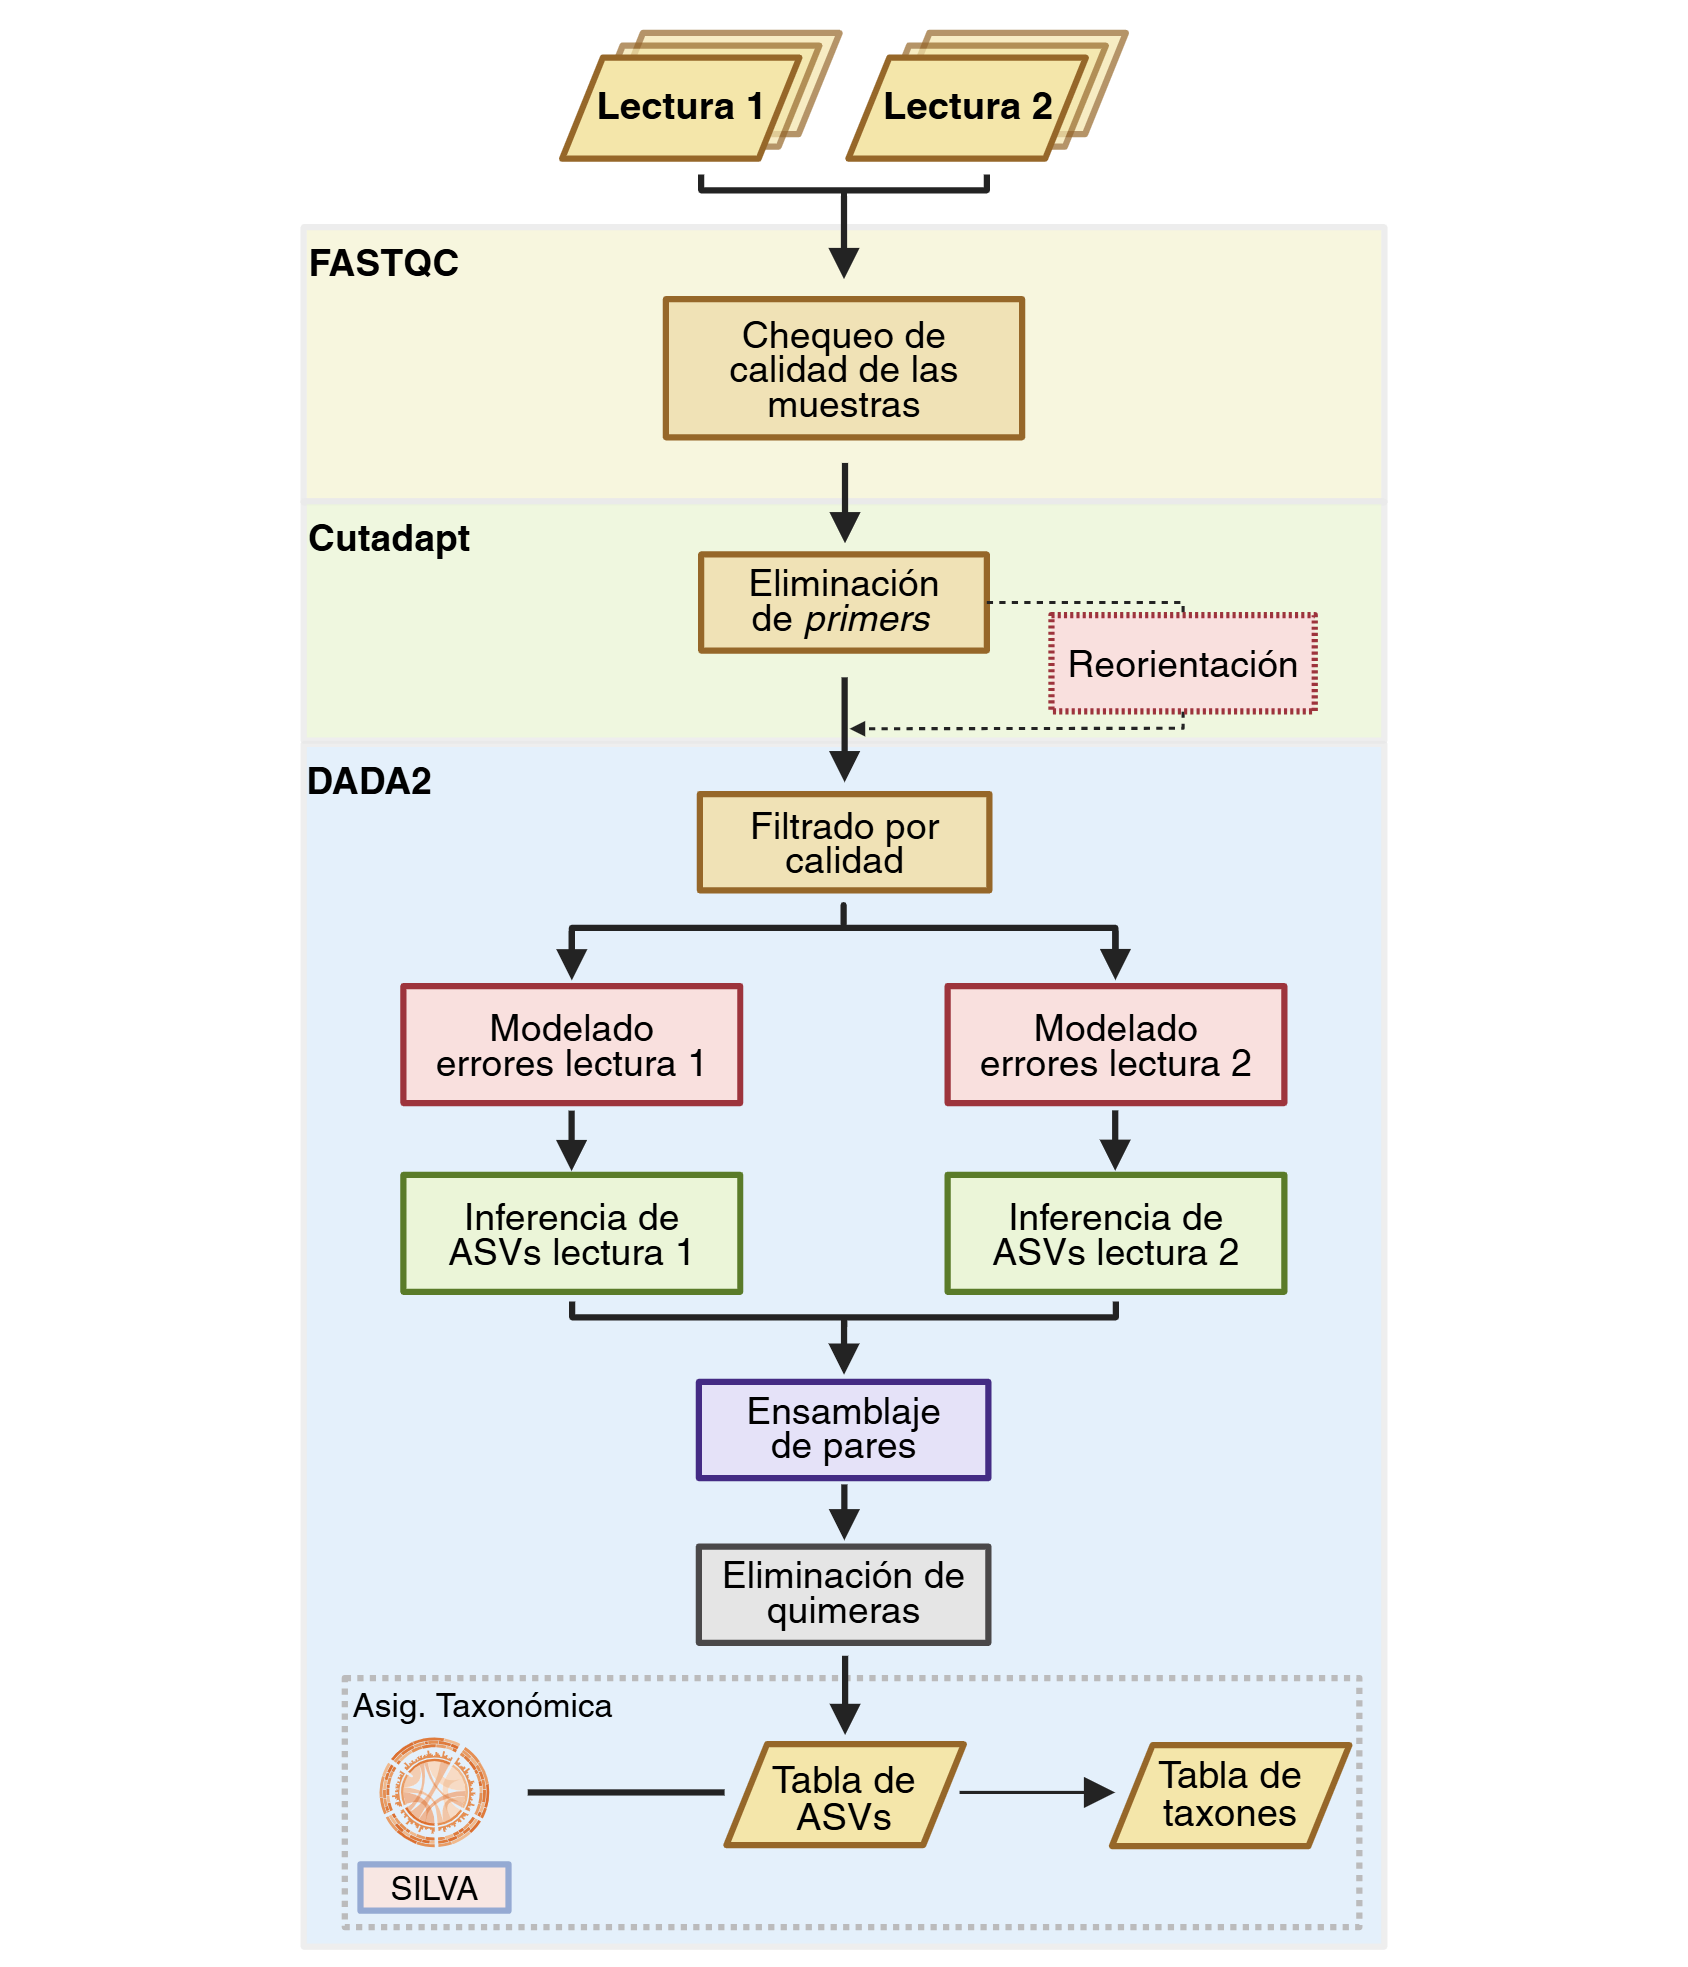
\includegraphics[width=0.9\textwidth]{img/introduction/Preprocesado.png}
    \caption[Flujo de trabajo del preprocesado]{\textbf{Flujo de trabajo para el procesamiento de datos de secuenciación de 16S rRNA} utilizando FASTQC, Cutadapt y DADA2. El proceso incluye un control de calidad inicial, la eliminación de \textit{primers}, el preprocesado y, finalmente, la asignación taxonómica de las ASVs inferidas. Imagen creada con BioRender \cite{biorender2025}.}
    \label{fig:preprocessing}
\end{figure}


\subsubsection{Caracterización de los conteos taxonómicos}

Tras la inferencia de ASVs y su correspondiente asignación taxonómica, es fundamental preprocesar estos conteos taxonómicos para mitigar las diferencias en la profundidad de secuenciación entre las muestras. Actualmente, existen dos métodos principales para el preprocesamiento de estos conteos: la rarefacción y el enfoque composicional \cite{willis2019rarefaction, gloor2017microbiome}. Estos métodos difieren en cómo manejan la variabilidad inherente en la profundidad de secuenciación y la naturaleza relativa de los conteos observados, cada uno con ventajas y limitaciones que influyen en los análisis e inferencia estadística posteriores \cite{hong2022rarefy, peterson2023analysis}.

\paragraph{Rarefacción}

La rarefacción es una técnica que submuestrea aleatoriamente las lecturas de cada muestra para que todas tengan la misma profundidad. Este método se aplica comúnmente en el análisis de datos de 16S rRNA porque iguala la profundidad de secuenciación entre muestras, permitiendo pruebas estadísticas sencillas y comparaciones de diversidad \cite{willis2019rarefaction}. Su clara ventaja radica en su simplicidad y facilidad de implementación, lo que también facilita el cálculo de métricas de diversidad \textit{alfa} y \textit{beta} bajo condiciones de muestreo consistentes. Sin embargo, la rarefacción tiene inconvenientes significativos; entre otros: descarta lecturas que exceden el límite elegido, lo que lleva a una pérdida de información valiosa, reduciendo el poder estadístico y potencialmente disminuyendo la capacidad de detectar verdadera variación biológica. Esta pérdida de información puede comprometer la fiabilidad de los resultados \cite{peterson2023analysis, schloss2024waste}.

\paragraph{Enfoque composicional}

El enfoque composicional considera los datos del microbioma como proporciones de un todo, es decir, los conteos de taxones son inherentemente relativos. En lugar de submuestrear, este método aplica transformaciones estadísticas especializadas, como transformaciones de razón logarítmica. Las transformaciones más comunes son: la transformación logarítmica centrada (CLR), la transformación logarítmica aditiva (ALR) y la transformación logarítmica isométrica (ILR). Estas transformaciones tienen en cuenta adecuadamente esta interdependencia y naturaleza relativa \cite{gloor2017microbiome}.

La principal ventaja del enfoque composicional es que preserva toda la información de los datos, evitando la pérdida inherente a la rarefacción. A pesar de requerir un modelado estadístico más complejo para tratar problemas como los ceros, esta estrategia ofrece una mayor robustez y consistencia en la identificación de taxones diferenciales y en la interpretación de la estructura de la comunidad \cite{peterson2023analysis, gloor2016s}.

Dada su capacidad para tratar adecuadamente la naturaleza relativa de los datos del microbioma, el enfoque composicional es considerado por la literatura reciente como el método más apropiado, mejorando la precisión de la inferencia taxonómica y la detección de cambios biológicamente relevantes \cite{peterson2023analysis, schloss2024waste}. Por esta razón, los datos de la presente Tesis Doctoral han sido tratados bajo el enfoque composicional.

%% Párrafo conector a A.Descriptivos %%

Una vez que los datos del microbioma han sido preprocesados correctamente, se procede a su análisis. La siguiente etapa se enfoca en la caracterización descriptiva del microbioma. Estos análisis iniciales tienen como objetivo determinar la composición y la estructura de las comunidades microbianas, lo que facilita la formulación de hipótesis de investigación y sirve de base para la aplicación de métodos más complejos.

\subsection{Análisis descriptivos del microbioma}

Tras el preprocesamiento de las secuencias, realizar análisis descriptivos del microbioma es un paso habitual. Entre ellos destacan la diversidad \textit{alfa}, que evalúa la diversidad dentro de las muestras, y la diversidad \textit{beta}, que investiga las diferencias entre comunidades microbianas. Además de las métricas de diversidad, otro enfoque habitual es el análisis de abundancia diferencial, que se utiliza para identificar taxones cuya abundancia relativa difiere entre dos o más condiciones. 

\subsubsection{Diversidad \textit{alfa}}

La diversidad \textit{alfa} evalúa la diversidad dentro de una muestra individual o comunidad microbiana (Figura \ref{fig:Alfa_Beta}). El objetivo es capturar la complejidad interna del microbioma mediante la cuantificación del número de taxones (riqueza) y su distribución de abundancia relativa (uniformidad) dentro de una única muestra \cite{finotello2018measuring}. Los índices más comunes para evaluar la diversidad \textit{alfa} son aquellos que integran tanto la riqueza como la uniformidad, como los índices de Shannon y Simpson \cite{hagerty2020empirically}.

\begin{figure}[h]
    \centering
    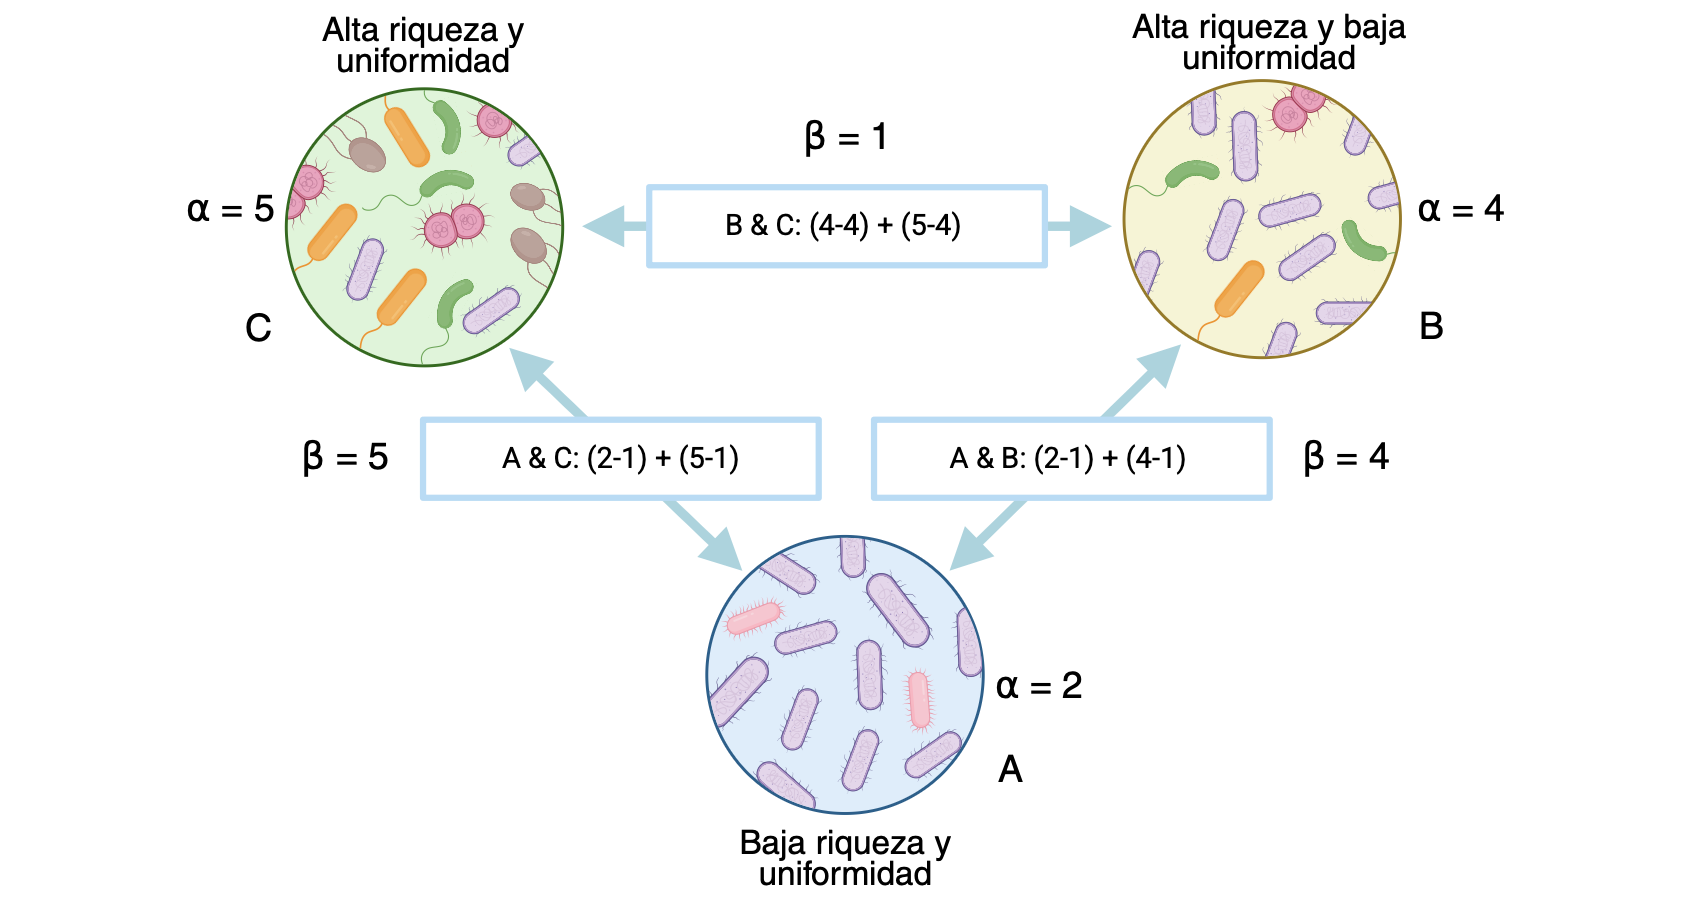
\includegraphics[width=\textwidth]{img/introduction/Alfa_Beta.png}
    \caption[\textit{Alfa} y \textit{Beta} diversidad]{\textbf{Representación esquemática de la diversidad \textit{alfa} y \textit{beta} en comunidades microbianas.}
La diversidad \textit{alfa} se ilustra como la composición interna de cada comunidad (A, B, C), mientras que la diversidad \textit{beta} se representa como las diferencias entre pares de comunidades, calculadas a partir de la presencia o ausencia de taxones compartidos. Imagen creada con BioRender \cite{biorender2025}.}
    \label{fig:Alfa_Beta}
\end{figure}


El índice de Shannon mide la incertidumbre al predecir la especie de un taxón elegido al azar de la comunidad. Este índice considera tanto la riqueza de especies como la distribución de las abundancias, ofreciendo una medida equilibrada que refleja no solo cuántos taxones hay, sino también cómo están distribuidos los individuos entre ellos \cite{finotello2018measuring}. Su formulación es la siguiente:

\begin{equation}
H = -\sum_i \left( p_i \cdot \ln(p_i) \right)
\end{equation}
\myequations{Índice de Shannon}
\begin{itemize}
\item Donde $p_i$ denota la proporción de taxones que pertenecen a la $i$-ésima especie en la muestra.
\end{itemize}

Valores altos indican mayor incertidumbre, lo que significa una mayor diversidad. En cambio, valores bajos sugieren menor incertidumbre y, por lo tanto, menor diversidad. Debido a la naturaleza logarítmica del índice de Shannon, se garantiza que las especies raras tengan menor impacto en el valor total de diversidad, en comparación con las especies dominantes. Esto captura la heterogeneidad intrínseca de la comunidad y minimiza el peso excesivo de taxones poco frecuentes. Sin embargo, este índice es sensible al tamaño de la muestra y la profundidad de secuenciación.

Por otro lado, el índice de Simpson se enfoca en la probabilidad de que dos taxones elegidos al azar pertenezcan a la misma especie. Su formulación es la siguiente:

\begin{equation}
D = \sum_i \left( p_i^2 \right)
\end{equation}
\myequations{Índice de Simpson}
\begin{itemize}
\item Donde $p_i$ denota la proporción de taxones que pertenecen a la $i$-ésima especie en la muestra.
\end{itemize}


La medida complementaria (1 – D) se utiliza para una interpretación más intuitiva, donde los valores más altos indican mayor diversidad. Este índice se centra en las especies abundantes, ya que al elevar al cuadrado las proporciones, se destaca la influencia de los taxones comunes frente a los raros. Aunque es robusto frente a errores de muestreo y fácil de interpretar en términos de dominancia, puede pasar por alto la importancia de especies raras que podrían ser ecológicamente significativas \cite{finotello2018measuring}.


El cálculo de la diversidad \textit{alfa} ofrece múltiples beneficios. Primero, indica la complejidad del ecosistema al mostrar el número de especies y su distribución uniforme. Un valor alto sugiere una comunidad microbiana más robusta y resistente, mientras que un valor bajo puede indicar disbiosis o el dominio de pocos taxones, lo que podría predisponer a enfermedades \cite{hagerty2020empirically}.

\subsubsection{Diversidad \textit{beta}}

A diferencia de la diversidad \textit{alfa}, la diversidad \textit{beta} se enfoca en las diferencias en la composición taxonómica entre múltiples comunidades (Figura \ref{fig:Alfa_Beta}). Este tipo de análisis busca identificar patrones de disimilitud entre comunidades, los cuales podrían estar relacionados con variaciones en las características del anfitrión, la salud o los tratamientos \cite{kers2022power}. En la práctica, la diversidad \textit{beta} se evalúa utilizando una variedad de métricas de disimilitud o distancia. Medidas cuantitativas, como la disimilitud de Bray–Curtis, y métricas cualitativas, como el índice de Jaccard, son las más utilizadas actualmente \cite{finotello2018measuring}.

Por un lado, el índice de Bray–Curtis, al ser una medida cuantitativa, calcula la disimilitud entre dos comunidades basándose en datos de abundancia de especies. Su formulación es la siguiente:

\begin{equation}
BC_{ij} = \frac{\sum |x_{ik} - x_{jk}|}{\sum (x_{ik} + x_{jk})}
\end{equation}
\myequations{Índice de Bray–Curtis}
\begin{itemize}
\item Donde $x_{ik}$ y $x_{jk}$ representan la abundancia de la $k$-ésima especie en las muestras i y j. 
\end{itemize}

El valor resultante varía entre 0 y 1, donde 0 indica que las dos comunidades son idénticas y 1 señala una disimilitud completa. La medida de Bray–Curtis es particularmente sensible a las diferencias en las especies abundantes, ya que suma las diferencias absolutas en los conteos entre especies y se normaliza por la abundancia total, capturando así las sutilezas en los cambios de composición de la comunidad impulsados por los taxones dominantes \cite{kers2022power}.

Por otro lado, el índice de Jaccard, al ser una medida cualitativa, se calcula en función de la presencia o ausencia de taxones en cada muestra, en lugar de sus abundancias. El índice de disimilitud de Jaccard se deriva dividiendo el número de taxones no compartidos entre dos muestras por el total de taxones presentes en la unión de ambas muestras:

\begin{equation}
J = 1 - \frac{a}{a + b + c}
\end{equation}
\myequations{Índice de Jaccard}
\begin{itemize}
\item Donde $a$ es el número de especies presentes en ambas comunidades, $b$ es el número de especies presentes solo en la comunidad 1 y $c$ es el número de especies presentes solo en la comunidad 2.
\end{itemize}

El resultado es un valor que varía de 0 a 1, donde 0 indica que las dos comunidades son idénticas y 1 señala una disimilitud completa. Gracias a su enfoque en la información de presencia o ausencia, este índice tiende a estar menos influenciado por taxones abundantes y, por lo tanto, es particularmente adecuado para comparaciones en las que los taxones raros proporcionan percepciones biológicas críticas \cite{kers2022power}. 
 
Evaluar la diversidad \textit{beta} permite determinar si los grupos de muestras forman comunidades distintas. Por ejemplo, diferencias significativas en la diversidad \textit{beta} entre individuos sanos y enfermos pueden indicar una reestructuración de la comunidad microbiana asociada con una determinada patología \cite{finotello2018measuring}.



\subsubsection{Análisis de abundancia diferencial}


Los análisis de abundancia diferencial son fundamentales para identificar taxones microbianos cuyas abundancias cambian significativamente entre distintos grupos, como individuos sanos y enfermos \cite{kleine2021data} (Figura \ref{fig:DA}). Este tipo de análisis complementa la visión general de la diversidad al señalar taxones específicos que pueden estar asociados con un fenotipo o una condición particular.

\begin{figure}[h]
    \centering
    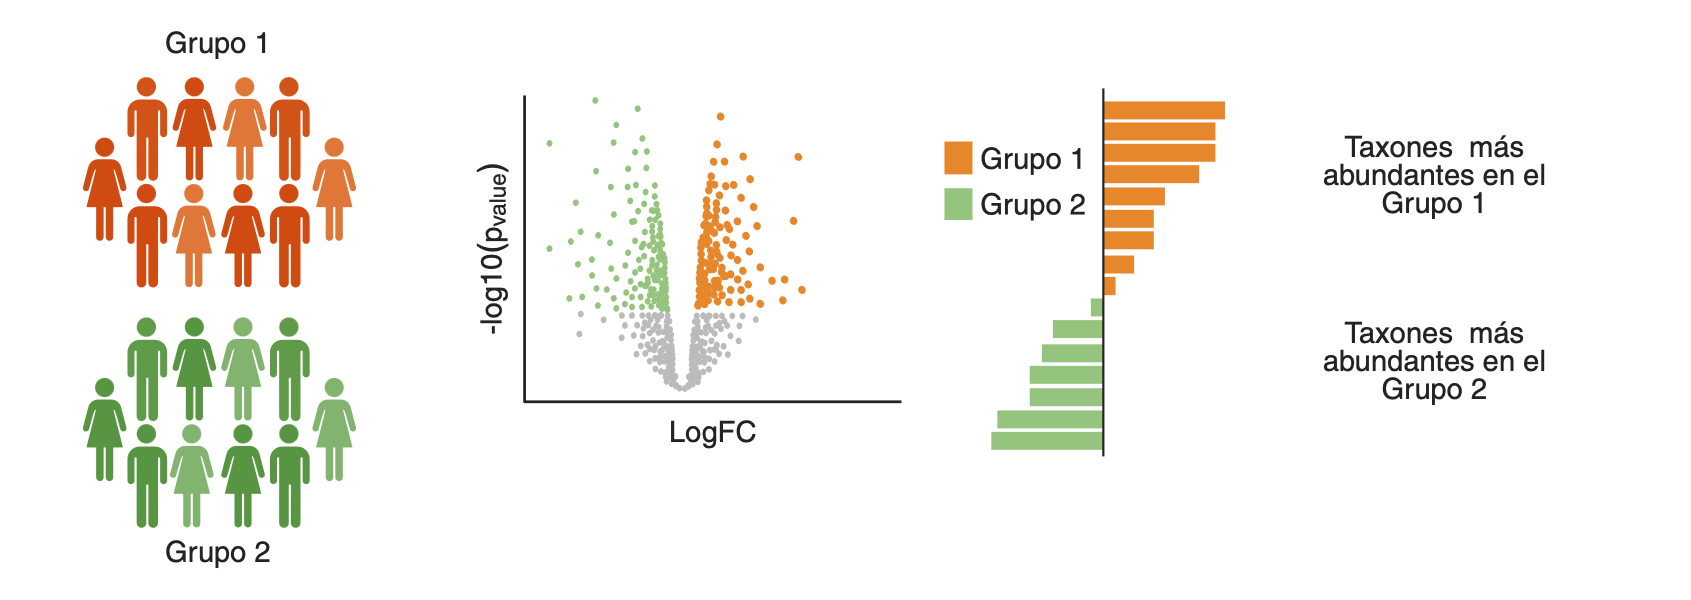
\includegraphics[width=\textwidth]{img/introduction/DA.png}
    \caption[Análisis de abundacia diferencial]{\textbf{Representación de un análisis de abundancia diferencial.} A la izquierda se ilustra cada grupo. En el centro, el gráfico volcán muestra para cada taxón el cambio de abundancia ($\log\mathrm{FC}$) frente a la significación ($-\log_{10}(p)$): valores de $\log\mathrm{FC}$ positivos indican mayor abundancia en el Grupo 1 y negativos en el Grupo 2. A la derecha, las barras horizontales resumen los taxones con mayor efecto ($ \lvert \log_{2}\mathrm{FC} \rvert $) y mayor evidencia estadística en cada grupo, ordenados por magnitud. Imagen creada con BioRender \cite{biorender2025}.}
    \label{fig:DA}
\end{figure}

Este tipo de análisis permite identificar características microbianas específicas que podrían asociarse con fenotipos clínicos o procesos biológicos. La base conceptual de estos métodos proviene del análisis de expresión diferencial del transcriptoma, donde se busca identificar genes cuya actividad varía entre grupos de estudio. Métodos como DESeq \cite{love2014moderated}, edgeR \cite{robinson2010edger} y limma \cite{ritchie2015limma} sentaron las bases para el desarrollo de enfoques especializados, adaptados a las particularidades de los datos de microbioma.

Entre estas particularidades destacan las ya comentadas en secciones anteriores: su estructura composicional, la prevalencia de conteos nulos, la alta variabilidad entre individuos y fracciones de muestreo desiguales. Como respuesta, han surgido varios enfoques que intentan lidiar con estas características, los cuales han sido utilizados a lo largo del desarrollo de esta Tesis Doctoral.


\textbf{\textit{Multivariate Association with Linear Models}}

\textit{Multivariate Association with Linear Models} (MaAsLin2) \cite{mallick2021multivariable} representa un enfoque más convencional para el análisis de abundancia diferencial. Su objetivo es integrar diversas covariables mediante un modelo lineal multivariable flexible. En lugar de utilizar correcciones explícitas para los sesgos composicionales o las diferencias en las fracciones de muestreo, MaAsLin2 aplica procedimientos de normalización estándar para abordar las diferencias en tamaño de biblioteca y profundidad de secuenciación.

El proceso analítico de MaAsLin2 inicia con el preprocesamiento de los datos. Los perfiles de abundancia, generalmente expresados en conteos, se normalizan mediante métodos como la normalización por suma total (TSS), lo que convierte los datos en proporciones relativas. Posteriormente, se aplican transformaciones (ya sean logarítmicas o transformaciones de raíz cuadrada arco seno) para estabilizar la varianza y adecuar los datos a los supuestos de los modelos lineales.

Una vez preprocesados, los datos son analizados a través de modelos lineales multivariables. En este enfoque, cada característica microbiana se modela de manera univariada, pero de forma simultánea se incluyen múltiples variables predictoras. De esta forma, se puede evaluar el efecto independiente de cada variable sobre la abundancia de la característica en estudio, obteniéndose coeficientes que reflejan la magnitud y dirección de la asociación.

Las pruebas estadísticas que acompañan al ajuste de cada modelo permiten determinar la significancia de los coeficientes, y se aplican métodos de corrección por pruebas múltiples (como el procedimiento de Benjamini-Hochberg) para controlar la tasa de falsos descubrimientos.


\textbf{\textit{Linear Models for Differential Abundance Analysis}}

\textit{Linear Models for Differential Abundance Analysis} (LinDA) \cite{zhou2022linda} es un enfoque que aborda la naturaleza composicional del microbioma, los problemas derivados de distintas profundidades de secuenciación y el problema de inflación de ceros. Se fundamenta en la transformación logarítmica de los datos de abundancia relativa y la aplicación de modelos de regresión lineal ordinaria para estimar asociaciones entre las abundancias de los taxones y covariables de interés.

Este método comienza aplicando una transformación CLR a los conteos taxonómicos, convirtiendo las relaciones multiplicativas entre los conteos de taxones en relaciones aditivas en una escala logarítmica. Este procedimiento normaliza los datos (eliminando el efecto de diferentes profundidades de secuenciación) y preserva la información relativa de la composición microbiana. Esto permite suponer que, tras la transformación, los datos siguen una distribución lognormal.

Una característica clave de LinDA es su paso explícito para la corrección de sesgos. Al reconocer que la transformación CLR puede introducir sesgos cuando algunos taxones realmente difieren, LinDA asume que la mayoría de los taxones no cambia entre condiciones experimentales.

Bajo esta premisa de mayoría nula, LinDA ajusta los coeficientes de regresión usando la moda o la mediana para centrar la distribución alrededor de cero bajo la hipótesis nula. Esta corrección se utiliza para ajustar los cambios logarítmicos estimados, reduciendo así los sesgos que podrían alterar las conclusiones estadísticas. Dicha corrección es esencial para que las estimaciones finales reflejen mejor las diferencias biológicas reales, en lugar de artefactos debidos a restricciones composicionales.

Finalmente, LinDA también implementa controles rigurosos de la tasa de falsos descubrimientos, típicamente mediante procedimientos como el de Benjamini-Hochberg, lo que contribuye a la identificación de diferencias verdaderas en abundancia sin sobreestimarlas.

\textbf{\textit{Analysis of Composition of Microbiomes with Bias Correction}}

\textit{Analysis of Composition of Microbiomes with Bias Correction} (ANCOM-BC) \cite{lin2020analysis} es un enfoque que aborda directamente el sesgo introducido por la variabilidad en las fracciones de muestreo. La base de este método radica en el hecho de que los datos obtenidos en estudios de microbioma representan solo una fracción desconocida de la abundancia absoluta presente en el ecosistema, y que dicha fracción varía entre muestras debido a diferencias en el tamaño de la biblioteca y la carga microbiana. Esta variabilidad, si no se corrige, puede conducir a conclusiones erróneas en el análisis de abundancia diferencial.

La metodología se fundamenta en transformaciones logarítmicas que son análogas a las transformaciones de razón logarítmica utilizadas tradicionalmente en el análisis de datos composicionales. Sin embargo, a diferencia de otros enfoques, ANCOM-BC estima explícitamente los sesgos individuales de cada muestra, lo que posibilita la corrección del sesgo inducido por diferencias en las fracciones de muestreo y evita la necesidad de asumir que la mayoría de los taxones no presentan diferencias de abundancias.

Esta corrección se realiza de forma iterativa. Inicialmente, se estiman los efectos de las covariables y el sesgo específico de cada muestra; a continuación, se ajustan los coeficientes estimados mediante técnicas de tipo Expectativa-Maximización o modelos de mezcla gaussiana que permiten aislar y corregir el sesgo. Esta corrección mejora el poder de detectar diferencias reales en la abundancia entre condiciones experimentales.


\textbf{\textit{Analysis of Differential Abundance Taking Sample Variation Into Account}}

\textit{Analysis of Differential Abundance Taking Sample Variation Into Account} (ALDEx2) \cite{fernandes2014unifying} integra la naturaleza composicional de los datos de secuenciación con la variabilidad técnica y biológica inherente a cada muestra.

El proceso inicia con la transformación de los conteos observados en abundancias relativas utilizando un enfoque de muestreo de Monte Carlo. ALDEx2 genera múltiples réplicas de cada muestra extrayéndolas de una distribución de Dirichlet. Esta simulación modela la incertidumbre en las proporciones observadas y captura la variabilidad asociada a distintos factores técnicos y biológicos. De esta forma, en lugar de basarse en estimaciones puntuales, el método aprovecha una distribución de posibles valores de abundancia, lo que permite inferencias estadísticas que incorporan la variación muestral de manera explícita.

Una vez que se generan las réplicas de Monte Carlo, ALDEx2 aplica la transformación CLR a cada vector de abundancias relativas. Esta transformación normaliza los datos (eliminando el efecto de diferentes profundidades de secuenciación) y preserva la información relativa de la composición microbiana.

Sobre los datos transformados, ALDEx2 realiza pruebas estadísticas univariadas para identificar taxones con diferencias significativas entre condiciones experimentales o grupos biológicos. Para esto, se pueden usar pruebas paramétricas, como el test t de Welch, o pruebas no paramétricas, como la de Wilcoxon. Debido a la generación de múltiples réplicas por muestra, se calculan valores de p individuales que luego se promedian, y se aplica la corrección de Benjamini-Hochberg para controlar la tasa de falsos descubrimientos.

Al seleccionar entre estos métodos, se deben considerar varios factores clave. Por un lado, si es crucial obtener estimaciones precisas de las abundancias microbianas absolutas, los enfoques de modelado, como ANCOM-BC o ALDEx2, son los más indicados. Por otro lado, si el conjunto de datos presenta escasez considerable o se necesita robustez frente a valores atípicos (\textit{outliers}), LinDA ofrece ventajas importantes. Por último, en estudios epidemiológicos de gran escala que requieren ajustes multivariables flexibles, la eficiencia computacional y el enfoque multivariable de MaAsLin2 pueden ser muy beneficiosos, aunque su dependencia de la normalización convencional puede dejar algunos efectos composicionales sin resolver.

%% Transición a ML %%

Los análisis descriptivos del microbioma, como los aquí presentados, permiten comprender su estructura, identificar patrones de abundancia y sugerir posibles biomarcadores. Sin embargo, para la construcción de modelos predictivos, la estratificación de pacientes y el descubrimiento de firmas metagenómicas que reflejen la complejidad biológica de los datos, se requiere el uso de técnicas más avanzadas.

\subsection{Técnicas de \textit{Machine Learning}}

El \textit{Machine Learning} (ML) es una rama de la Inteligencia Artificial que se enfoca en extraer conocimiento valioso de conjuntos de datos mediante algoritmos. Este enfoque basado en datos entrena modelos para minimizar errores de predicción y descubrir patrones ocultos \cite{mitchell1997machine}. Las técnicas de ML se clasifican según el nivel de supervisión: aprendizaje supervisado, no supervisado y semisupervisado. Específicamente en clínica, el aprendizaje no supervisado se utiliza para la estratificación de pacientes o la identificación de subgrupos dentro de una patología, mientras que el aprendizaje supervisado se emplea para la clasificación o predicción de pacientes según una patología \cite{bishop2006pattern, deo2015machine}.

El ML se ha convertido gradualmente en un enfoque esencial para el análisis del microbioma, debido a su naturaleza intrínsecamente compleja. Al emplear estas técnicas, es posible explorar el espacio de características del microbioma para identificar patrones y relaciones que no son evidentes a simple vista. Por ejemplo, a través de técnicas de aprendizaje no supervisado, se pueden agrupar muestras en función de la composición microbiana, lo que puede llevar a la identificación de subgrupos dentro de una población con una determinada condición de salud. Asimismo, el aprendizaje supervisado permite la clasificación de estados patológicos en función de los perfiles microbianos individuales. Estas capacidades hacen del ML una herramienta de gran valor para comprender las complejidades del microbioma y su impacto en la salud.

Esta sección aborda los dos tipos de aprendizaje, los diferentes algoritmos utilizados para cada uno de estos enfoques, las estrategias de validación y las medidas de rendimiento empleadas para evaluar los modelos. Sin embargo, antes de profundizar en estos temas, es crucial entender conceptos básicos del ML, como la distinción entre parámetros e hiperparámetros y su importancia en el rendimiento del modelo.


\subsubsection{Modelos de ML y búsqueda de hiperparámetros}

En la resolución de un problema mediante técnicas de ML, es necesario explorar un amplio catálogo de posibilidades para obtener una arquitectura óptima. La arquitectura óptima se refiere al conjunto de configuraciones externas (denominadas hiperparámetros) que maximizan el rendimiento de un modelo, tanto en eficiencia como en capacidad de generalización. Es importante aclarar la diferencia entre parámetro e hiperparámetro de un modelo. Por un lado, los parámetros son los coeficientes internos de un modelo que se entrenan directamente a partir de los datos de entrada mediante una función interna de optimización (transformación interna de los datos de entrada a una salida deseada). Por otro lado, los hiperparámetros son coeficientes externos definidos antes del proceso de aprendizaje; estos controlan el comportamiento, la capacidad, la estructura y las propiedades de convergencia del modelo \cite{feurer2019hyperparameter}.

El ajuste de hiperparámetros comienza con la creación de un espacio de búsqueda, seguido de una estrategia para encontrar la mejor combinación. Las estrategias más comunes son: búsqueda \textit{grid}, aleatoria y heurística.


La búsqueda \textit{grid} es la más elemental, consiste en definir un rango discreto de valores para cada hiperparámetro y evaluar sistemáticamente todas las combinaciones posibles. La mejor combinación es elegida en función de una métrica de rendimiento previamente elegida. Aunque exhaustiva, su principal limitación es el elevado costo computacional, especialmente cuando el espacio de búsqueda es grande.

La búsqueda aleatoria aparece como una alternativa para mitigar la ineficiencia computacional de la búsqueda \textit{grid}. Este método muestrea aleatoriamente valores de una distribución estocástica definida para cada hiperparámetro. Al no evaluar todas las combinaciones, mitiga la ineficiencia de la búsqueda grid, aunque su éxito es probabilístico y puede no converger siempre a la configuración más óptima.

La búsqueda heurística se diferencia de las dos estrategias anteriores en que se basa en la utilización de información de experimentos anteriores para optimizar las pruebas subsecuentes. Es decir, la búsqueda de hiperparámetros se lleva a cabo de manera guiada hasta alcanzar un punto óptimo. Aunque computacionalmente exigente, resulta útil en espacios de búsqueda muy amplios, ya que la búsqueda se dirige hacia el punto óptimo. Sin embargo, existe el riesgo de converger en mínimos locales.

En resumen, un ajuste cuidadoso de los hiperparámetros es esencial para optimizar el equilibrio entre el sesgo y la varianza del modelo. Un modelo bien ajustado es capaz de generalizar y rendir de manera robusta con nuevos datos, evitando tanto el sobreajuste (memorizar el ruido) como el subajuste (no aprender patrones relevantes).


\subsubsection{Aprendizaje no supervisado}

El aprendizaje no supervisado es una rama del ML que explora datos sin etiquetas predefinidas. A diferencia del aprendizaje supervisado, los modelos no se entrenan con ejemplos de entrada y salida, sino que descubren patrones, estructuras o relaciones inherentes a los datos por sí mismos. Las principales aplicaciones de este tipo de aprendizaje incluyen el agrupamiento (\textit{clustering}) para juntar muestras o características similares y la reducción de la dimensionalidad para simplificar datos complejos \cite{bishop2006pattern}.

En el contexto de esta Tesis Doctoral, esta sección se enfoca en las técnicas de \textit{clustering}. La reducción de la dimensionalidad se abordará en una sección posterior, independientemente de si se basa en ML u otra metodología.

El \textit{clustering} es una técnica de ML que divide un conjunto de datos en subgrupos, o \textit{clusters}, donde los elementos de un mismo \textit{cluster} son más similares entre sí que con los del resto. La mayoría de los algoritmos de \textit{clustering} basan sus estratificaciones en el cálculo de distancias, ya que su función principal es cuantificar la similitud o disimilitud entre los elementos (o puntos de datos) que se desean agrupar. Existen múltiples tipos de distancias para medir esta similitud o disimilitud \cite{bishop2006pattern}.

Las técnicas de \textit{clustering} son fundamentales para el análisis del microbioma, ya que permiten abordar la complejidad inherente a estos datos no etiquetados. Al agrupar muestras con perfiles microbianos similares, facilitan el descubrimiento de patrones específicos, como alteraciones en la composición bacteriana, subgrupos de pacientes o variaciones que no serían detectables con otros enfoques. Es crucial notar que, en la investigación de muchas enfermedades complejas, las variables y/o etiquetas clínicas tradicionales a menudo no se alinean completamente con la variabilidad intrínseca capturada por los datos ómicos o del microbioma, pues no logran encapsular toda la heterogeneidad molecular subyacente. Por esta razón, el análisis no supervisado se vuelve indispensable: nos permite, en primer lugar, cuantificar y comprender la variabilidad explicada por los datos del microbioma por sí solos. Solo después de identificar estos subgrupos biológicos, se procede a asociarlos posteriormente con los datos clínicos disponibles (como la severidad de la enfermedad o la respuesta al tratamiento). Esta estrategia es esencial para la búsqueda de posibles biomarcadores microbianos que puedan actuar como indicadores de patologías y para avanzar hacia una estratificación más precisa de los pacientes.

A continuación, se presentan las medidas de distancia más utilizadas, incluyendo la distancia de Aitchison, recomendada para datos composicionales:


% Distancia de Euclidiana
\textbf{Distancia Euclidiana:} es la medida más común y mide la distancia directa entre dos puntos en un espacio n-dimensional. Su formulación es la siguiente:
\begin{equation}
d_{\text{euclidiana}}(\mathbf{x}, \mathbf{y}) = \sqrt{\sum_{i=1}^{n} (x_i - y_i)^2}
\end{equation}
\myequations{Distancia Euclidiana}
\begin{itemize}
\item Donde $x$ e $y$ son vectores que representa un punto en el espacio n-dimensional.
\end{itemize}

% Distancia de Manhattan
\textbf{Distancia de Manhattan:} es la suma de las diferencias absolutas entre las coordenadas de los puntos. Su formulación es la siguiente:
\begin{equation}
d_{\text{manhattan}}(\mathbf{x}, \mathbf{y}) = \sum_{i=1}^{n} |x_i - y_i|
\end{equation}
\myequations{Distancia de Manhattan}
\begin{itemize}
\item Ddonde $x$ e $y$ son vectores que representa un punto en el espacio (n)-dimensional.
\end{itemize}

% Distancia de Aitchison
\textbf{Distancia de Aitchison:} calcula la distancia entre dos composiciones, es decir, entre vectores que representan partes de un todo. Su formulación es la siguiente:
\begin{equation}
d_{\text{aitchison}}(\mathbf{x}, \mathbf{y}) = \sqrt{\sum_{i=1}^{n} \left( \log\left(\frac{x_i}{g(\mathbf{x})}\right) - \log\left(\frac{y_i}{g(\mathbf{y})}\right) \right)^2}
\end{equation}
\myequations{Distancia de Aitchison}
\begin{itemize}
\item Donde: $x$ e $y$ son vectores que representa una composición, es decir, un conjunto de valores que describen proporciones en un contexto específico;  $x_i$ e $y_i$ son las proporciones de los componentes en las composiciones $x$ e $y$; y $g($x$)$ y $g($y$)$  son los valores geométricos de las composiciones $x$ e $y$.
\end{itemize}

A continuación se presentan los algoritmos de \textit{clustering} utilizados en esta Tesis Doctoral.

\paragraph{\textit{Hierarchical clustering}}

El \textit{Hierarchical clustering} (HC) construye una estructura anidada en forma de árbol, o dendrograma, para representar la agrupación de los datos \cite{johnson1967hierarchical}. Este método puede seguir un enfoque aglomerativo (de abajo hacia arriba), donde cada muestra comienza como un \textit{cluster} independiente y va fusionando uno con otro, progresivamente, en \textit{clusters} más grandes según la similitud (Figura \ref{fig:HC}). Alternativamente, se puede optar por un enfoque divisivo (de arriba hacia abajo), donde todas las muestras comienzan en un solo \textit{cluster} y lo dividen iterativamente en \textit{subclusters} más pequeños. 

El algoritmo se basa en métricas de distancia y criterios de enlace para determinar cómo se combinan los grupos. Los principales criterios de enlace son:
\begin{enumerate}
\item Enlace simple: Mínima distancia entre cualquier par de puntos de diferentes \textit{clusters}.

\item Enlace completo: Máxima distancia entre cualquier par de puntos de diferentes \textit{clusters}.

\item Enlace promedio: Promedio de todas las distancias entre los puntos de ambos \textit{clusters}.

\item Método de Ward: Minimiza la suma total de las varianzas dentro de cada \textit{cluster} para mantener la homogeneidad.
\end{enumerate}

Los hiperparámetros clave del HC son la elección de la métrica de distancia y el criterio de enlace. Las principales ventajas de este método son que no requiere especificar el número de \textit{clusters} de antemano y que proporciona una representación visual clara. Sin embargo, su elevado costo computacional limita su escalabilidad a grandes conjuntos de datos y lo hace sensible a los \textit{outliers} y al ruido.


\begin{figure}[h]
    \centering
    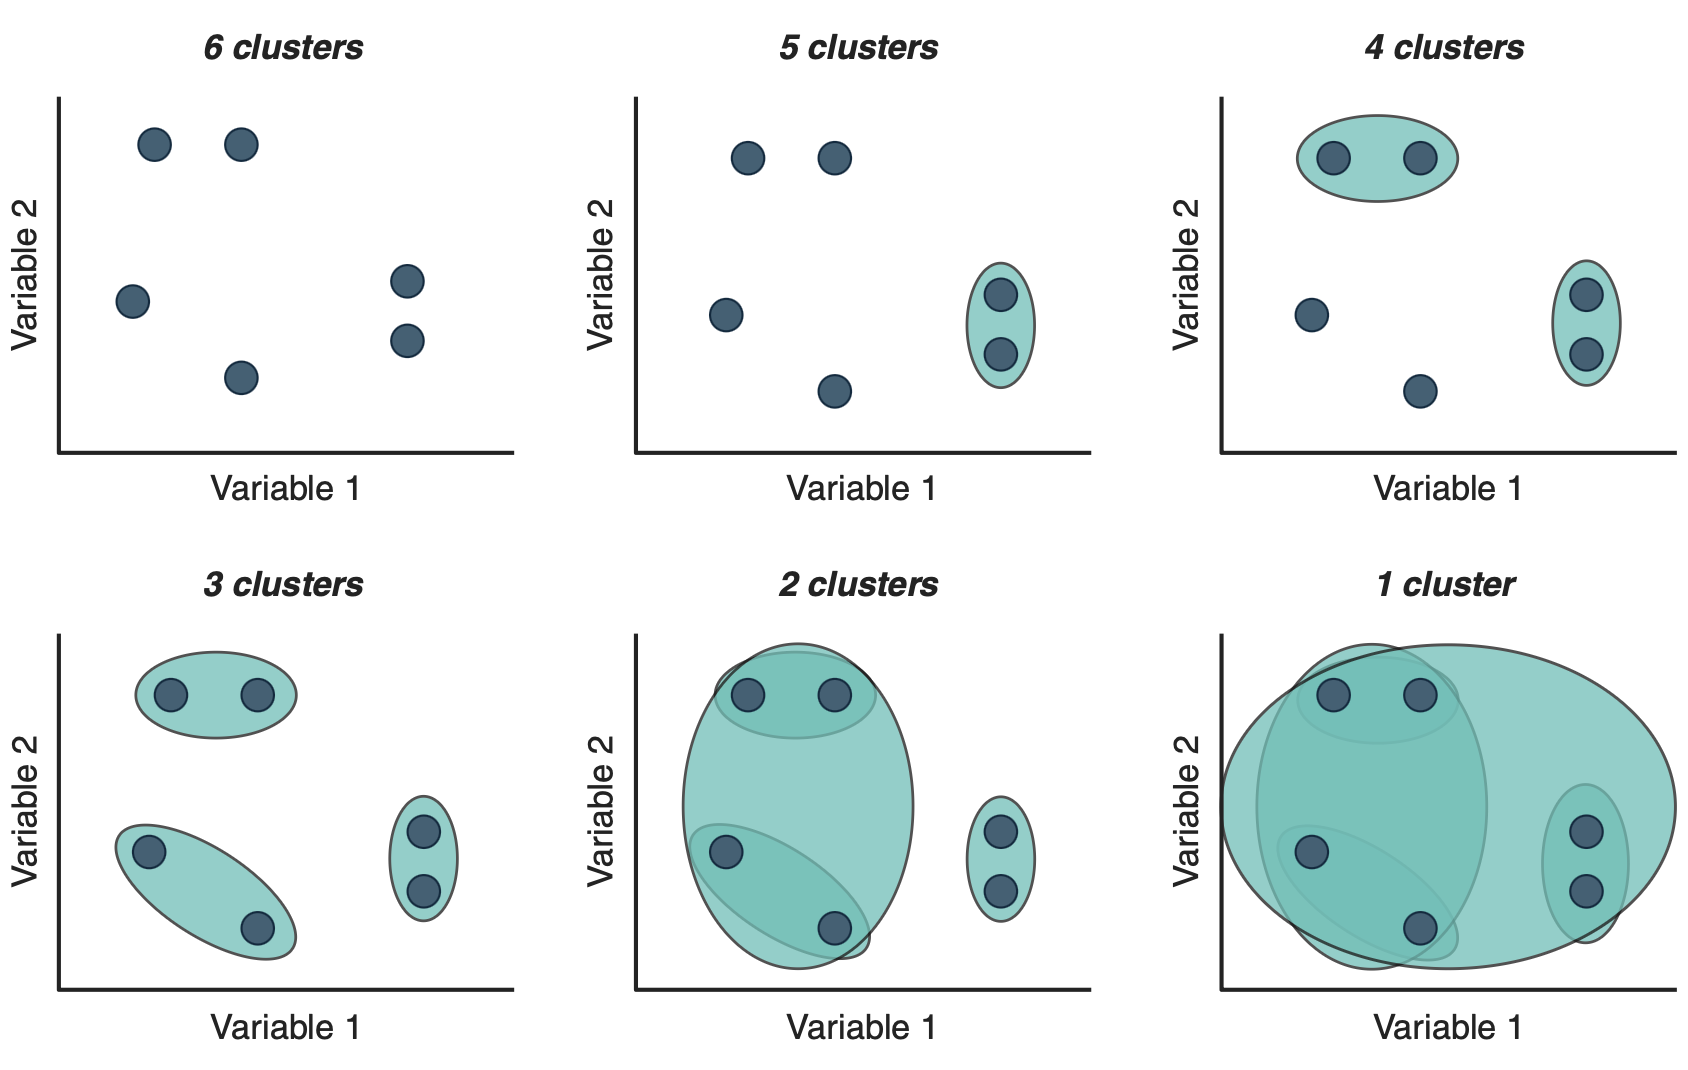
\includegraphics[width=\textwidth]{img/introduction/07_HC.png}
    \caption[\textit{Hierarchical clustering}]{\textbf{Representación del HC utilizando un enfoque aglomerativo.} La imagen muestra como, mediante la combianción de datos, el número de \textit{clusters} se reduce progresivamente desde 6 hasta 1. Cada gráfico ilustra el proceso en diferentes etapas del \textit{clustering} para dos variables. Imagen creada con BioRender \cite{biorender2025}.}
    \label{fig:HC}
\end{figure}


\paragraph{\textit{K-means}}

\textit{K-means} es un algoritmo que divide los datos en un número \textit{k} de \textit{clusters} (especificado por el usuario) al minimizar la suma de las distancias euclidianas al cuadrado entre cada punto y el centroide de su \textit{cluster}. El centroide es el punto que representa el centro de un \textit{cluster} y se calcula como la media de las coordenadas de todos los puntos que lo componen.

Su funcionamiento está representado en la Figura \ref{fig:K-means} y es el siguiente:

\begin{enumerate}
\item Se elige el número deseado de \textit{clusters} (\textit{k}).
\item Se inicializan los centroides, ya sea de forma aleatoria o mediante una métrica específica.
\item Se asigna cada punto al \textit{cluster} con el centroide más cercano. 
\item Se actualizan los centroides recalculando la media de los puntos asignados a cada \textit{cluster}.
\item Los pasos 3 y 4 se repiten hasta que la posición de los centroides cambie mínimamente, lo que indica la convergencia.
\end{enumerate}

Los hiperparámetros clave para \textit{K-means} incluyen el número de \textit{clusters} (\textit{k}), el método de inicialización y el número máximo de iteraciones. Este método es rápido y eficiente para grandes conjuntos de datos, aunque es sensible a la inicialización de los centroides y puede converger en un óptimo local.


\begin{figure}[h]
    \centering
    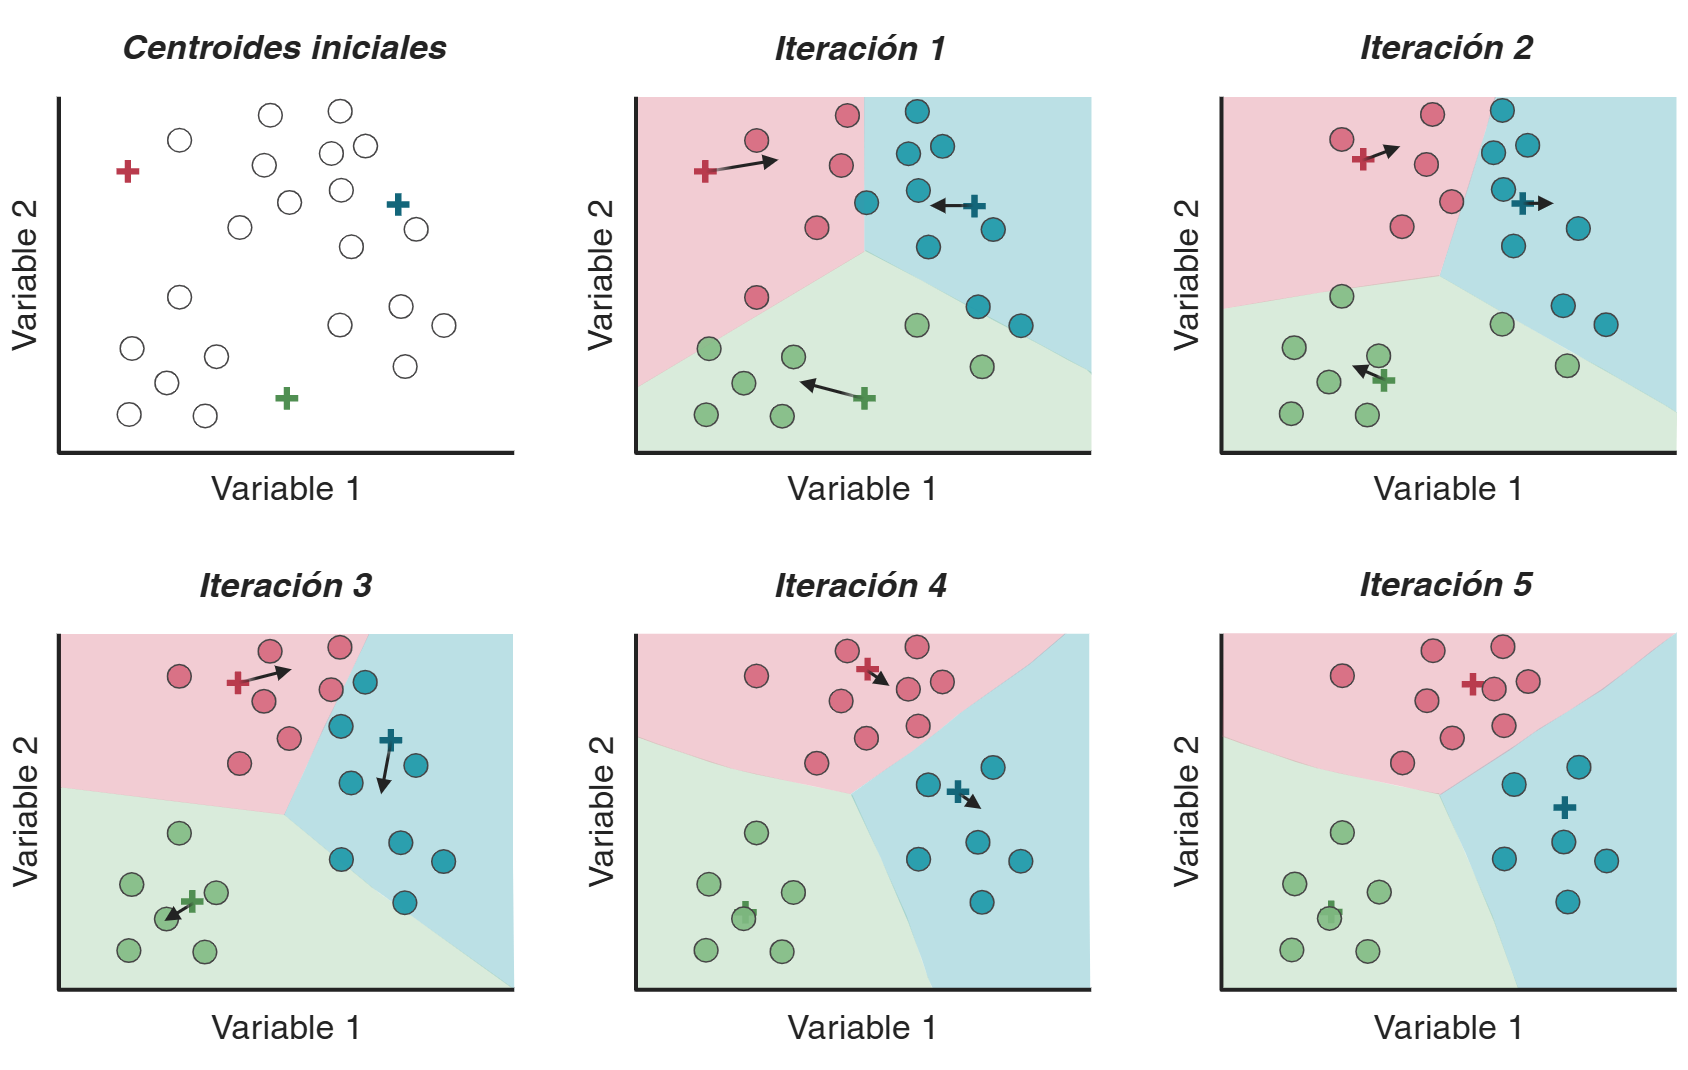
\includegraphics[width=\textwidth]{img/introduction/08_KM.png}
    \caption[\textit{K-means}]{\textbf{Ilustración del algoritmo de \textit{K-means} mostrando el proceso iterativo de agrupamiento.} La imagen presenta desde la selección de centroides iniciales hasta la quinta iteración, destacando cómo los puntos de datos se agrupan alrededor de los centroides que se actualizan en cada iteración para minimizar la varianza dentro de cada \textit{cluster}. Imagen creada con BioRender \cite{biorender2025}.}
    \label{fig:K-means}
\end{figure}


\paragraph{\textit{Partitioning Around Medoids}}

\textit{Partitioning Around Medoids} (PAM) es un algoritmo que surge como alternativa al \textit{K-means}, abordando algunas de las cuestiones de sensibilidad inherentes a \textit{K-means} al usar medoides en lugar de centroides. Un medoide es el punto real dentro de un \textit{cluster} cuya disimilitud total con respecto a todos los demás puntos en el \textit{cluster} es mínima. Por lo tanto, se basa en la minimización de la disimilitud entre los puntos y el medoide del \textit{cluster}, en lugar de la media \cite{rdusseeun1987clustering}.

Su funcionamiento está representado en la Figura \ref{fig:PAM} y es el siguiente:
\begin{enumerate}
\item Se elige un número \textit{k} de medoides iniciales.
\item Se asigna cada punto al medoide más cercano.
\item Se recalculan los medoides para minimizar la disimilitud dentro de cada \textit{cluster}.
\item Los pasos 2 y 3 se repiten que se alcanza la convergencia, generalmente señalada por cambios mínimos en las posiciones de los medoides entre iteraciones.
\end{enumerate}

Los hiperparámetros críticos en PAM son el número de \textit{clusters} iniciales, la inicialización de los medoides y la elección de la métrica de disimilitud. Aunque es más robusto a \textit{outliers} y puede trabajar con distancias no euclidianas, es más lento y computacionalmente más costoso que \textit{K-means}, especialmente con grandes conjuntos de datos.

\begin{figure}[h]
    \centering
    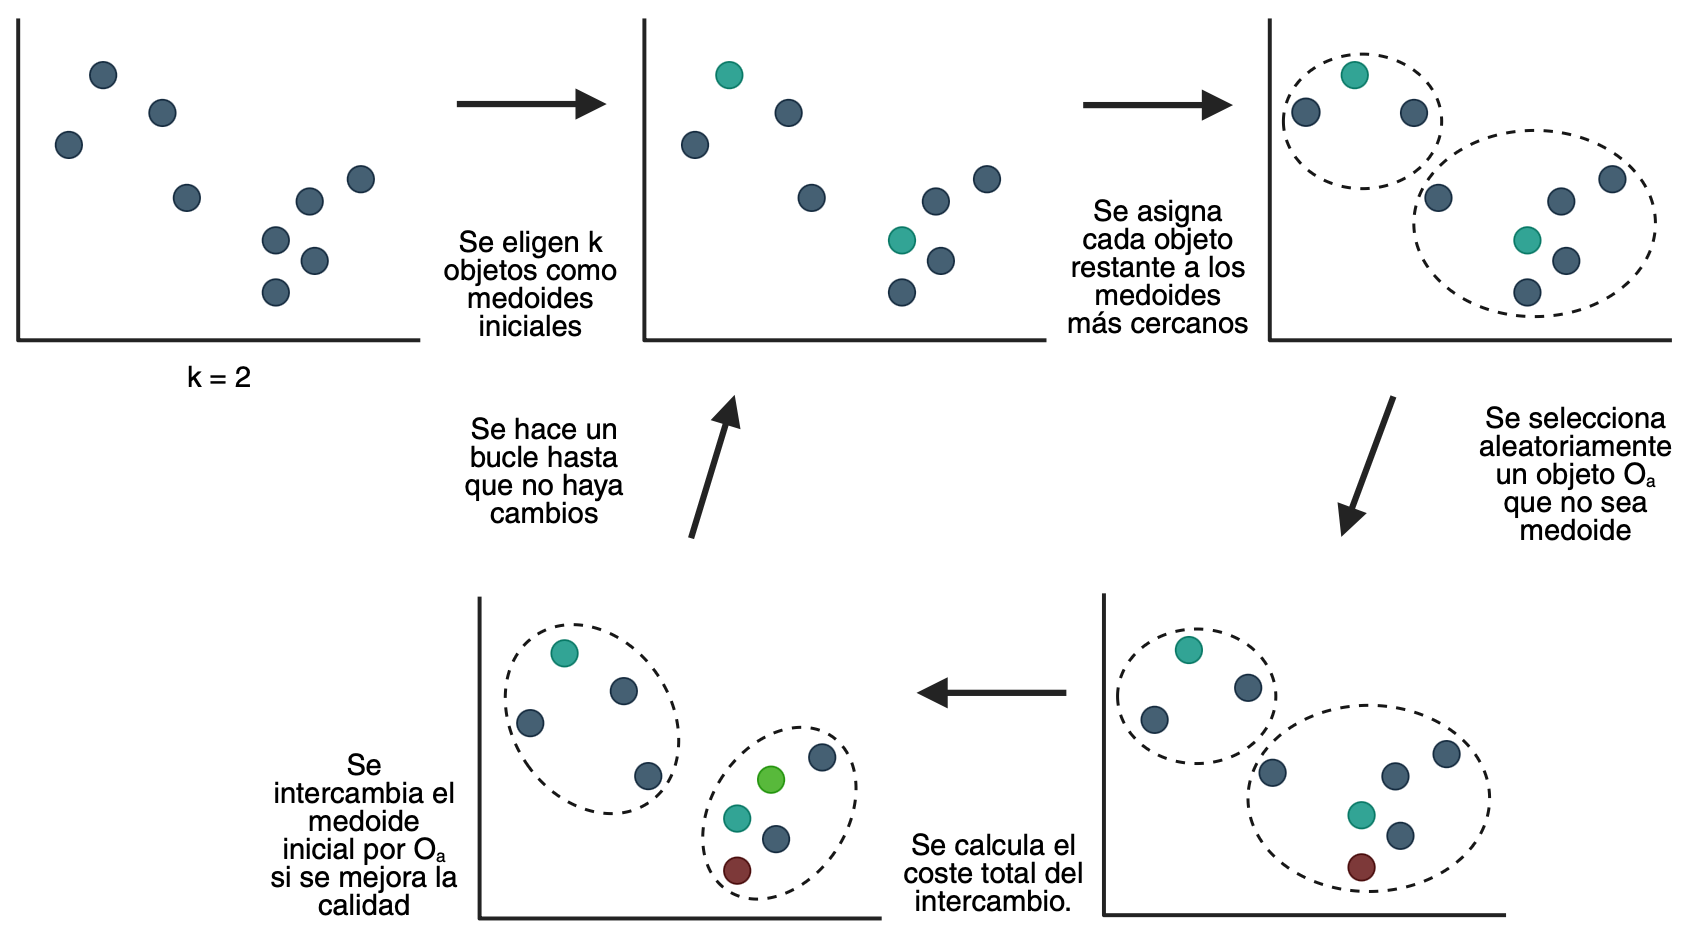
\includegraphics[width=\textwidth]{img/introduction/09_PAM.png}
    \caption[\textit{Partitioning Around Medoids}]{\textbf{Representación del algoritmo PAM.} El proceso muestra la selección aleatoria de objetos como medoides iniciales, la asignación de otros objetos a los medoides más cercanos, el cálculo del costo total y el intercambio de objetos para mejorar la calidad del \textit{clustering} hasta que no haya cambios. Imagen creada con BioRender \cite{biorender2025}.}
    \label{fig:PAM}
\end{figure}

El uso de estos algoritmos en el análisis del microbioma biomédico ha crecido significativamente. Numerosos estudios integran estas metodologías para identificar taxones relevantes en diversas patologías \cite{marcos2021applications}. Por ejemplo, en la EII, las técnicas como \textit{K-means} y HC se han utilizado para clasificar a los pacientes en subgrupos basados en la composición de su microbioma intestinal. Esto ha permitido descubrir diferencias en la abundancia de ciertos taxones, las cuales se correlacionan con la patogénesis de la EII y con la respuesta al tratamiento \cite{bakir2022inflammatory}. De manera similar, en investigaciones sobre el CCR, algoritmos como PAM han facilitado la identificación de subgrupos de pacientes con perfiles de diversidad microbiana distintos y la presencia de taxones como \textit{Fusobacterium}. Esto se ha relacionado con diferencias en la progresión tumoral y en la respuesta a tratamientos inmunoterapéuticos \cite{liu2024improved, marcos2021applications}.


\paragraph{Rendimiento y validación}

En el campo del \textit{clustering} no supervisado, la evaluación del rendimiento se centra en la calidad y coherencia de los \textit{clusters} formados. En esta sección se explican las métricas de rendimiento más comunes y las estrategias de validación que aseguran la solidez de los resultados.

\textbf{Rendimiento}

Es importante evaluar el resultado de los algoritmos de \textit{clustering}; sin embargo, es difícil definir cuándo el resultado de un \textit{clustering} es aceptable. Por esta razón, existen técnicas e índices para la evaluación de un \textit{clustering} realizado que se centran en la calidad y coherencia de los grupos formados. A continuación, se muestran algunos de los índices más utilizados \cite{halkidi2001clustering}.

\textbf{Índice de Silueta}: este índice evalúa la calidad al comparar la cohesión dentro de un \textit{cluster} (qué tan cerca está un punto de los otros en su mismo grupo) con la separación entre \textit{clusters} (qué tan lejos está de los puntos en el \textit{cluster} más cercano). Para cada punto, la silueta se define como:

\begin{equation}
    s(i) = \frac{b(i) - a(i)}{\max(a(i), b(i))} 
\end{equation}
\myequations{Índice de Silueta}
\begin{itemize}
\item Donde $a(i)$  es la distancia media entre $(i)$ y todos los otros puntos en el mismo \textit{cluster}, y $b(i)$ es la distancia media entre $(i)$ y todos los puntos del \textit{cluster} más cercano.
\end{itemize}

Los valores de este índice varían de -1 a 1, donde un valor cercano a 1 indica que los puntos están bien agrupados, un valor cercano a 0 sugiere que los \textit{clusters} se superponen, y un valor negativo indica que un punto podría estar en el grupo incorrecto.

\textbf{Índice de Davies-Bouldin}: este índice evalúa la compacidad de los \textit{clusters} y la separación entre ellos. Se calcula como el promedio de la similitud entre cada \textit{cluster} y su \textit{cluster} más similar:

\begin{equation}
    \text{DB} = \frac{1}{n} \sum_{i=1}^{n} \max_{j \neq i} \left( \frac{s_i + s_j}{d_{ij}} \right) 
\end{equation}
\myequations{Índice de Davies-Bouldin}
\begin{itemize}
\item Donde $s_i$ es la dispersión del \textit{cluster} $(i)$ (típicamente la media de distancias entre los puntos del \textit{cluster} y su centroide), y $d_{ij}$ es la distancia entre los centroides de los \textit{clusters} $(i)$ y $(j)$.
\end{itemize}

Un valor de Davies-Bouldin más bajo indica un mejor modelo de \textit{clustering}.


\textbf{Índice de Rand ajustado (ARI)}: este índice evalúa la concordancia entre dos \textit{clusters}, teniendo en cuenta el azar. Se define como:

\begin{equation}
    \text{ARI} = \frac{\text{RI} - \text{E[RI]}}{\max(\text{RI}) - \text{E[RI]}}
\end{equation}
\myequations{Índice de Rand ajustado}
\begin{itemize}
\item Donde $RI$ (índice de Rand) es la proporción de pares de puntos que están consistentemente en el mismo o diferente \textit{cluster} en ambas agrupaciones, y $E[RI]$ es el valor esperado de $RI$ bajo una distribución aleatoria.
\end{itemize}
El ARI tiene un valor máximo de 1, que indica agrupaciones idénticas, y puede ser negativo si el rendimiento es peor que el esperado por azar.

Estas medidas ofrecen diferentes perspectivas sobre la calidad de un \textit{clustering} y ayudan a seleccionar el modelo más adecuado según los objetivos y características del conjunto de datos. En el caso de la presente Tesis Doctoral, al realizar el \textit{clustering} en el tercer trabajo \cite{paper3}, se utilizó el paquete NbClust \cite{charrad2014nbclust} (que cuenta con más de 20 índices de evaluación) para calcular los índices de rendimiento de los \textit{clusters} obtenidos.

\textbf{Validación}

Para asegurar la robustez del \textit{clustering}, se emplean estrategias de validación. Para este propósito, se utilizó ConsensusClusterPlus (CCP) \cite{wilkerson2010consensusclusterplus}. Una de las características distintivas de CCP es su estrategia de submuestreo repetido. Este remuestreo se realiza sin reemplazo, generando subconjuntos que pueden representar aproximadamente el 50–80 \% de los datos originales, y se ejecuta de forma reiterada (normalmente con un número de repeticiones que suele ser 100 o más) para capturar la variabilidad inherente en la estructura de los datos. Cada subconjunto obtenido se utiliza para ejecutar un algoritmo base de \textit{clustering}, lo que genera una partición o asignación provisional de \textit{clusters} que servirá en el posterior cálculo del consenso.

Una vez generadas las particiones a partir de diversas repeticiones, se procede a evaluar la estabilidad y robustez de los agrupamientos. Para ello, se calcula una matriz de consenso, en la cual cada elemento (\textit{i}, \textit{j}) representa la proporción de veces que las muestras \textit{i} y \textit{j} fueron asignadas al mismo \textit{cluster} a lo largo de todas las iteraciones. Dicho valor, que varía entre 0 y 1, indica la fortaleza de la asociación entre cada par de muestras; valores cercanos a 1 sugieren que las muestras presentan un agrupamiento robusto, mientras que valores intermedios indican asignaciones ambiguas. Además, se calculan métricas adicionales que permiten cuantificar la estabilidad interna de cada \textit{cluster}, como el \textit{item-consensus} (que mide la representatividad de una muestra dentro de su \textit{cluster} asignado) o el \textit{cluster-consensus}, que resume la estabilidad global de cada \textit{cluster}. Esta evaluación estadística proporciona una base cuantitativa para determinar la robustez del \textit{clustering}, permitiendo además la comparabilidad de resultados entre diferentes configuraciones y parámetros.

En resumen, el aprendizaje no supervisado resulta especialmente valioso porque parte directamente de los propios datos del microbioma, sin imponer etiquetas clínicas ni supuestos previos, para desentrañar la variabilidad que la información clínica no alcanza a explicar. Al estratificar primero las muestras exclusivamente según sus perfiles microbianos, emergen subgrupos biológicos latentes que después pueden asociarse retrospectivamente con fenotipos clínicos (como severidad, evolución o respuesta terapéutica), en lugar de forzar dichas categorías de antemano. Esta estrategia, apoyada con medidas de rendimiento y validación robustas, permite extraer información sin restricciones impuestas por las etiquetas, revelar patrones no evidentes y priorizar candidatos a biomarcadores microbianos que orienten una estratificación más precisa y, potencialmente, diagnósticos y decisiones terapéuticas más personalizadas.

\begin{figure}[!h]
    \centering
    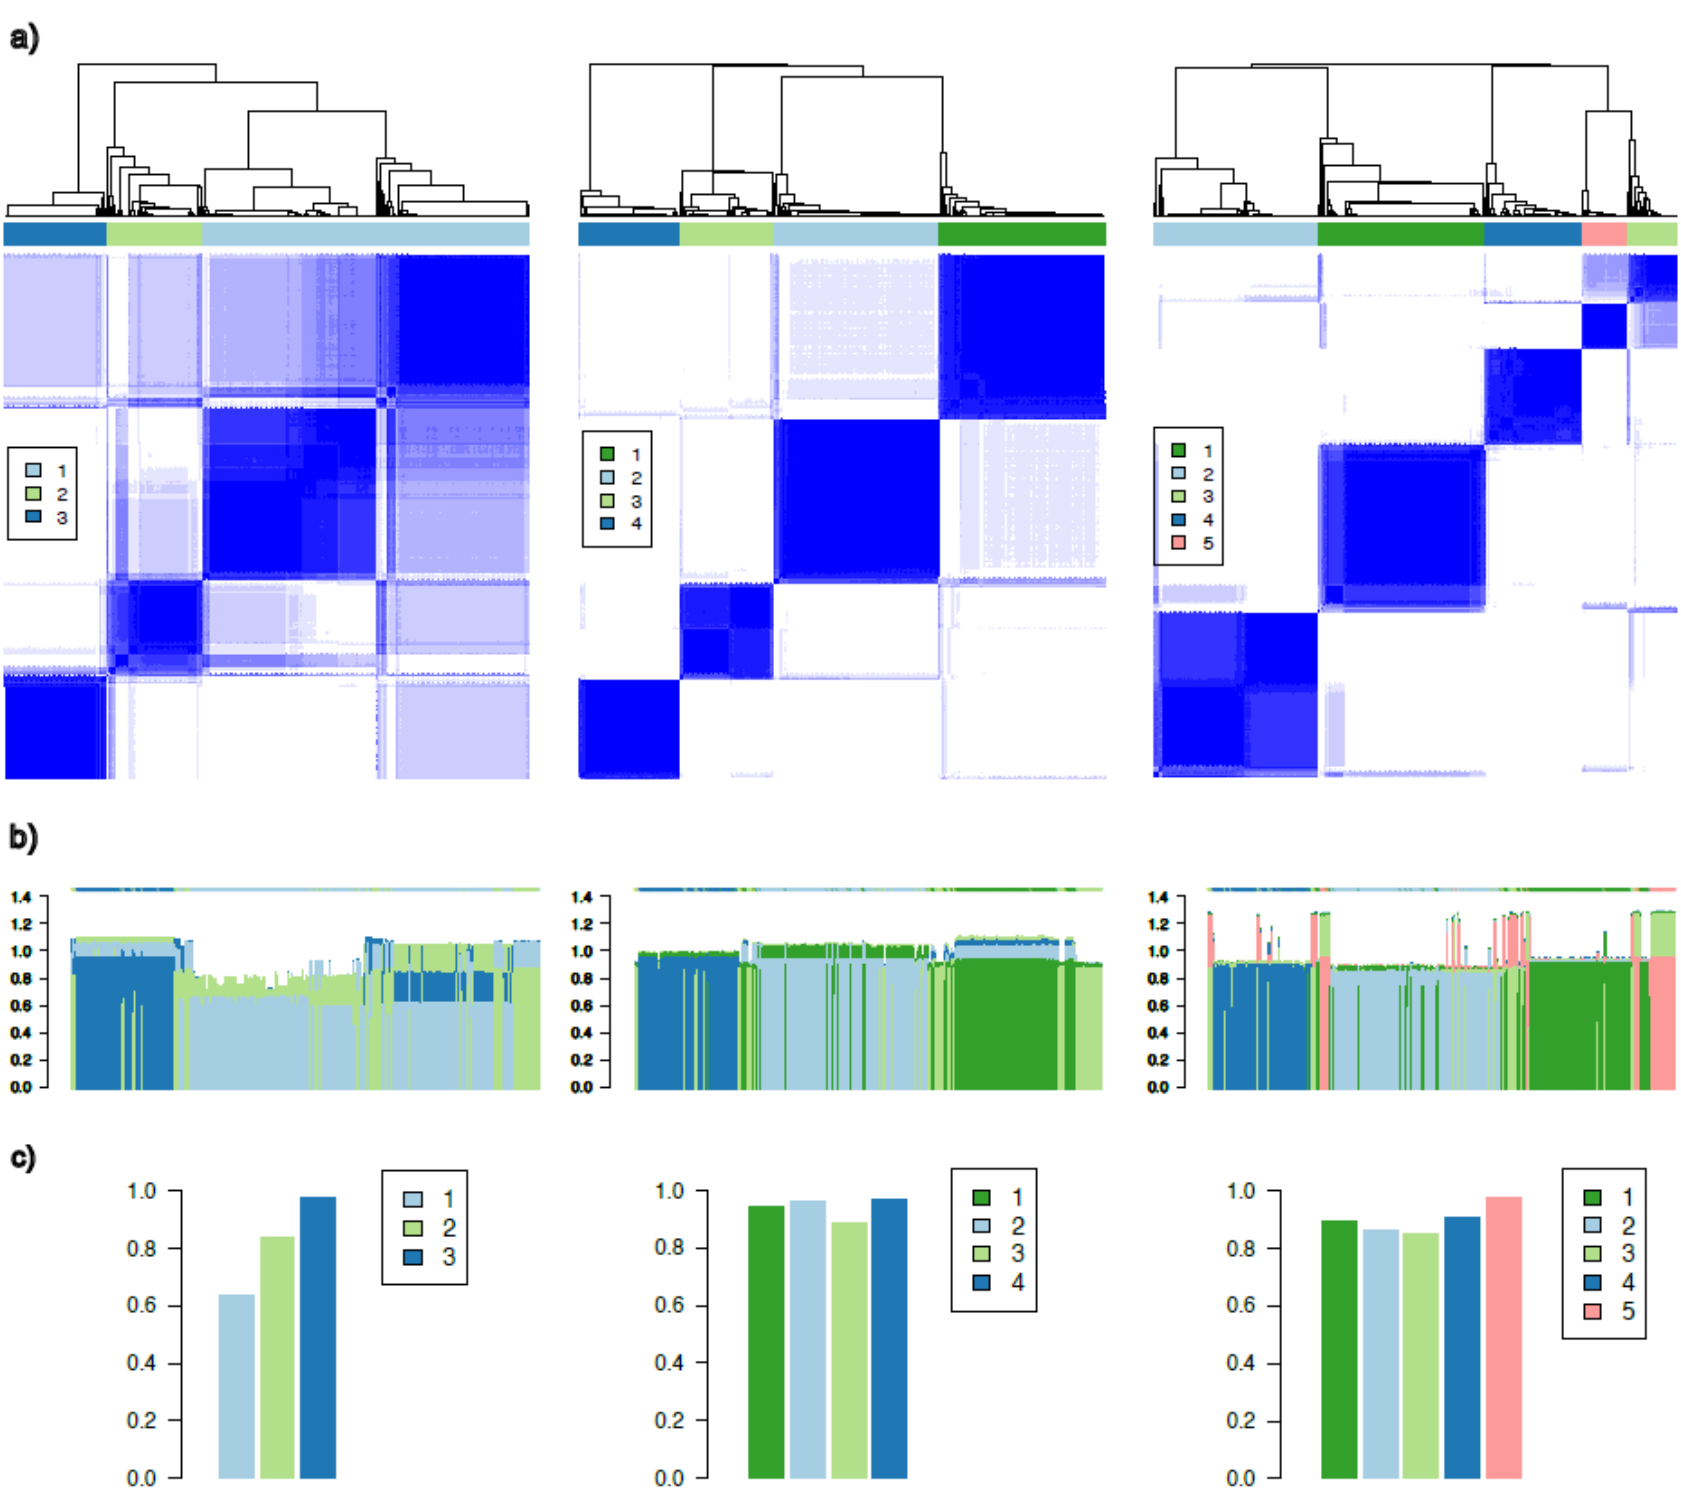
\includegraphics[width=\textwidth]{img/introduction/CCPV.png}
    \caption[ConsensusClusterPlus]{\textbf{Representación gráfica de las métricas de CCP.} a) \textit{Matrix-consensus}: matrices donde las muestras se organizan en filas y columnas. La intensidad muestra la probabilidad de agrupamiento, donde el blanco es 0 y el azul oscuro es 1. b) \textit{Item-consensus}: muestra el consenso de la asignación de cada muestra a un grupo concreto para un número determinado de grupos k. Cuanto más alta es la barra de un grupo concreto, mayor es el consenso de que la muestra pertenece a ese grupo. c) \textit{Cluster-consensus}: muestra el valor de consenso de los grupos en cada k. Los valores altos indican que un grupo tiene una alta estabilidad y los valores bajos indican que un grupo tiene una baja estabilidad.}
    \label{fig:CCP}
\end{figure}


\subsubsection{Aprendizaje supervisado}

El aprendizaje supervisado es un tipo de ML donde los modelos se entrenan con datos que ya tienen etiquetas de salida. El objetivo es que el modelo aprenda la relación entre las variables de entrada (características) y las de salida (etiquetas) para poder predecir resultados en nuevos datos. Este tipo de aprendizaje se divide en dos categorías principales: clasificación, que predice una categoría o etiqueta discreta, y regresión, que predice un valor continuo. \cite{bishop2006pattern}.

El aprendizaje supervisado es particularmente útil para abordar la complejidad y la alta dimensionalidad de los datos del microbioma, ya que permite construir modelos predictivos que identifican patrones microbianos asociados con estados patológicos específicos. En este contexto, se emplea este tipo de aprendizaje bajo la asunción explícita de que el uso de modelos interpretables entrenados con datos del microbioma no solo permite predecir un estado clínico, sino también inspeccionar los modelos para identificar los taxones con mayor peso en la decisión. Esta lectura de la importancia permite vincular los taxones destacados con funciones y rutas potencialmente implicadas, generar hipótesis contrastables y priorizar validaciones en cohortes externas.

A continuación se presentan los diferentes tipos de modelos de aprendizaje supervisado utilizados en esta Tesis Doctoral.

\paragraph{Modelos lineales}

Los modelos lineales son algunos de los algoritmos de aprendizaje supervisado más simples e interpretables. Asumen una relación lineal entre las características de entrada y la salida, lo que les permite estimar la variable objetivo mediante una suma ponderada de los predictores. La ecuación se define como:

\begin{equation}
Y = \beta_0 + \beta_1 X_1 + \beta_2 X_2 + \ldots + \beta_n X_n + \epsilon
\end{equation}
\myequations{Regresión lineal}
\begin{itemize}
\item Donde $Y$ es la variable objetivo que queremos predecir. $\beta_0$ es la intersección (o término independiente) del modelo. $\beta_1$, $\beta_2$, ..., $\beta_n$ son los coeficientes que representan el peso de cada predictor. $X_1$, $X_2$, ..., $X_n$ son las características de entrada. Y $\epsilon$ es el término de error, que captura la variabilidad no explicada por el modelo.
\end{itemize}

Este modelo reporta un valor continuo, es decir, estaríamos hablando de un problema de regresión. Mientras que, para problemas de clasificación, es necesario acotar este rango de respuesta entre 0 y 1. En lugar de modelar $Y$ directamente, se modela la probabilidad de que una observación pertenezca a una clase específica, convirtiendo el modelo en una regresión logística \cite{hosmer2013applied}. Se establece un umbral para la clasificación de las observaciones. Es decir, suponiendo una clasificación binaria, con el umbral definido en 0,5, las predicciones menores a 0,5 serán categorizadas en una clase, mientras que las mayores a 0,5 pertenecerán a la otra. Esta ecuación se define como:

\begin{equation}
P(Y=1 | X) = \sigma(\beta_0 + \beta_1 X_1 + \beta_2 X_2 + \ldots + \beta_n X_n)
\end{equation}
\myequations{Regresión logística}
\begin{itemize}
\item Donde $\sigma(z)= \frac{1}{1 + e^{-z}}$ es la función sigmoide que mapea cualquier valor de (z) a un rango entre 0 y 1. En este contexto:
\begin{itemize}
\item Si $P(Y=1 | X) > 0.5$ se clasifica como la clase 1.
\item Si $P(Y=1 | X) \leq 0.5$ se clasifica como la clase 0.
\end{itemize}
\end{itemize}

No obstante, cuando los datos presentan multicolinealidad o un alto número de variables, los modelos lineales simples pueden sufrir de sobreajuste, perdiendo su capacidad para generalizar. Para mitigar esto, se utilizan modelos lineales regularizados, como los ajustados por el algoritmo \textit{glmnet}. Este algoritmo aplica penalizaciones (\textit{LASSO} y \textit{Ridge}) a los coeficientes para simplificar el modelo y mejorar su rendimiento \cite{friedman2010regularization}.

\textit{LASSO} realiza la regularización mediante la penalización de la suma de los valores absolutos de los coeficientes $\beta$ (norma $l_1$). Esto tiende a reducir algunos de estos coeficientes a cero, permitiendo eliminar características irrelevantes y realizar una selección de características efectiva. Esto es especialmente útil en conjuntos de datos de alta dimensión.

\textit{Ridge} aplica penalización a la suma de los cuadrados de los coeficientes (norma $l_2$). No lleva estos coeficientes exactamente a cero, sino que reduce su magnitud para limitar el efecto de colinealidad entre variables. Su principal fortaleza está en la estabilización de los coeficientes en presencia de multicolinealidad.

La función objetivo de \textit{glmnet} para regresión logística combina la discrepancia de las predicciones con una penalización llamada \textit{Elastic Net}, que es una mezcla de las regularizaciones $l_1$ y  $l_2$:

\begin{equation}
\min_{(\beta_0, \beta) \in \mathbb{R}^{p+1}} - \left[ \frac{1}{N} \sum_{i=1}^{N} y_i \cdot (\beta_0 + x_i^T \beta) - \log(1 + e^{(\beta_0 + x_i^T \beta)}) \right] + \lambda \left[ (1 - \alpha) \frac{\|\beta\|_2^2}{2} + \alpha \|\beta\|_1 \right]
\end{equation}
\myequations{Función objetivo de \textit{glmnet}}
\begin{itemize}
\item Donde el primer elemento es el \textit{Log-likelihood} de la regresión logística: mide la discrepancia entre las predicciones y las etiquetas reales. El segundo elemento es la penalización \textit{Elastic Net}: combinación de las regularizaciones $l_1$ y $l_2$.

\item Donde $\lambda$ es un parámetro que controla la intensidad de la penalización en ambos métodos. Valores grandes de $\lambda$ limitan la magnitud de los coeficientes, simplificando el modelo, mientras que valores pequeños permiten más complejidad. Y $\alpha$ es el parámetro que regula el tipo de penalización (o mezcla de ambas):
\begin{itemize}
\item $\alpha$ = 1 equivale a \textit{LASSO}, ejerciendo penalización $l_1$ sobre los parámetros.
\item $\alpha$ = 0 equivale a \textit{Ridge}, ejerciendo penalización $l_2$ sobre los parámetros.
\end{itemize}
\end{itemize}

En los modelos lineales regularizados, los coeficientes ajustados proporcionan una interpretación valiosa sobre la importancia de cada variable en el modelo. Esto es especialmente útil en datos del microbioma, donde se pueden analizar los coeficientes para identificar qué taxones tienen más peso en las predicciones. Al observar cuáles son los coeficientes más grandes, es posible inferir qué taxones son más relevantes en el problema estudiado.

\paragraph{Modelos basados en \textit{kernels}}

Los modelos basados en \textit{kernels}, como las \textit{Support Vector Machines} (SVM), extienden los clasificadores lineales para manejar datos no separables linealmente. Su idea central es mapear los datos originales a un espacio de mayor dimensión donde la separación lineal es más factible. Esto se logra mediante una función \textit{kernel} que realiza la transformación de forma implícita \cite{cortes1995support}.

Como se representa en la Figura \ref{fig:SVM}, las SVM buscan maximizar el margen entre clases mediante un hiperplano definido por un número de vectores soporte (subconjunto de puntos de datos que son cruciales para definir el límite de decisión entre diferentes clases). Un hiperplano es un subespacio de dimensiones (n-1) que divide el espacio de características en regiones distintas, cada una correspondiente a una clase. En un problema de dos dimensiones, el hiperplano es una línea; en tres dimensiones, es un plano; y en dimensiones superiores, se extiende a un espacio que divide los grupos de datos.

\begin{figure}[h]
    \centering
    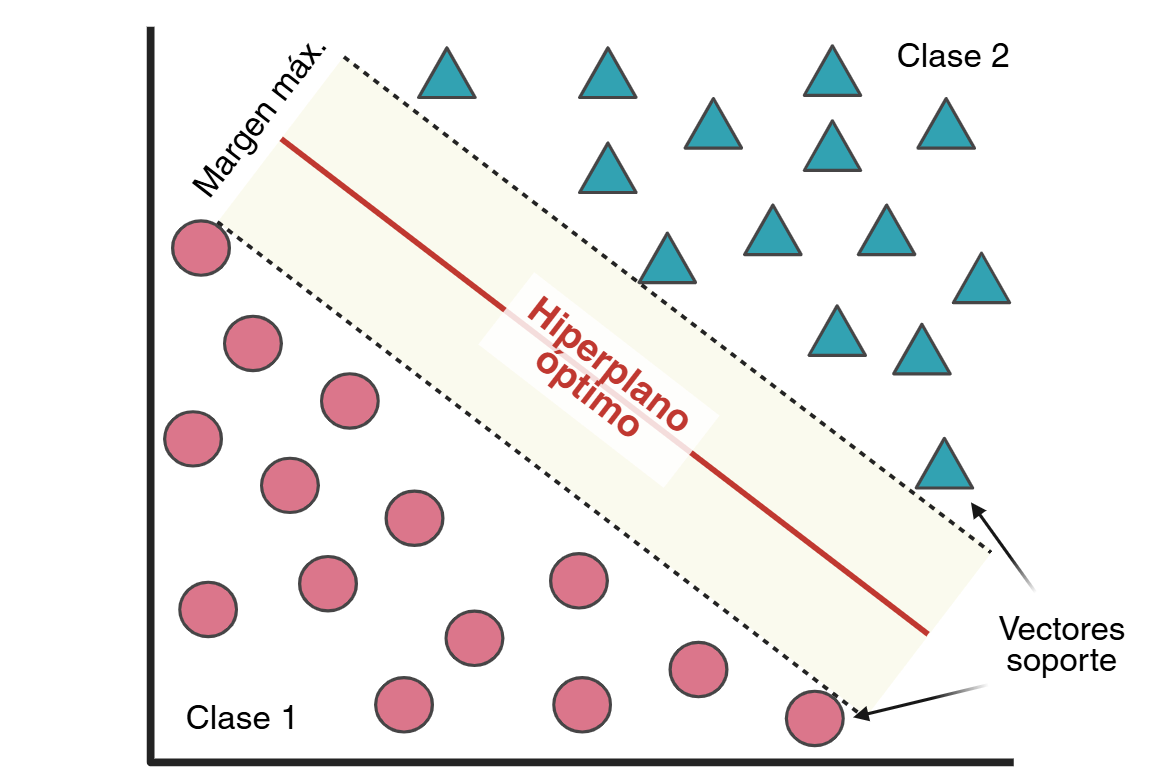
\includegraphics[width=0.65\textwidth]{img/introduction/09_SVM.png}
    \caption[Representación de \textit{Support Vector Machines}]{\textbf{Ilustración de un modelo SVM en un problema de dos dimensiones.} La imagen muestra el hiperplano óptimo que separa dos clases con el margen máximo, utilizando vectores de soporte que determinan la posición y orientación del hiperplano para lograr la máxima separación entre las clases. Imagen creada con BioRender \cite{biorender2025}.}
    \label{fig:SVM}
\end{figure}


En problemas donde las clases sean linealmente separables, van a existir infinitos hiperplanos que separen dichas clases; aquí es donde entran los métodos de optimización. En esta situación, el objetivo es buscar el hiperplano que consiga el mayor margen entre clases, es decir, maximizar la distancia mínima entre el hiperplano y las observaciones.

En situaciones donde los datos no son linealmente separables, las SVM utilizan dos enfoques clave para abordar el problema. Primero, se puede optar por el enfoque \textit{soft margin}; esto es, permitir que algunas instancias de datos queden del lado incorrecto del margen (muestras de una clase queden del lado contrario del hiperplano). Este enfoque introduce variables de holgura que permiten errores de clasificación controlados, logrando un balance entre maximizar el margen y minimizar el error, regulado por un parámetro (C). Otro enfoque es el denominado \textit{Kernel Trick}, que se basa en transformar los datos a un espacio de mayor dimensión donde un hiperplano puede separarlos linealmente. Esto se realiza mediante funciones \textit{kernel} polinómicas, \textit{Radial Basis Function} (RBF) o sigmoides, entre otras. Estas funciones calculan estas transformaciones de forma implícita. Este enfoque permite que las SVM encuentren fronteras de decisión no lineales, haciendo posible separar eficazmente las clases en el espacio transformado (Figura \ref{fig:SVM_kernels}) \cite{scholkopf2002learning}.


\begin{figure}[h]
    \centering
    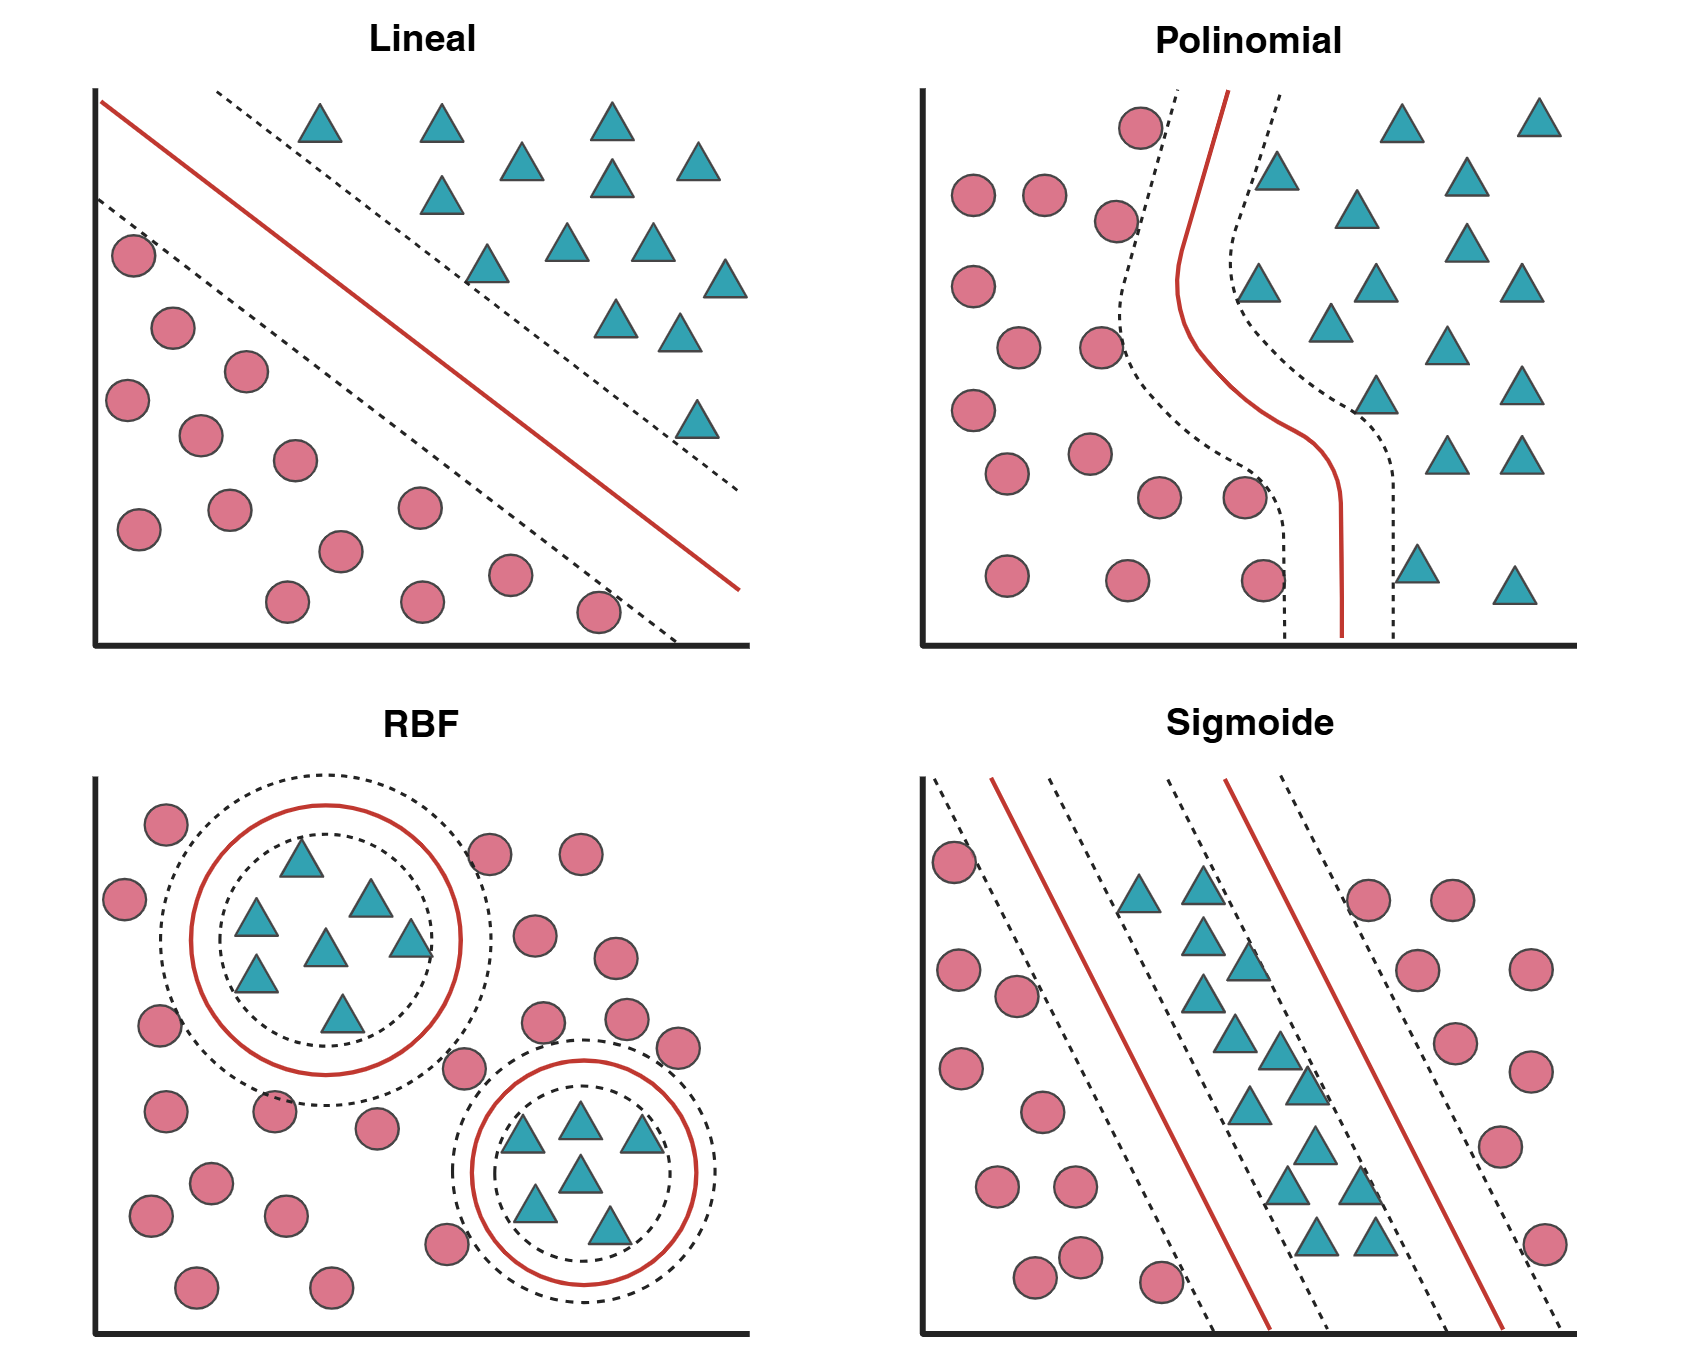
\includegraphics[width=0.8\textwidth]{img/introduction/10_Kernels.png}
    \caption[Tipos de \textit{Kernels} de SVM]{\textbf{Ejemplos de funciones \textit{kernel} utilizadas en SVMs: lineal, polinomial, RBF y sigmoide.} Estas enfoques permiten transformar los datos a distintas dimensiones, posibilitando la separación de clases a través de fronteras de decisión tanto lineales como no lineales. Imagen creada con BioRender \cite{biorender2025}.}
    \label{fig:SVM_kernels}
\end{figure}

Los hiperparámetros más importantes en este tipo de modelo son el parámetro de penalización C, que controla el equilibrio entre maximizar el margen y minimizar el error de clasificación, la elección del \textit{kernel} y los parámetros específicos del \textit{kernel}, como el grado en el \textit{kernel} polinómico o $\gamma$ en el \textit{kernel} RBF. Los ajustes a estos hiperparámetros pueden afectar significativamente tanto la capacidad de generalización como la eficiencia computacional del modelo. En el ámbito de la investigación del microbioma, los modelos basados en kernels ofrecen una herramienta poderosa para capturar relaciones complejas y no lineales entre las características microbianas y los resultados clínicos.

\paragraph{Modelos basados en árboles}

Estos modelos construyen una estructura similar a un árbol a partir de reglas lógicas. Estas reglas dividen las observaciones del conjunto de entrenamiento basándose en sus variables, lo que permite predecir el valor de la variable de salida.

Dentro de este tipo de modelos, el algoritmo más simple es el árbol de decisión (Figura \ref{fig:DT}). Este algoritmo se compone de un nodo raíz, nodos internos (o nodos de decisión) y nodos hoja (o nodos terminales), unidos por ramas. El nodo raíz es el punto de partida del árbol, donde se encuentra la primera decisión o la característica más importante para la clasificación o predicción. Los nodos internos representan decisiones intermedias o divisiones basadas en las características de los datos, conectando el nodo raíz con los nodos hoja. Los nodos hoja son los nodos finales del árbol, que representan los resultados o predicciones finales del modelo. Las ramas son las líneas que conectan los nodos, mostrando los diferentes caminos o resultados posibles de cada decisión \cite{quinlan1986induction}.


\begin{figure}[h]
    \centering
    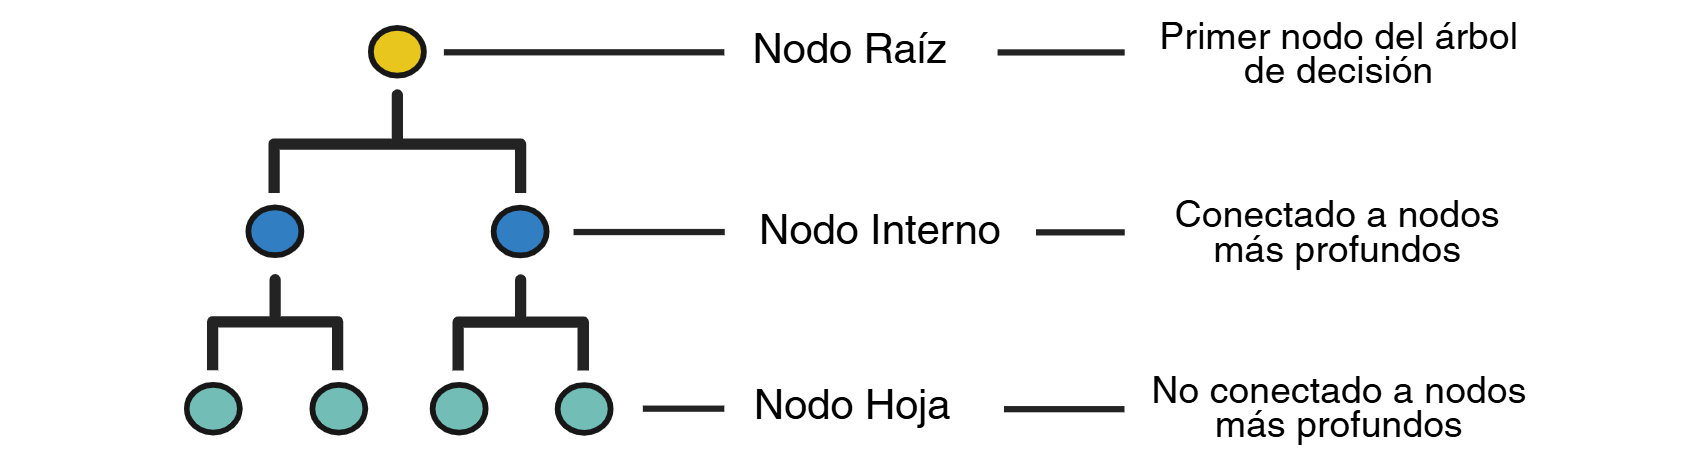
\includegraphics[width=0.95\textwidth]{img/introduction/11_DT.png}
    \caption[Representación de un árbol de decisión]{\textbf{Diagrama de un árbol de decisión mostrando la estructura básica: nodo raíz, nodo interno y nodo hoja.} El nodo raíz inicia el árbol, los nodos internos están conectados a nodos más profundos y los nodos hoja representan las decisiones finales sin conexiones adicionales. Imagen creada con BioRender \cite{biorender2025}.}
    \label{fig:DT}
\end{figure}

Las principales ventajas de este tipo de algoritmo son que son fácilmente interpretables, manejan tanto datos categóricos como continuos, presentan robustez a \textit{outliers} y son relativamente rápidos de entrenar. Sin embargo, en muchos casos, la predicción de un solo árbol no es suficiente (logrando rendimientos bajos) y tienden a sobreajustarse a los datos de entrenamiento.

Para contrarrestar esta debilidad, se han desarrollado métodos de \textit{ensemble learning}, como los \textit{Random Forest} (RF) y los \textit{eXtreme Gradient Boosting} (XGBoost).

La base de RF es emplear muchos árboles de decisión para buscar la mejor solución a un problema complejo, basándose en la premisa de que, al aumentar el número de árboles, se incrementa la precisión del resultado (Figura \ref{fig:RF}). Este algoritmo se basa en un método de submuestreo llamado \textit{Bootstrap Aggregating}. Es decir, se generan varios conjuntos de datos de entrenamiento a partir del conjunto original, utilizando muestreo con reemplazo. Para cada conjunto de datos generado, se entrena un árbol de decisión independiente. Además, en cada nodo de cada árbol, se selecciona aleatoriamente un subconjunto de características. La mejor división se elige solo del subconjunto seleccionado, lo que introduce diversidad entre los árboles. Al realizar las predicciones, en problemas de clasificación se lleva a cabo un voto mayoritario entre las predicciones de los árboles, mientras que en regresión se calcula la media de las predicciones de todos los árboles \cite{breiman2001random}.

\begin{figure}[h]
    \centering
    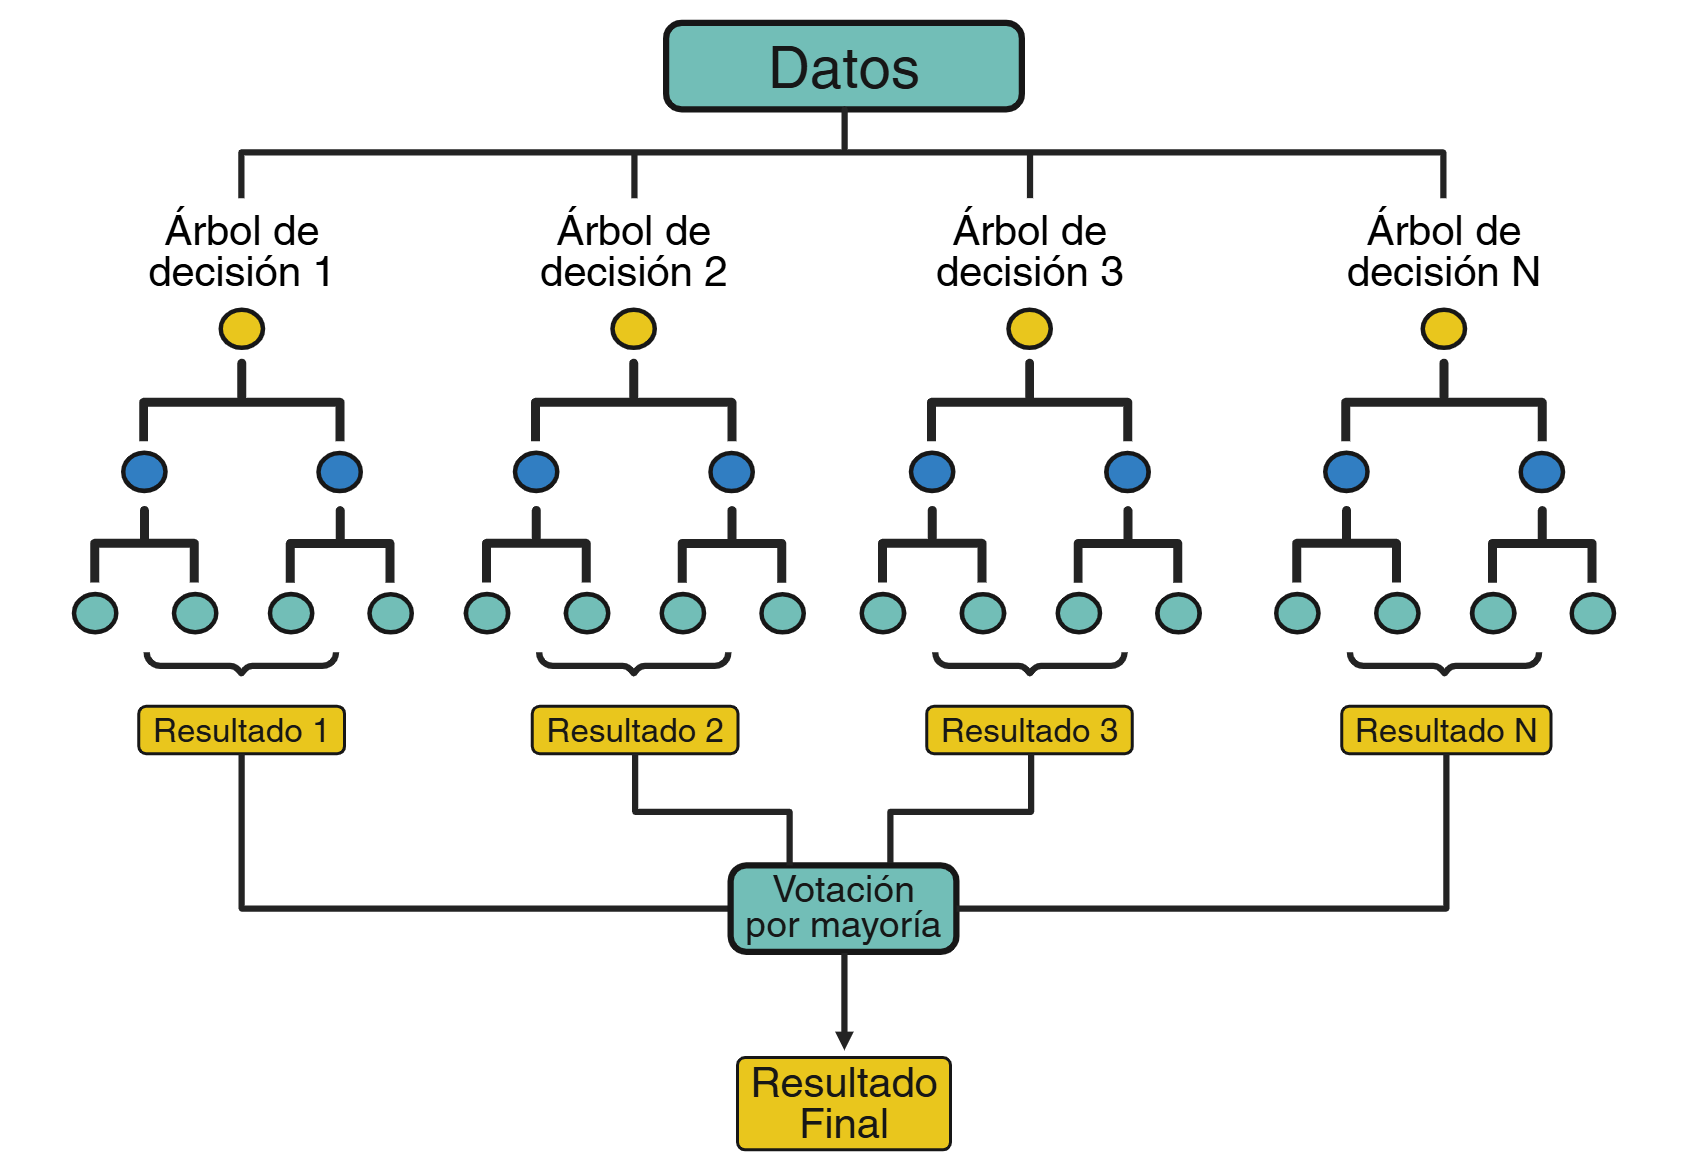
\includegraphics[width=\textwidth]{img/introduction/12_RF.png}
    \caption[Representación de \textit{Random Forest}]{\textbf{Representación de un RF.} Se muestran múltiples árboles que generan resultados individuales a partir de los datos. El resultado final se determina mediante votación por mayoría, combinando la decisión de cada árbol para mejorar la precisión del modelo. Imagen creada con BioRender \cite{biorender2025}.}
    \label{fig:RF}
\end{figure}


Los hiperparámetros críticos para los modelos basados en RF incluyen el número de variables escogidas en cada división del árbol, el tamaño mínimo de un nodo terminal, la profundidad máxima de cada árbol y el número de árboles utilizados para construir el RF. Respecto al número de variables que se consideran en cada división del árbol, en clasificación, una opción común es usar la raíz cuadrada del número total de variables, mientras que en regresión, se suele utilizar un tercio del total de variables. El tamaño mínimo de un nodo terminal controla el tamaño de los nodos al final de los árboles; un valor menor permite modelos más complejos, ya que los árboles tendrán más profundidad. La profundidad máxima de cada árbol en el bosque hace referencia al número máximo de niveles o capas que puede tener un árbol individual desde la raíz hasta los nodos terminales. Limitar la profundidad puede ayudar a prevenir el sobreajuste, pero un valor muy bajo puede resultar en un modelo demasiado simple. Finalmente, respecto al número de árboles, generalmente, cuantos más árboles, mejor será la estabilización del modelo y su capacidad para generalizar.

En cuanto a la interpretabilidad de los modelos creados con RF, destaca la posibilidad de calcular la importancia de cada variable. La manera más sencilla es contabilizar la cantidad de veces que cada variable es seleccionada a lo largo de todos los árboles que conforman el RF. Otra medida utilizada es la \textit{Gini importance} (o disminución media de la impureza). Como ya se ha comentado, cada árbol de decisión está conformado por un conjunto de nodos internos y hojas. En el nodo interno, la característica seleccionada se utiliza para tomar decisiones sobre cómo dividir el conjunto de datos en dos subconjuntos separados que presentan similitudes en sus respuestas. Se puede medir cómo cada característica disminuye la impureza de la división (la característica con la mayor disminución es seleccionada para el nodo interno), es decir, cuán homogéneos son los grupos después de la división. Para cada característica, se puede recopilar el promedio de cómo disminuye la impureza. El promedio sobre todos los árboles del bosque constituye la medida de la importancia de la característica \cite{breiman2001random}.

XGBoost, en cambio, se basa en el principio de \textit{boosting}, es decir, ajusta secuencialmente una serie de árboles de decisión donde cada árbol subsecuente corrige los errores del anterior (Figura \ref{fig:XGB}). El proceso inicia con un modelo básico que realiza predicciones. Después de evaluar estas predicciones, se observan los errores o residuos, que son las diferencias entre los valores reales y las predicciones. Estos residuos se convierten en el enfoque para el siguiente modelo. Es como si se pidiera al próximo árbol que se concentrara específicamente en las partes donde el anterior falló. Esto continúa iterativamente, con cada nuevo árbol tratando de reducir estos errores, sumando su predicción a las correcciones necesarias. Cada árbol aporta pequeñas mejoras, y al final, se combinan todas estas pequeñas mejoras para hacer predicciones mucho más precisas \cite{chen2016xgboost}.


\begin{figure}[h]
    \centering
    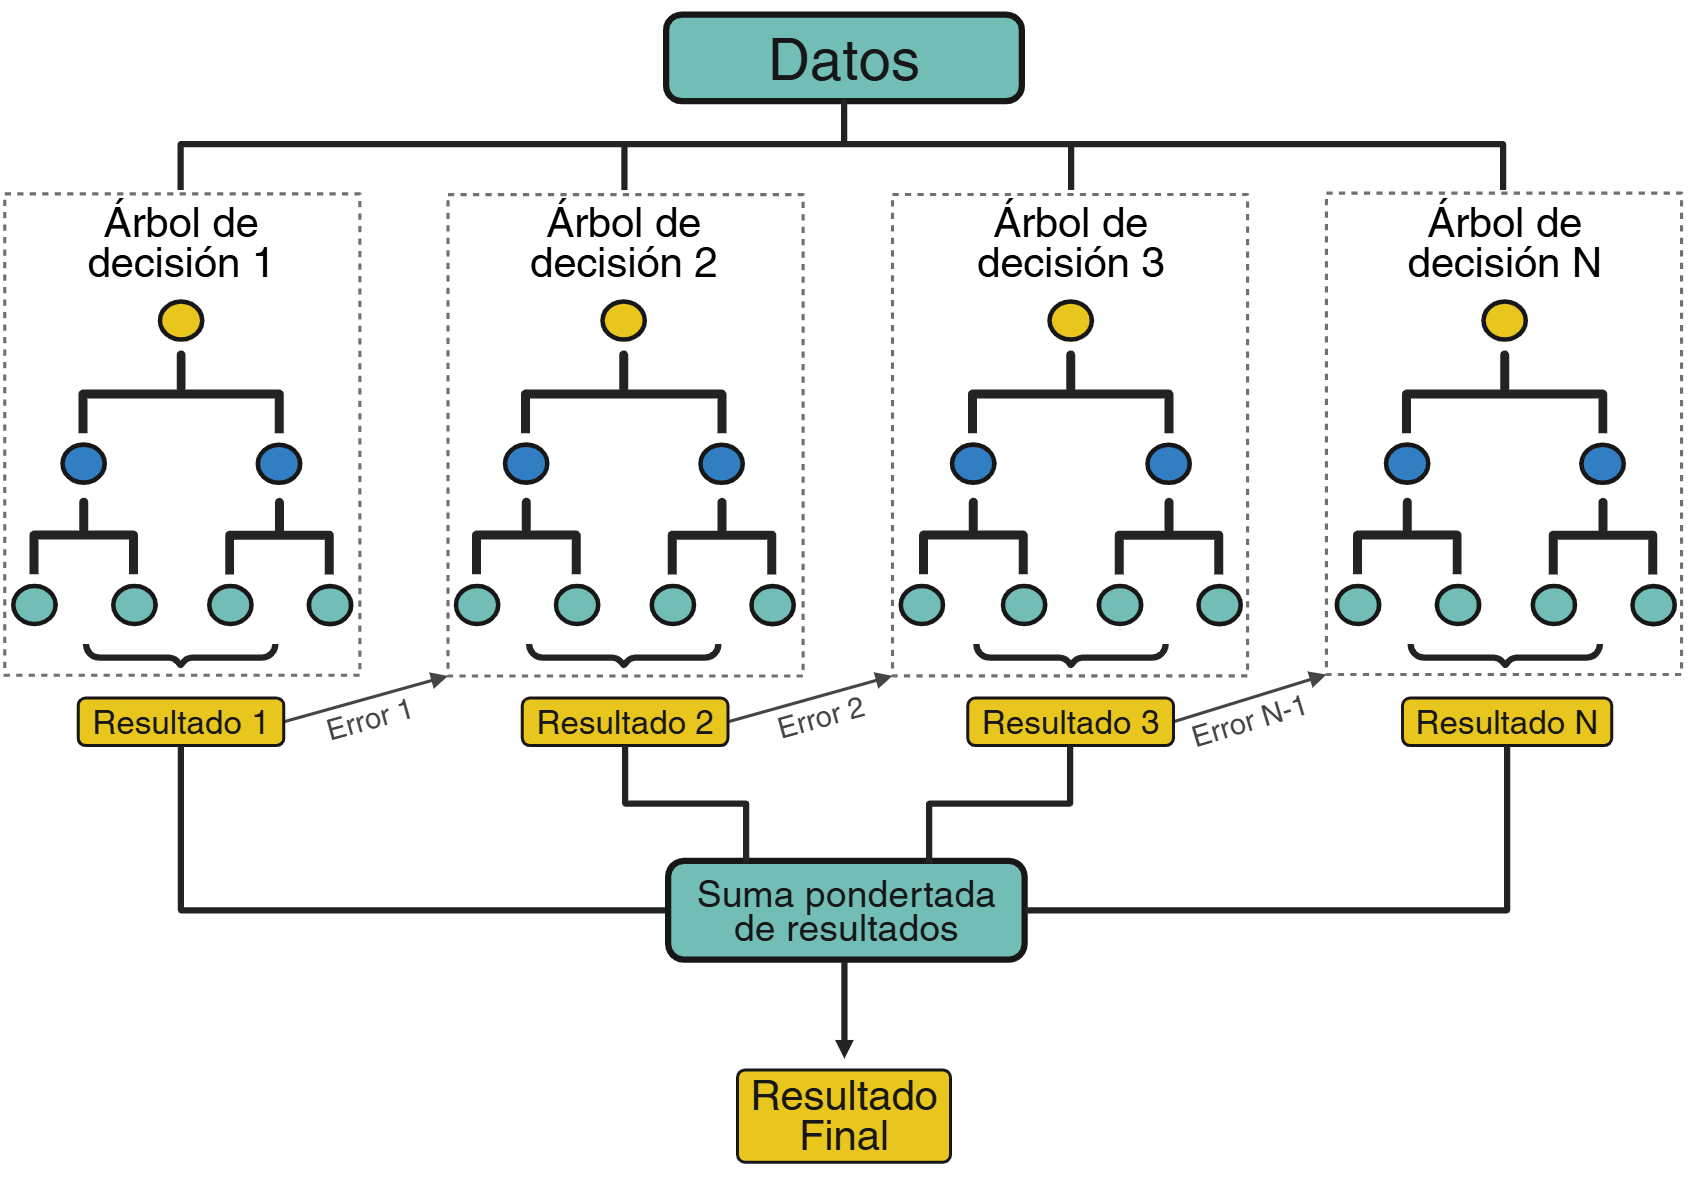
\includegraphics[width=\textwidth]{img/introduction/13_XGBOOST.png}
    \caption[Representación de \textit{eXtreme Gradient Boosting}]{\textbf{Diagrama de un modelo XGBoost.} En el se muestran cómo los árboles de decisión se construyen secuencialmente para corregir errores previos. Los resultados se combinan mediante una suma ponderada, mejorando la precisión del modelo final. Imagen creada con BioRender \cite{biorender2025}.}
    \label{fig:XGB}
\end{figure}


Los hiperparámetros críticos para este tipo de modelos incluyen aquellos tratados en RF y, además, la tasa de aprendizaje (que determina la contribución de cada árbol). Al igual que con RF, ajustar los hiperparámetros es fundamental para equilibrar la complejidad del modelo y el rendimiento de generalización, especialmente en la predicción de biomarcadores del microbioma, donde las relaciones subyacentes pueden ser no lineales y complejas.

XGBoost, al igual que RF, permite evaluar la importancia de las variables mediante métricas como la ganancia, la cobertura y la frecuencia. La ganancia mide la mejora en la función objetivo al dividir los datos con una característica, donde un valor alto indica su relevancia para la predicción. En contraste, la cobertura representa la proporción de observaciones afectadas por dicha característica, sugiriendo una mayor capacidad de generalización. Por último, la frecuencia contabiliza cuántas veces se utiliza una característica para dividir nodos, sin evaluar la calidad de su contribución. Estas métricas en conjunto ofrecen una visión integral de la relevancia de las variables dentro del modelo \cite{chen2016xgboost}.

El uso de estos algoritmos en el ámbito del microbioma biomédico ha crecido notablemente. Diversos estudios han demostrado su efectividad para identificar firmas microbianas en diferentes enfermedades. Por ejemplo, se han usado RF y SVM para encontrar patrones microbianos asociados a la susceptibilidad a infecciones respiratorias y para discriminar entre pacientes con CCR y sujetos sanos \cite{marcos2021applications, freitas2023machine, abbasi2024machine}. En el caso de las enfermedades autoinmunes y metabólicas, la combinación de modelos lineales y no lineales permite capturar tanto relaciones directas como interacciones complejas, lo que es crucial para entender el papel del microbioma en la salud humana \cite{marcos2021applications, abbasi2024machine}.

\paragraph{Rendimiento y validación}

En el ámbito del ML, evaluar el rendimiento de un modelo de clasificación es esencial para garantizar su eficacia y capacidad de generalización. Esta sección describe las métricas de evaluación y las estrategias de validación empleadas en esta Tesis Doctoral para asegurar la robustez de los modelos.

\textbf{Rendimiento}

La salida o resultado de un modelo de clasificación se refiere a la etiqueta o categoría que el modelo asigna a cada instancia de datos en función de las características previamente aprendidas durante el entrenamiento. En el caso de la clasificación binaria, el modelo determina a cuál de dos clases pertenece una instancia específica. Sin embargo, errores en esta clasificación pueden ocurrir, lo que significa que una instancia puede ser asignada incorrectamente a una clase. Estos errores implican que no se está capturando adecuadamente la realidad de los datos, lo cual es esencial para cualquier aplicación práctica del modelo.

La matriz de confusión (Figura \ref{fig:CM}) es la base para evaluar un modelo de clasificación. Esta tabla resume el rendimiento al comparar las predicciones con las etiquetas reales. Sus cuatro componentes principales son:

\begin{itemize}
\item Verdaderos Positivos (VP): el modelo predice correctamente la clase positiva. Por ejemplo, si el modelo se utiliza para diagnosticar una enfermedad, un VP sería un caso en que el modelo identifica correctamente a un paciente enfermo.

\item Verdaderos Negativos (VN): el modelo predice correctamente la clase negativa. Siguiendo el ejemplo anterior, un VN sería un caso donde el modelo identifica correctamente a un paciente sano.

\item Falsos Positivos (FP): el modelo predice la clase positiva de forma incorrecta. Es decir, un paciente diagnosticado como enfermo cuando, en realidad, está sano.

\item Falsos Negativos (FN): el modelo predice la clase negativa de forma incorrecta. Es decir, un paciente diagnosticado como sano cuando, en realidad, está enfermo.


\end{itemize}

\begin{figure}[h]
    \centering
    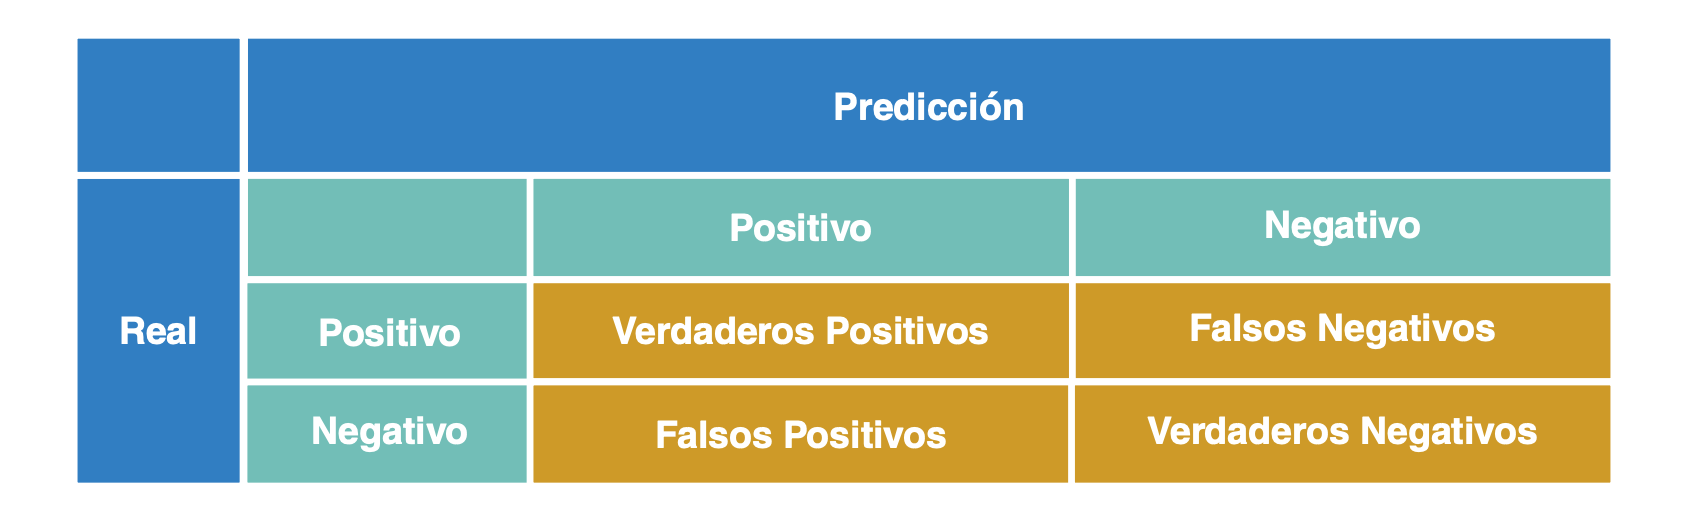
\includegraphics[width=\textwidth]{img/introduction/14_CM.png}
    \caption[Matriz de confusión]{\textbf{Matriz de confusión que ilustra la evaluación del rendimiento de un modelo de clasificación.} Los cuadrantes muestran verdaderos positivos, falsos negativos, falsos positivos y verdaderos negativos, permitiendo comparar predicciones con resultados reales. Imagen creada con BioRender \cite{biorender2025}.}
    \label{fig:CM}
\end{figure}

A partir de estos valores, se derivan varias métricas que ofrecen una perspectiva más profunda sobre el desempeño del modelo \cite{ferri2009experimental}.

%%% TPR %%%
La Tasa de Verdaderos Positivos (TVP), también conocida como sensibilidad, se define como la proporción de casos positivos que han sido correctamente identificados por el modelo:

\begin{equation}
   \text{TVP} = \frac{VP}{VP + FN} 
\end{equation}
\myequations{Cálculo de la Tasa de Verdaderos Positivos}

Esta métrica es esencial, ya que indica la capacidad del modelo para detectar correctamente instancias de la clase positiva.

%%% FPR %%%
La Tasa de Falsos Positivos (TFP) se refiere a la proporción de casos negativos que han sido incorrectamente clasificados como positivos:

\begin{equation}
    \text{TFP} = \frac{FP}{FP + VN}
\end{equation}
\myequations{Cálculo de la Tasa de Falsos Positivos}

La TFP es importante porque puede tener implicaciones significativas en situaciones donde las consecuencias de un falso positivo son graves, como en escenarios médicos.

%%% TNR %%%
La Tasa de Verdaderos Negativos (TVN), también conocida como especificidad, se define como la proporción de casos negativos que han sido correctamente identificados:

\begin{equation}
    \text{TVN} = \frac{VN}{VN + FP}
\end{equation}
\myequations{Cálculo de la Tasa de Verdaderos Negativos}

La TVN complementa a la TFP y es crucial para evaluar la efectividad del modelo en la identificación de instancias negativas.

%%% FNR %%%
La Tasa de Falsos Negativos (TFN) se refiere a la proporción de casos positivos que han sido incorrectamente clasificados como negativos:

\begin{equation}
    \text{TFN} = \frac{FN}{VP + FN}
\end{equation}
\myequations{Cálculo de la Tasa de Falsos Negativos}

Esta métrica es particularmente relevante en contextos donde es crítico identificar la clase positiva, como en diagnósticos médicos.


La \textit{Accuracy} es una de las métricas más comunes utilizadas para evaluar modelos de clasificación. Se define como la proporción de predicciones correctas sobre el total de instancias analizadas:

\begin{equation}
    \text{Accuracy} = \frac{VP + VN}{VP + VN + FP + FN}
\end{equation}
\myequations{Cálculo de la \textit{Accuracy}}

La medición de la \textit{accuracy} es intuitiva y fácil de interpretar, lo que la hace popular en diversas aplicaciones. Sin embargo, es importante tener en cuenta que su utilidad puede verse afectada en escenarios de clases desbalanceadas, donde un modelo podría lograr una alta \textit{accuracy} simplemente al predecir la clase mayoritaria.

En problemas de clasificación multiclase (es decir, cuando un modelo debe asignar instancias a una de tres o más categorías posibles), la \textit{accuracy} convencional puede no ser la mejor opción para evaluar el rendimiento de un modelo. Esto se debe a que, en muchos casos, los conjuntos de datos pueden estar desbalanceados, es decir, algunas clases pueden tener muchas más instancias que otras. En tales circunstancias, un modelo podría lograr una alta \textit{accuracy} simplemente al predecir la clase mayoritaria, sin tener en cuenta cómo se desempeña en las otras clases. Aquí es donde la \textit{Balanced Accuracy} (BA) se presenta como una alternativa más adecuada. Esta métrica se define como el promedio de la sensibilidad (o tasa de verdaderos positivos) y la especificidad (o tasa de verdaderos negativos):

\begin{equation}
    \text{BA} = \frac{1}{n} \sum_{i=1}^{n} \frac{\text{VP}_i}{\text{VP}_i + \text{FN}_i}
\end{equation}
\myequations{Cálculo de la \textit{Balanced Accuracy}}

\begin{itemize}
    \item Donde $\text{VP}_i$ es el número de verdaderos positivos para la clase $i$, $\text{FN}_i$ es el número de falsos negativos para la clase $i$ y $n$ es el número total de clases.
\end{itemize}


La BA ofrece una evaluación más equitativa del modelo, haciendo hincapié en su capacidad para manejar adecuadamente cada clase, independientemente de su frecuencia en el conjunto de datos. Esto permite identificar con mayor claridad las debilidades y fortalezas del modelo en relación con cada clase. En resumen, la BA no solo proporciona una imagen más completa del rendimiento del modelo en contextos de clasificación multiclase, sino que también ayuda a minimizar el impacto de las clases desbalanceadas en los resultados. Al adoptar esta métrica, se busca asegurar que el modelo sea realmente eficaz en la clasificación de todas las clases, no solo en aquellas que son más frecuentes, haciendo así una evaluación más robusta y justa del rendimiento del modelo.

El AUC (Area Under the ROC Curve) es una medida que se utiliza para evaluar la capacidad de un modelo de clasificación para discriminar entre las clases positiva y negativa. Se deriva de la curva ROC (Receiver Operating Characteristic), que representa gráficamente la TVP frente a la TFP a diferentes umbrales de decisión. El AUC se puede computar a partir de los puntos de la curva ROC. La fórmula aproximada para el AUC se puede expresar como:

\begin{equation}
    \text{AUC} = \sum_{i=1}^{n-1} \left( TFP_i - TVP_{i-1} \right) \cdot TFP_i
\end{equation}
\myequations{Cálculo de la \textit{Area Under the ROC Curve}}

\begin{itemize}
    \item Donde $TFP_i$ y $TFP_{i-1}$ son las tasas de falsos positivos en los puntos $(i)$ y $(i-1)$, respectivamente. $TVP_i$ es la tasa de verdaderos positivos en el punto $(i)$. Y $n$ es el número total de puntos en la curva ROC.
\end{itemize}

El AUC se puede interpretar como la probabilidad de que el modelo clasifique correctamente una instancia positiva por encima de una instancia negativa elegida aleatoriamente. Su valor oscila entre 0 y 1, donde un AUC de 1 indica un modelo perfecto que distingue perfectamente entre las clases, un AUC alrededor de 0,5 indica que el modelo no tiene poder discriminativo y clasifica al azar, y un AUC menor de 0,5 indica un rendimiento inferior al azar.

\textbf{Validación}

Para evaluar y evitar el sobreajuste de los modelos en la fase de entrenamiento, es necesario realizar procesos de validación. Esta validación es el proceso de evaluar el rendimiento de un modelo en datos que no se utilizaron durante el entrenamiento, lo que permite estimar su capacidad para generalizar a nuevas muestras no vistas. Dentro de estas técnicas de validación, las más utilizadas son el \textit{holdout}, la validación cruzada (CV) y la \textit{Nested cross-validation} (NCV).

La validación por \textit{holdout} es el enfoque más sencillo, donde el conjunto de datos se divide en un conjunto de entrenamiento y uno de prueba. El modelo se entrena en la primera partición y se evalúa en la segunda. Si bien es computacionalmente eficiente, la estimación del rendimiento puede ser muy variable, especialmente en conjuntos de datos pequeños. \cite{kohavi1995study}.

La estrategia de CV mejora el método \textit{holdout} al dividir el conjunto de datos múltiples veces para reducir la variabilidad en las estimaciones de rendimiento. Por ejemplo, la \textit{k-fold} CV es un tipo de validación en la que el conjunto de datos se divide en (\textit{k}) subconjuntos de igual tamaño. En cada una de las (\textit{k}) iteraciones, un subconjunto se retiene como conjunto de validación, mientras que los restantes (\textit{k} – 1) subconjuntos se utilizan para el entrenamiento; cada observación sirve exactamente una vez como muestra de validación. El rendimiento medio a través de los subconjuntos proporciona una comprensión más estable y completa de cómo se espera que funcione el modelo en datos independientes \cite{kohavi1995study}.

La NCV lleva el proceso de evaluación un paso más allá al abordar el riesgo de un posible sesgo durante la optimización de hiperparámetros y la selección de modelos. Como se  representa en la Figura \ref{fig:NCV}, esta técnica implica dos capas de CV: un bucle interno, que se utiliza exclusivamente para seleccionar los hiperparámetros óptimos y las configuraciones del modelo, y un bucle externo, que proporciona una estimación imparcial del rendimiento de generalización del modelo final. Al separar estrictamente la optimización del modelo de la estimación de rendimiento, la NCV asegura que la evaluación no se vea influenciada inadvertidamente por las decisiones tomadas durante la optimización de hiperparámetros, reflejando así una expectativa de rendimiento más realista.

\begin{figure}[h]
    \centering
    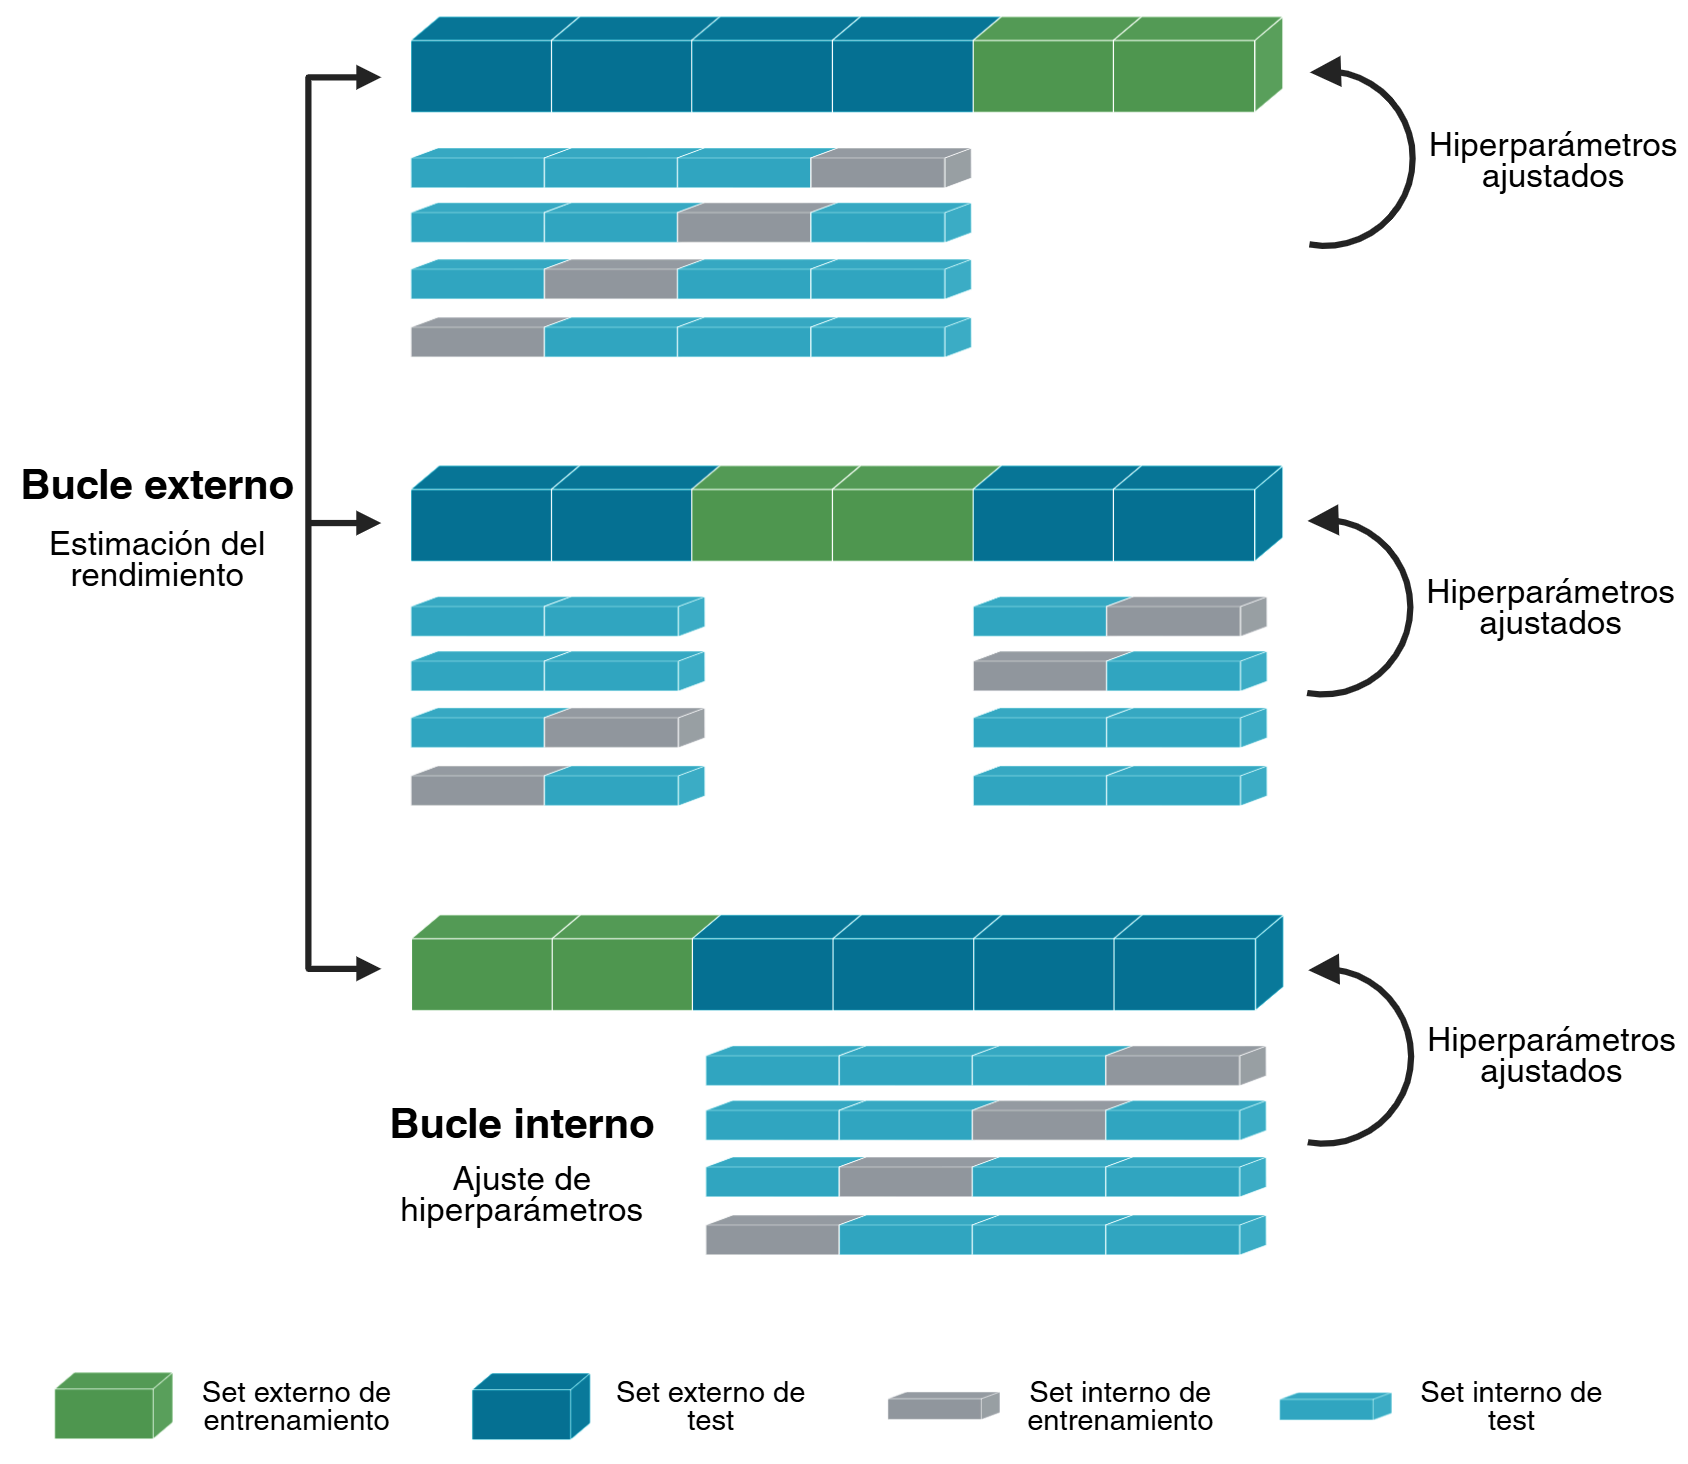
\includegraphics[width=\textwidth]{img/introduction/15_NCV.png}
    \caption[Representación de una \textit{Nested cross-validation}]{\textbf{Esquema de NCV.} El bucle externo se utiliza para estimar el rendimiento del modelo, mientras que, el bucle interno se centra en el ajuste de los hiperparámetros. Se garantiza una evaluación robusta mediante partición en conjuntos de entrenamiento y test en ambos bucles. Imagen creada con BioRender \cite{biorender2025}.}
    \label{fig:NCV}
\end{figure}

La aplicación de aprendizaje supervisado en datos del microbioma tiene como objetivo principal crear modelos predictivos a partir de patrones microbianos. Estos modelos pueden clasificar a pacientes, identificar firmas metagenómicas o predecir la respuesta a tratamientos. La combinación de modelos lineales, basados en \textit{kernels} y en árboles, junto con métricas de rendimiento y estrategias de validación robustas como la NCV, asegura que los hallazgos sean sólidos y generalizables, consolidando esta aproximación como una herramienta prometedora en la investigación de biomarcadores potenciales en este ámbito.

Aunque las técnicas de ML permiten identificar subgrupos, patrones y generar modelos predictivos, el rendimiento de estos modelos depende significativamente de la calidad de las características utilizadas. Los datos del microbioma se caracterizan por su alta dimensionalidad, donde el número de taxones es mucho mayor que el de muestras. Esta característica puede introducir ruido, aumentar la complejidad computacional y dificultar la interpretabilidad de los resultados. Para mitigar estos problemas, la siguiente sección se enfoca en las técnicas de reducción de la dimensionalidad aplicadas en esta Tesis Doctoral.

\subsection{Técnicas de reducción de la dimensionalidad}

La reducción de dimensionalidad se refiere al proceso de transformar datos de alta dimensión en un espacio de menor dimensión, conservando la estructura y las relaciones esenciales presentes en los datos. En la investigación de microbioma, frecuentemente se generan datos mediante métodos de secuenciación que producen miles de características (OTUs o ASVs), lo que plantea desafíos significativos para la visualización e inferencia estadística.

Los métodos tradicionales pueden volverse ineficaces o propensos al sobreajuste cuando se enfrentan a un espacio de características tan amplio. Por lo tanto, las técnicas de reducción de dimensionalidad buscan simplificar estos conjuntos de datos complejos, ya sea transformando las características originales en un nuevo conjunto de variables latentes (extracción de características) o seleccionando un subconjunto de las variables originales (selección de características) que sean más informativas para los análisis posteriores. En la práctica, la aplicación de estas técnicas no solo mejora la eficiencia computacional, sino que también contribuye a descubrir patrones biológicos subyacentes y posibles biomarcadores que podrían estar oscurecidos por el ruido y la redundancia en los datos en bruto \cite{guyon2003introduction}.



\subsubsection{Extracción de características}

La extracción de características es el proceso de transformar las variables originales en un nuevo conjunto de variables (a menudo denominadas componentes o factores latentes) que son representativas de la estructura subyacente de los datos. El objetivo principal de la extracción de características es capturar la variación o los patrones incrustados en los datos, desechando al mismo tiempo el ruido y la información redundante. Esto se logra a través de transformaciones matemáticas que buscan resumir las características originales en menos dimensiones. Una ventaja central de la extracción de características es que a menudo revela estructuras latentes que pueden corresponder a procesos biológicos subyacentes.


La transformación de las matrices de conteos de abundancia microbiana en representaciones de baja dimensión permite no solo simplificar la complejidad del conjunto de datos, sino también identificar patrones latentes, diferencias entre comunidades y posibles biomarcadores asociados a estados patológicos o condiciones ambientales. En este contexto, destacan métodos como la Descomposición en Valores Singulares (SVD) y el Análisis de Componentes Principales (PCA). Estos métodos han ganado una amplia aceptación debido a su capacidad para reducir la dimensionalidad, preservando al mismo tiempo la información biológica relevante.

\paragraph{Descomposición en Valores Singulares}

La SVD es una técnica de descomposición matricial que descompone una matriz de datos $A$ en tres matrices: $U$, $\Sigma$ y $V^T$ (Figura \ref{fig:SVD}). La matriz $U$ contiene vectores que describen patrones en las filas, mientras que $V^T$ hace lo mismo para las columnas. La matriz $\Sigma$ contiene los valores singulares, que indican la importancia de los patrones latentes. Estos valores, ordenados de mayor a menor, muestran qué patrones capturan más variación en los datos. Los primeros valores singulares suelen ser los más significativos, y al enfocarse en ellos, podemos simplificar los datos conservando gran parte de la información relevante. Esto permite reducir la dimensionalidad de manera efectiva, revelando estructuras ocultas y simplificando el análisis de conjuntos de datos complejos.

\begin{figure}[h]
    \centering
    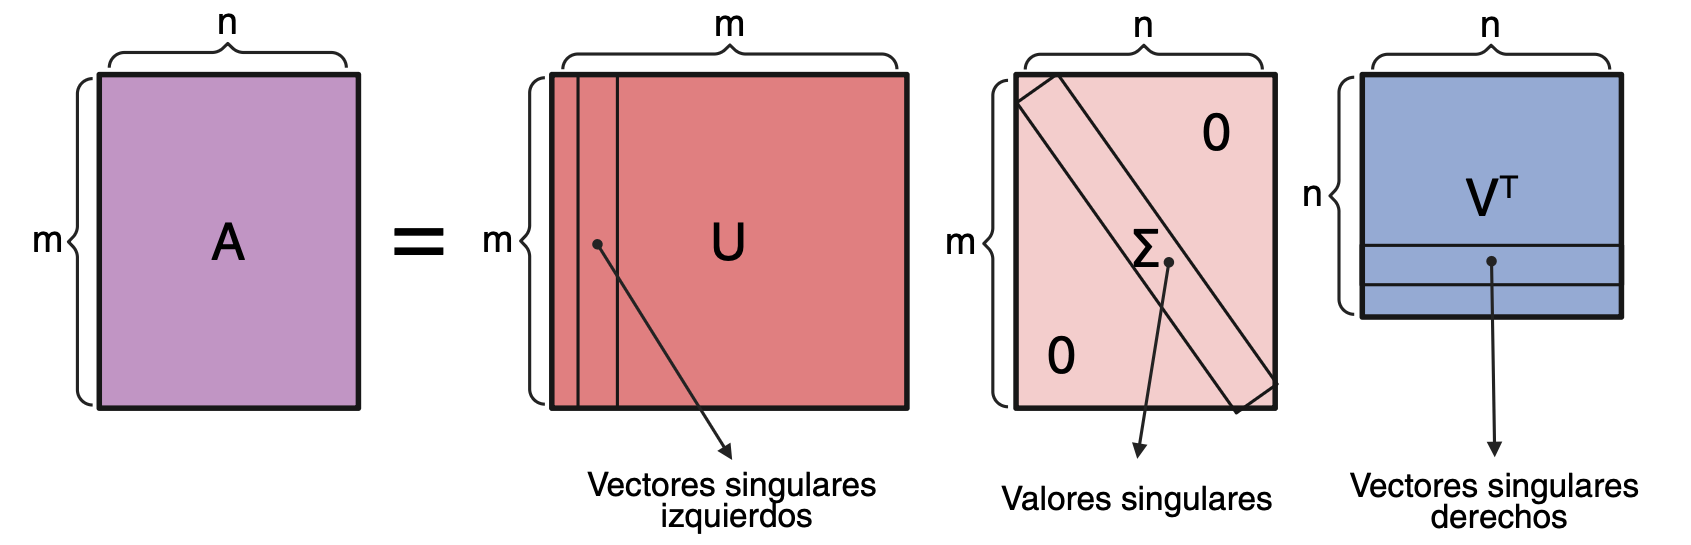
\includegraphics[width=\textwidth]{img/introduction/SVD.png}
    \caption[Descomposición en Valores Singulares]{\textbf{Diagrama de SVD.} Descomposición de la matriz $A$. Aquí, $U$ es una matriz ortogonal de m x m, $\Sigma$ es una matriz diagonal de m x n con los valores singulares en la diagonal, y $V^T$ es la traspuesta de una matriz ortogonal de n x n.}
    \label{fig:SVD}
\end{figure}

En el análisis de microbioma, SVD se utiliza tanto para descomponer tablas de abundancia de OTUs o ASVs como para asignar pesos a cada taxón en función de su contribución a la variación global. Esto es esencial para interpretar las diferencias entre muestras y entender la ecología microbiana.


\paragraph{Análisis de Componentes Principales }

Como se representa en la Figura \ref{fig:PCA}, el PCA transforma un conjunto de variables que pueden estar correlacionadas en un nuevo conjunto de variables linealmente no correlacionadas llamadas componentes principales. Se calculan de manera que la primera componente captura la mayor parte de la varianza de los datos, mientras que cada componente subsiguiente captura la máxima varianza restante, manteniendo la ortogonalidad entre ellas. Esto permite representar los datos en un espacio con menor dimensionalidad, conservando la mayor cantidad de información posible.


\begin{figure}[h]
    \centering
    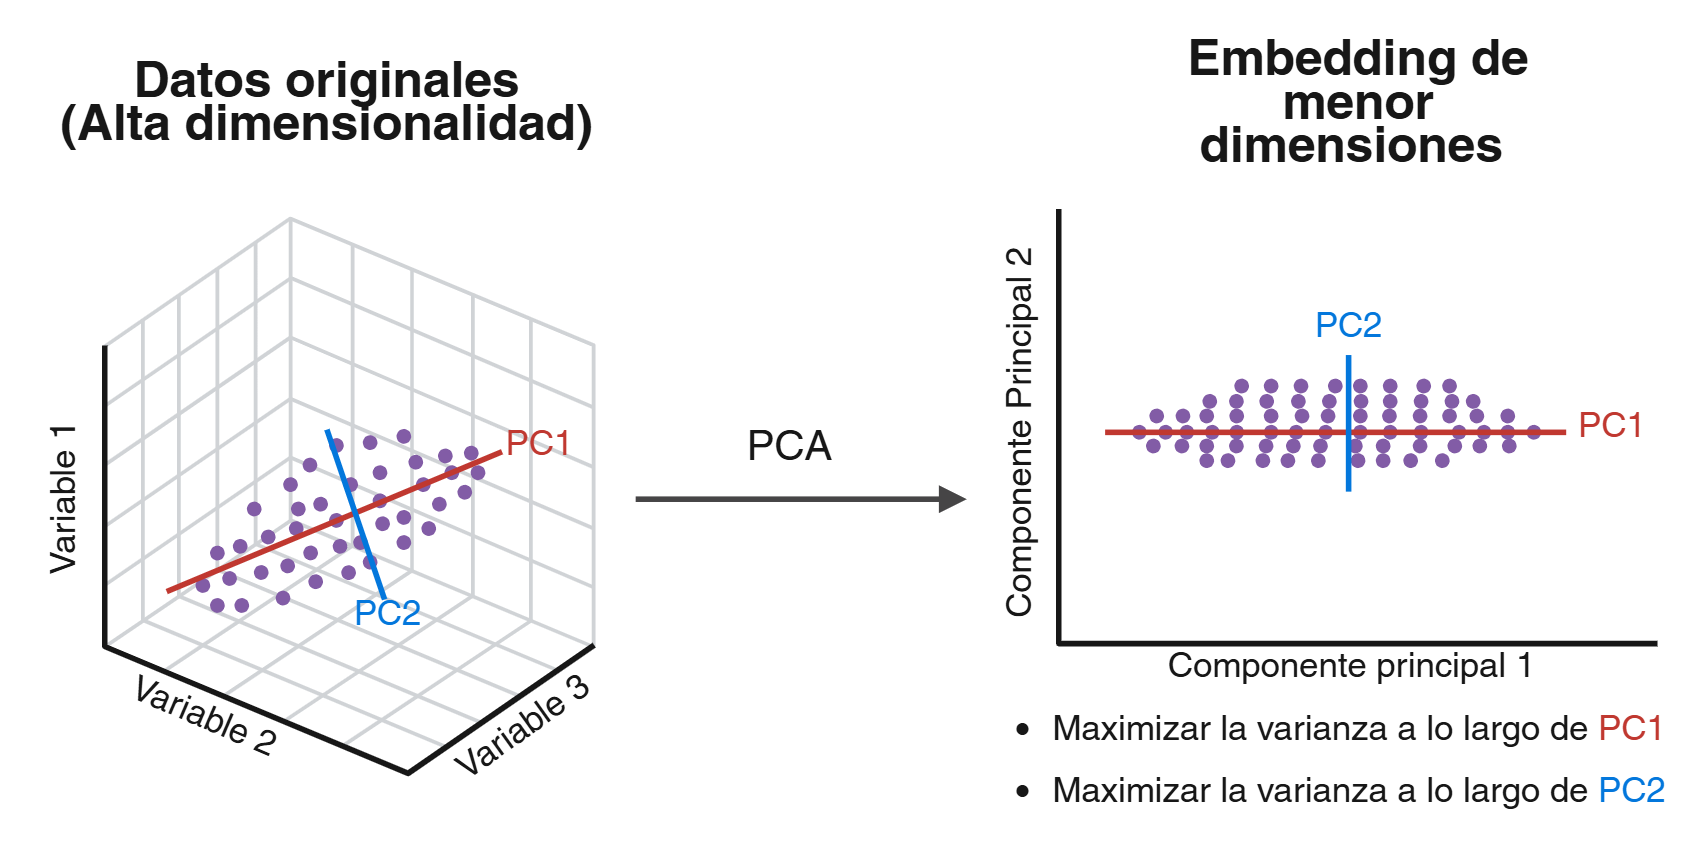
\includegraphics[width=\textwidth]{img/introduction/16_PCA.png}
    \caption[Análisis de Componentes Principales]{\textbf{Diagrama de PCA.} Los datos originales de alta dimensionalidad se transforman en un espacio de menor dimensión utilizando componentes principales (PC1, PC2), maximizando la varianza a lo largo de estas nuevas dimensiones.  Imagen creada con BioRender \cite{biorender2025}.}
    \label{fig:PCA}
\end{figure}


No obstante, a pesar de su amplia aplicación, el PCA presenta ciertas limitaciones en el contexto de datos de microbioma. Las suposiciones fundamentales que subyacen al PCA incluyen la linealidad en las relaciones entre las variables, la ortogonalidad de las componentes principales y que la estructura de varianza en los datos es un indicador adecuado para la señal biológica subyacente. Sin embargo, los datos de microbioma se caracterizan por su escasez y composicionalidad, y si estas características no se abordan cuidadosamente durante el preprocesamiento, el PCA puede conducir a patrones engañosos que no representan verdaderamente las diferencias biológicas subyacentes. Para abordar estos inconvenientes, se ha propuesto el PCA ajustado mediante transformaciones composicionales (por ejemplo, transformaciones CLR o distancias de Aitchison), que permiten obtener resultados con mayor coherencia e interpretación biológica, preservando la estructura composicional de los datos.

A pesar de estas limitaciones, el PCA sigue siendo una herramienta poderosa para la reducción de dimensionalidad, ofreciendo los beneficios duales de simplicidad computacional y facilidad de interpretación cuando se aplica adecuadamente.

\subsubsection{Selección de caracterísitcas}

A diferencia de la extracción de características, los métodos de selección de características no transforman los datos originales en nuevas variables compuestas, sino que seleccionan un subconjunto de características del conjunto de datos inicial que son más propensas a ser informativas para explicar el resultado o fenómeno biológico de interés. En el descubrimiento de biomarcadores de microbioma, la motivación principal detrás de la selección de características es reducir el espacio de características de alta dimensión al eliminar variables redundantes, irrelevantes o ruidosas, aumentando así la interpretabilidad y reduciendo el riesgo de sobreajuste en modelos predictivos posteriores. La selección de características también es especialmente valiosa en casos donde las características originales tienen significados biológicos claros, como los taxones microbianos o familias de genes, que pueden quedar enmascarados si son transformados por algoritmos de extracción de características \cite{saeys2007review}.

Actualmente se diferencian 3 tipos de técnicas de selección de características: métodos de \textit{filter}, \textit{wrapper} o \textit{embedded} (Representados en la Figura \ref{fig:FS}). La elección del método depende del contexto del análisis y los recursos computacionales disponibles.

\begin{figure}[h]
    \centering
    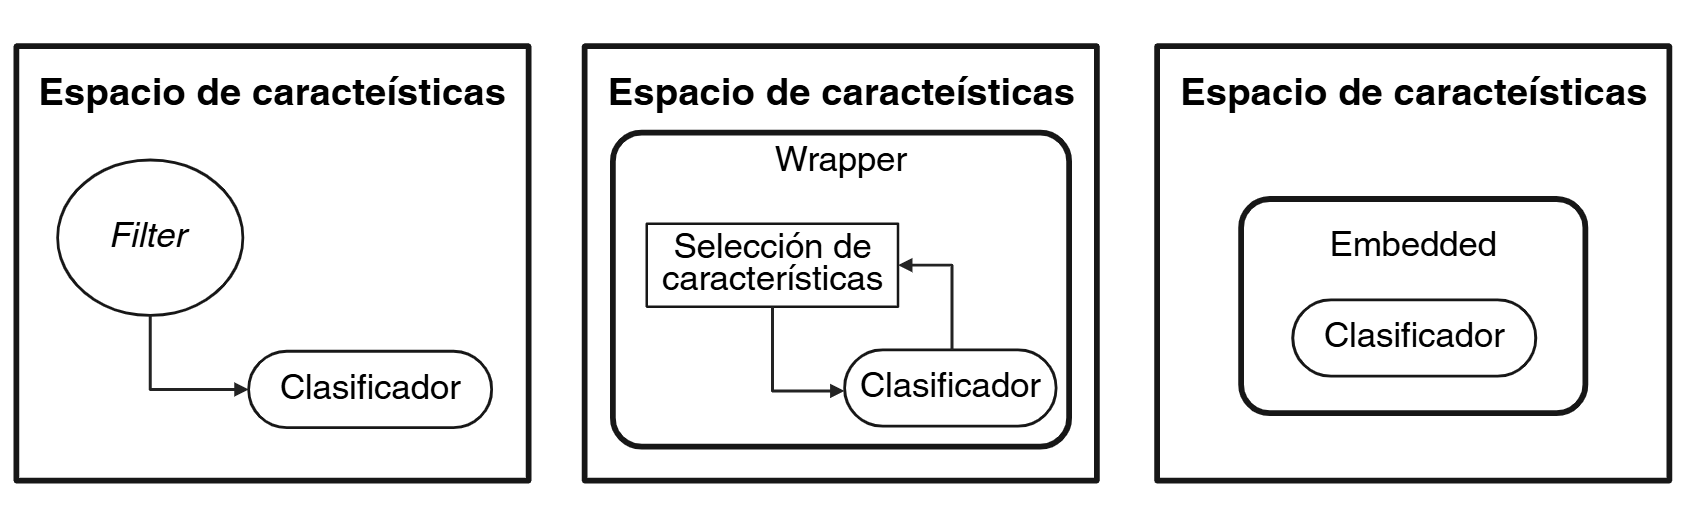
\includegraphics[width=\textwidth]{img/introduction/18_FS.png}
    \caption[Enfoques de selección de características]{\textbf{Enfoques de selección de características.} \textit{Filter} selecciona características antes del clasificador. \textit{Wrapper} evalúa iterativamente con el clasificador. \textit{Embedded} integra la selección directamente en el proceso de entrenamiento del modelo.  Imagen creada con BioRender \cite{biorender2025}.}
    \label{fig:FS}
\end{figure}


\paragraph{Técnicas \textit{filter}}

Los métodos \textit{filter} son uno de los enfoques más populares para la selección de características en estudios de microbioma, debido a su eficiencia computacional y a la interpretabilidad directa de las características seleccionadas. Estas técnicas operan de manera independiente de cualquier algoritmo de aprendizaje al clasificar las características en función de criterios estadísticos predefinidos. 

Las técnicas de \textit{filter} pueden aplicarse utilizando un enfoque univariante o multivariante. En los métodos de \textit{filter} univariantes, cada característica se evalúa de manera independiente, lo que los hace computacionalmente poco costosos, pero que puede pasar por alto interacciones entre características. Las técnicas univariantes suponen que el efecto de cada característica sobre el resultado es independiente de las demás y no tienen en cuenta la redundancia entre características altamente correlacionadas. Por el contrario, los enfoques de \textit{filter} multivariantes intentan considerar las interacciones y la redundancia de las características.

En la práctica, los métodos de \textit{filter} tienen la ventaja de ser agnósticos al modelo y pueden utilizarse como un paso preliminar para reducir la dimensionalidad antes de aplicar métodos más intensivos en computación. Su suposición subyacente es que las características con fuertes asociaciones individuales con el resultado son probablemente informativas cuando se utilizan juntas.

Las técnicas \textit{filter} son las más empleadas en el desarrollo de la presente Tesis Doctoral, principalmente debido a la claridad en la interpretación de sus resultados y a la reducción del tiempo computacional requerido. En situaciones donde la prioridad es comprender los mecanismos biológicos subyacentes, no es recomendable utilizar técnicas que dependan del tipo de algoritmo aplicado para justificar los resultados. En este contexto, las técnicas \textit{filter}, al ser independientes del tipo de algoritmo seleccionado, permiten el entrenamiento de diversos modelos utilizando los subconjuntos de variables obtenidos. Esto facilita una interpretación más clara de las interacciones biológicas en los datos de microbioma, contribuyendo a una mejor comprensión del fenómeno estudiado.

\paragraph{Técnicas \textit{wrapper}}

Los métodos \textit{wrapper} abordan la selección de características evaluando el rendimiento predictivo de un clasificador o modelo de regresión en diferentes subconjuntos de características. Estas técnicas utilizan el rendimiento de un algoritmo de aprendizaje como función objetivo y suelen realizar una búsqueda iterativa (ya sea a través de selección hacia adelante secuencial, eliminación hacia atrás, algoritmos genéticos o eliminación recursiva de características) para identificar el subconjunto óptimo de características que proporciona el mejor rendimiento del modelo.

Las técnicas \textit{wrapper} tienen la ventaja de optimizar directamente el rendimiento del modelo predictivo. Sin embargo, son computacionalmente intensivas porque requieren entrenamiento y validación repetidos del modelo para diferentes combinaciones de características. Además, dado que están estrechamente ligadas a modelos predictivos específicos, las características seleccionadas por un método \textit{wrapper} pueden no generalizar bien a otros algoritmos de aprendizaje. La suposición clave subyacente a los métodos \textit{wrapper} es que el mejor subconjunto de características para un clasificador también funcionará bien en un esquema de clasificación similar, una suposición que podría no mantenerse si el modelo es altamente sensible a las características de entrada específicas.

\paragraph{Técnicas \textit{embedded}}

Los métodos de selección de características \textit{embedded} integran el proceso de selección en la fase misma de entrenamiento del modelo. Estas técnicas penalizan la inclusión de demasiadas características durante el proceso de ajuste del modelo, reduciendo así a cero los coeficientes de características menos importantes y eliminándolas efectivamente del modelo.

Estos métodos logran un equilibrio entre la eficiencia computacional de los métodos \textit{filter} y la optimización del rendimiento de las técnicas \textit{wrapper}, dado que la selección de características se realiza simultáneamente con la construcción del modelo. Aunque estos métodos son generalmente más eficientes que las técnicas \textit{wrapper}, su rendimiento depende de la correcta especificación del parámetro de regularización o de la estructura del modelo subyacente. En muchos casos, los métodos incorporados se utilizan junto con una CV para asegurar que las características seleccionadas sean robustas y no artefactos de sobreajuste a los datos de entrenamiento. 
%%%%%%%%%%%%%%%%%%%%%%%%%%%%%%%%%%%%%%%%%%%%%%%%%%%%%%%%%
%%%%%%%%%%%%%%%%%         FUNDAMENTOS              %%%%%%%%%%%%%%%%%%%%%%
%%%%%%%%%%%%%%%%%%%%%%%%%%%%%%%%%%%%%%%%%%%%%%%%%%%%%%%%%


\chapter{Objetivos}
\label{chap:objectives}

\chapterintro{
El desarrollo de esta Tesis Doctoral está motivado por la necesidad de avanzar en el campo de la bioinformática aplicada a la salud humana. En el contexto actual, la identificación de biomarcadores microbianos es fundamental para mejorar el diagnóstico y pronóstico de diversas enfermedades. Este capítulo detalla los objetivos que guían este trabajo de investigación, fundamentando la importancia de cada uno en el ámbito científico y médico.}


El objetivo principal de esta Tesis Doctoral es el \textbf{desarrollo y aplicación de metodologías bioinformáticas para la identificación de biomarcadores microbianos asociados a enfermedades humanas}. Esto se aborda con futuros fines diagnósticos, utilizando el análisis de datos de microbioma obtenidos mediante secuenciación masiva y técnicas de Machine Learning.


Por consiguiente, a partir del objetivo principal se plantean los siguientes objetivos específicos:
\begin{itemize}

    \item \textbf{Evaluar la capacidad predictiva y de estratificación del microbioma humano}. Este objetivo se centra en el desarrollo, implementación y optimización de flujos de trabajo bioinformáticos que permitan el análisis de datos de secuenciación masiva del microbioma. Se busca establecer la viabilidad computacional de utilizar las abundancias taxonómicas como variables de entrada para entrenar modelos de ML. La finalidad es construir modelos robustos capaces de clasificar y estratificar a los pacientes para fines diagnósticos (distinción entre individuos sanos y enfermos) o pronósticos (predicción de la respuesta o no respuesta a un determinado tratamiento), facilitando la identificación de subgrupos con perfiles microbianos distintivos y determinando el potencial del microbioma en la medicina personalizada.
    
    \item \textbf{Explorar el papel del microbioma humano como fuente de biomarcadores}. Una vez establecida la capacidad predictiva del microbioma, este objetivo se centra en aprovechar la información generada para el descubrimiento de biomarcadores. Se utilizarán modelos de ML interpretables para extraer los taxones que mayor contribución tengan en la clasificación o predicción de estados clínicos. La finalidad es caracterizar estos biomarcadores microbianos clave y su asociación con diversas patologías, utilizando la información generada como base para nuevas investigaciones.

    \item \textbf{Validar los biomarcadores microbianos identificados mediante un análisis comparativo en cohortes clínicas independientes}. Este objetivo se centra en evaluar la consistencia y robustez de los biomarcadores identificados inicialmente en una cohorte principal mediante comparaciones in silico con datos de cohortes externas. Esta validación externa garantiza que los biomarcadores mantengan su relevancia y potencial clínico en diferentes contextos, fortaleciendo su aplicabilidad en estudios futuros.
    
\end{itemize}
%%%%%%%%%%%%%%%%%%%%%%%%%%%%%%%%%%%%%%%%%%%%%%%%%%%%%%%%%
%%%%%%%%%%%%%%%%%         ANTECEDENTES              %%%%%%%%%%%%%%%%%%%%%%
%%%%%%%%%%%%%%%%%%%%%%%%%%%%%%%%%%%%%%%%%%%%%%%%%%%%%%%%%


\chapter{Resultados}
\label{chap:results}

\chapterintro{En este capítulo, se muestran los resultados obtenidos a lo largo de esta Tesis Doctoral en forma de publicaciones indexadas en el \textit{Journal Citation Reports} (JCR). En conjunto, dan respuesta a los objetivos enumerados en el capítulo anterior.}

Este capítulo inicia con un primer trabajo \cite{paper1} donde se analizan datos del microbioma fecal de pacientes con SM o DT2 para identificar taxones diferenciales. Posteriormente, en el segundo trabajo \cite{paper2}, se avanza hacia el campo predictivo, aplicando una metodología de ML para evaluar el potencial del microbioma en el diagnóstico temprano de DT1. Finalmente, el tercer trabajo \cite{paper3} analiza el microbioma vaginal en el contexto de la VB para caracterizar mejor los fenotipos, mejorar el subtipado y así encontrar asociaciones con el tratamiento. La Figura \ref{fig:papersGA} ofrece un resumen gráfico que sintetiza estas tres publicaciones.


\begin{figure}[h]
    \centering
    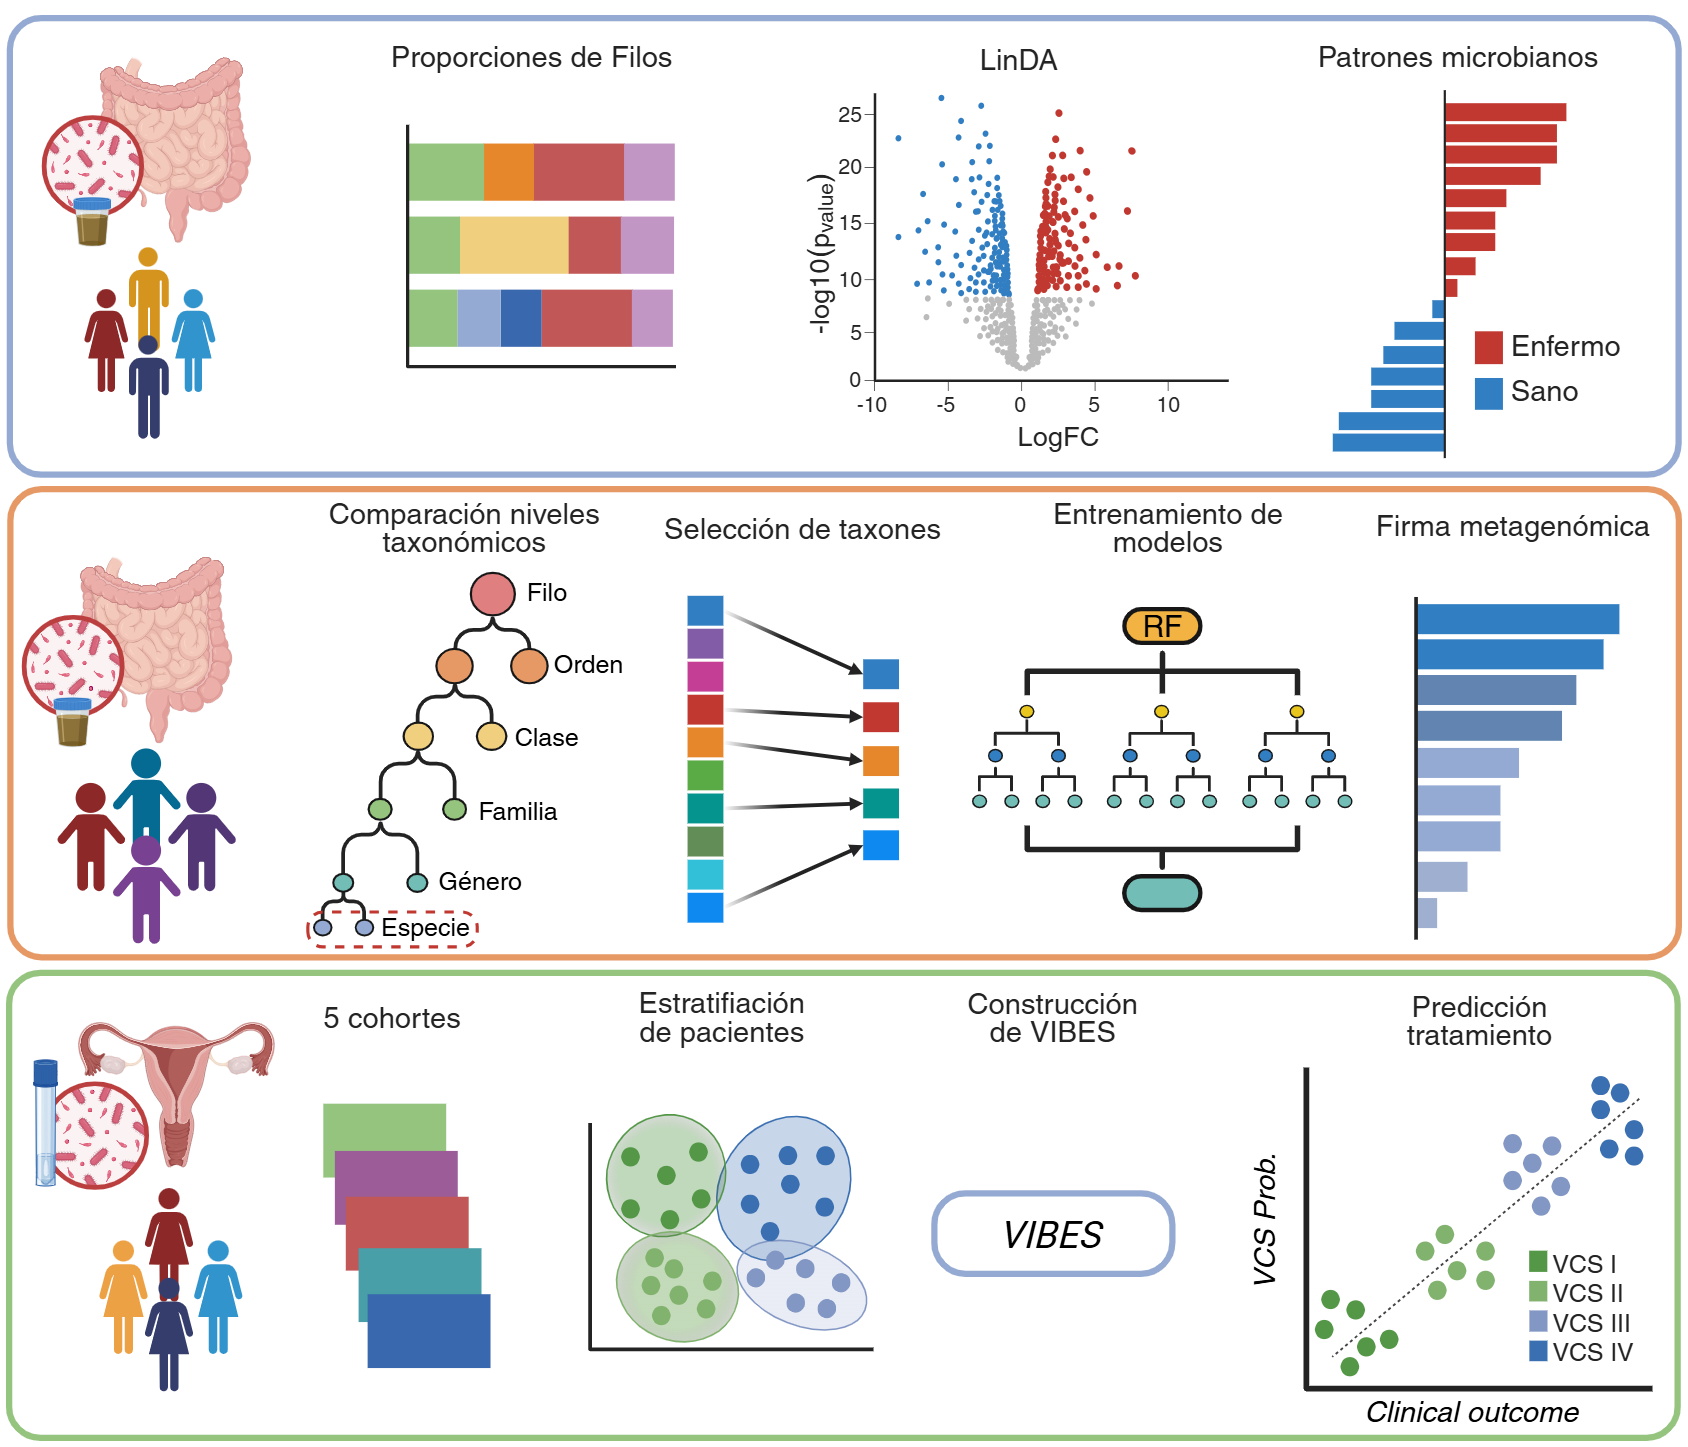
\includegraphics[width=\textwidth]{img/results/GA.png}
    \caption[\textit{Abstract} gráfico de las 3 publicaciones]{\textbf{\textit{Abstract} gráfico de las 3 publicaciones que conforman la Tesis Doctoral.} El primer trabajo \cite{paper1} analiza el microbioma intestinal en el contexto de SM y DT2. En el segundo trabajo \cite{paper2} se estudia el microbioma instestinal en infantes sanos y con DT1. Finalmente en el tercer trabajo \cite{paper3} se estudia el microbioma vaginal asociado a VB. Imagen creada con BioRender \cite{biorender2025}.}
    \label{fig:papersGA}
\end{figure}



\section{Búsqueda de patrones microbianos característicos de enfermedades metabólicas}


El incremento global de enfermedades metabólicas complejas como SM y DT2 destaca la necesidad urgente de comprender sus orígenes y mecanismos subyacentes \cite{saklayen2018global, zimmet2016diabetes}. Una línea prometedora de investigación se centra en el microbioma intestinal, dado su papel potencial en la regulación metabólica. Los desequilibrios en la composición del microbioma podrían ser fundamentales en la patogénesis de estas enfermedades al influir en factores como la inflamación y la resistencia a la insulina. Esta investigación se inspira en la posibilidad de que el análisis del microbioma pueda ayudar a identificar biomarcadores diagnósticos. Con esta motivación, este estudio se diseñó para identificar taxones con abundancias diferenciales que pudieran servir como biomarcadores en estas patologías, utilizando para ello la cohorte del proyecto IBEROBDIA \cite{IBEROBDIA_project}.

Este trabajo parte de dos esquemas de comparación: por un lado, individuos sanos frente a pacientes con SM; y por otro, una clasificación más detallada que distingue entre individuos sanos, prediabéticos y aquellos con DT2. El estudio del SM y DT2 desde perspectivas diferenciadas permite un análisis más preciso del impacto que pueden tener en el microbioma intestinal. El estudio del SM se caracteriza por su naturaleza como conjunto de factores de riesgo que predicen un mayor desarrollo hacia condiciones más graves, como DT2. Estudiar directamente los efectos del SM facilita la identificación de cambios microbianos que podrían ser utilizados como señales tempranas o indicadores de riesgo. Por otro lado, evaluar DT2 desde un punto de vista gradual (desde individuos sanos, pasando por prediabéticos, hasta diabéticos) ofrece una visión detallada de cómo los desequilibrios en el microbioma se desarrollan a lo largo del proceso de la enfermedad. Este enfoque diferencial no solo ayuda a identificar patrones específicos de disbiosis asociados a cada etapa, sino que también permite explorar posibles intervenciones y respuestas del microbioma a lo largo del avance de la enfermedad.

En primera instancia, se realizó un análisis exploratorio considerando las abundancias relativas a nivel de filo, así como la diversidad \textit{alfa} y \textit{beta}. Posteriormente, se empleó LinDA \cite{zhou2022linda} para analizar las abundancias relativas a nivel de género y especie. Los resultados de este trabajo indican que, a nivel de filo, es posible hallar indicadores asociados a ambas patologías. En particular, la relación Bacteroidetes/Firmicutes muestra variaciones relevantes y, en el caso de DT2, se observa un enriquecimiento de Actinobacteriota. En el caso del SM, se identifican varios taxones del género \textit{Blautia} que están sobrerrepresentados en los pacientes que sufren de este síndrome. En cuanto a la diabetes, se observa cómo taxones del género \textit{Bifidobacterium} están enriquecidos en pacientes sanos y cómo el taxón \textit{Dorea} (a través de \textit{Dorea longicatena}) está considerablemente sobrerrepresentado en los pacientes prediabéticos y diabéticos.

Los resultados obtenidos indican que los cambios en el microbioma intestinal están claramente asociados con SM y DT2, lo que refuerza hallazgos previos sobre la relación entre los organismos microbianos y estas patologías \cite{valdes2018role, lynch2016human, gurung2020role}. Sin embargo, nuestro trabajo ha identificado taxones que no han sido destacados en la literatura actual, como \textit{Parabacteroides merdae}, \textit{Lachnospiraceae GCA-900066575} y \textit{Defluviitaleaceae UCG-011}, lo que sugiere la necesidad de explorar otros géneros y/o especies que puedan estar asociadas con la enfermedad. Aunque existe la posibilidad de que algunos de los taxones identificados no tengan un efecto causal, podrían proporcionar información valiosa sobre la enfermedad como indicadores de diagnóstico.

El código fuente para reproducir todos los análisis, junto con la documentación, está disponible en GitHub (https://github.com/MALL-Machine-Learning-in-Live-Sciences/IBEROBDIA) y Zenodo (https://doi.org/10.5281/zenodo.14051704). Además, los datos brutos y los datos clínicos están disponibles en formato phyloseq en Figshare (https://doi.org/10.6084/m9.figshare.26063020.v1).

Fui coautor principal del trabajo liderando la parte computacional del mismo. Realicé el preprocesado y los análisis de los datos, construí las figuras y las tablas, y escribí el manuscrito. La información de participación de los otros autores está descrita en el artículo.

\includepdf[pages = -]{back/paper1}

\section{Evaluación de la capacidad predictiva del microbioma en Diabetes Tipo 1}


La creciente incidencia de DT1 en pacientes pediátricos en países desarrollados ha impulsado la necesidad de explorar sus causas y fundamentos \cite{mayer2017incidence, manuwald2021trends}. Hasta ahora, gran parte de la investigación en DT1 se ha centrado en factores genéticos y ambientales, pero el microbioma intestinal puede desempeñar un papel crucial en el desarrollo de la enfermedad. Comprender esta relación podría revelar biomarcadores microbianos útiles para el diagnóstico temprano y la intervención preventiva. Estudiar DT1 desde un enfoque metagenómico en infantes resulta crítico, ya que el desarrollo microbiológico durante los primeros años de vida puede determinar la susceptibilidad a enfermedades autoinmunitarias. Este trabajo tiene como objetivos entrenar un modelo predictivo eficiente a partir de datos de abundancias y buscar una firma metagenómica con potencial para la clasificación de pacientes con DT1. Para alcanzar estos objetivos, el estudio se basó en los datos publicados y disponibles del proyecto DIABINMUNE \cite{diabimmune}.


En este trabajo, para investigar la relación entre el microbioma intestinal y DT1, se llevan a cabo dos análisis usando técnicas de ML. Primero, se realiza un análisis de clasificación para separar a los individuos sanos de aquellos con DT1. Posteriormente, se efectúa un análisis multiclase que incluye a individuos con seroconversión. Estos individuos se caracterizan por haber comenzado a desarrollar autoanticuerpos contra sus células beta pancreáticas, lo que indica que su sistema inmune ya inició el proceso autoinmune que puede llevar a DT1. Este análisis busca identificar cambios sutiles en el microbioma que podrían ocurrir antes de que la enfermedad se manifieste clínicamente, brindando una visión sobre las etapas intermedias en la progresión de DT1, donde las diferencias biológicas no son tan evidentes. A partir del número total de especies, se lleva a cabo un proceso de selección de características para reducir la dimensionalidad y mejorar el entrenamiento de los modelos. Este enfoque tiene como objetivo extraer y ordenar las especies según su importancia para clasificar pacientes sanos y diabéticos. De esta manera, buscamos determinar el número exacto de especies necesarias para entrenar un modelo cuyo rendimiento no mejore al añadir más especies.


Finalmente, se seleccionaron 25 especies como número óptimo para el análisis. Con estas especies, se evaluaron tres algoritmos: glmnet, SVM y RF. El algoritmo RF, entrenado con la abundancia de estas especies, mostró una \textit{accuracy} de 0,94 y un \textit{AUC} de 0,99, demostrando una gran capacidad para clasificar a los pacientes como sanos o con DT1. Entre las 25 especies, destacan 5 por su alta importancia en la clasificación entre ambas clases: \textit{Bacteroides uniformis}, \textit{Bacteroides dorei}, \textit{Prevotella copri}, \textit{Bacteroides vulgatus} y \textit{Bacteroides thetaiotaomicron}. Además, al reutilizar tanto el algoritmo como las especies para incluir una tercera clase intermedia, se constató que el modelo mantiene su robustez con un \textit{accuracy} cercano a 0,94.

Los resultados obtenidos sugieren una fuerte asociación entre diversas especies bacterianas y la susceptibilidad a DT1. La identificación de una firma metagenómica robusta no solo confirma algunos vínculos esperados \cite{higuchi2018intestinal, medina2019dietary, wu2020metagenomic}, sino que también revela especies que podrían haber sido subestimadas o pasadas por alto en trabajos anteriores, como \textit{Anaerotruncus colihominis}, \textit{Clostridium symbiosum} y \textit{Clostridium bartlettii}, entre otros. Aunque algunos de los taxones identificados pueden no tener un efecto causal, podrían proporcionar información valiosa sobre la enfermedad como indicadores de diagnóstico.

El código fuente para reproducir todos los análisis, junto con la documentación, está disponible en GitHub (https://github.com/MALL-Lab/MLMicrobiomeT1D). Los datos utilizados en este trabajo pueden descargarse del proyecto DIABINMMUNE (https://diabimmune.broadinstitute.org/diabimmune/t1d-cohort/resources/16s-sequence-data). El Shiny creado para la exploración interactiva de los resultados está disponible en el repositorio de Shiny (https://diegofedreira.shinyapps.io/shinyapp/). La imagen de Docker para recrear los análisis y el Shiny está alojada en Docker Hub (https://hub.docker.com/r/cafernandezlo/mlmicrobiomet1d).

Fui el autor principal de este trabajo. Realicé el diseño experimental, ejecuté la metodología de ML, construí las figuras y las tablas y escribí el manuscrito. La información de participación de los otros autores está descrita en el artículo.

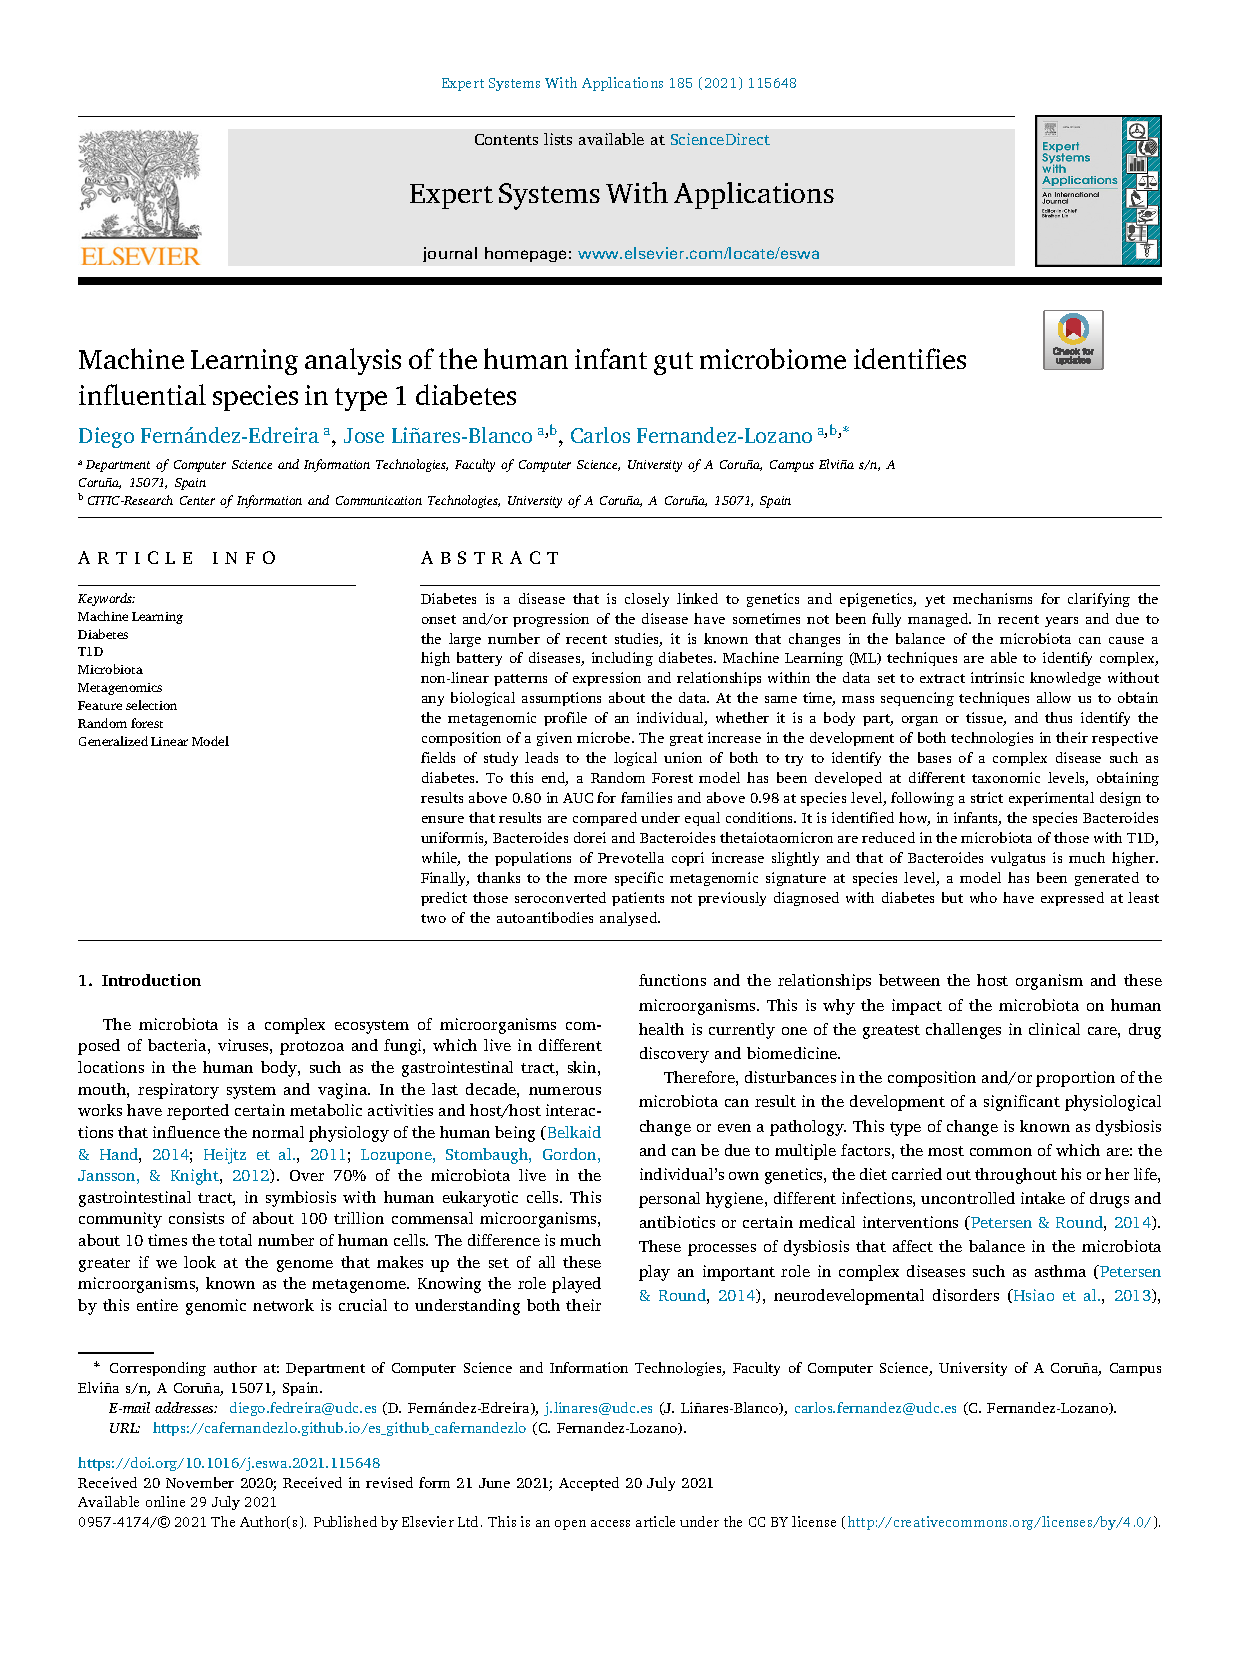
\includepdf[pages = -]{back/paper2}

\section{Caracterización del microbioma vaginal en el contexto de Vaginosis Bacteriana}

La VB es una de las infecciones más comunes en mujeres en edad reproductiva, pero su diagnóstico se ve complicado por la heterogeneidad de sus fenotipos y las respuestas variables al tratamiento. Un enfoque metagenómico permite explorar la disbiosis subyacente a esta condición, abriendo la puerta a una mejor clasificación y, con ello, a tratamientos más personalizados. Por tanto, este último trabajo tuvo como objetivo mejorar la caracterización de los fenotipos de VB y enriquecer la clasificación de esta enfermedad. Para ello, se emplean 5 cohortes de microbioma vaginal depositadas en el ENA \cite{leinonen2010european}.

Para realizar la caracterización y el subtipado de pacientes, se partió de una cohorte formada por casi 400 pacientes \cite{ravel2011vaginal}. Se utilizó el método de \textit{clustering} por consenso CCP \cite{wilkerson2010consensusclusterplus} para la división de los pacientes según sus perfiles microbianos. Como resultado, se definieron 4 subtipos (VCS I-IV), los cuales se comprobaron y validaron en el resto de las cohortes. Estos subtipos se emplearon para entrenar un modelo de tipo \textit{Elastic Net}, denominado VIBES (https://mall-lab.github.io/VIBES-docs/), capaz de generalizar en cohortes externas y distribuido como paquete en R. A partir de una firma metagenómica predefinida, VIBES estima la probabilidad de pertenencia de cada paciente a los distintos subtipos, lo que permite analizar sus puntuaciones en cohortes independientes. Finalmente, para comprobar la significancia biológica de los subgrupos obtenidos a través de VIBES, se realizó una comparación con un método de estratificación reconocido en el estado del arte, llamado VALENCIA \cite{france2020valencia}. Además de una comparación de subgrupos, se llevó a cabo un experimento para determinar si, integrando la información de ambos enfoques, se puede mejorar la predicción de un medicamento para VB, en comparación con usar ambos enfoques por separado.

Estos cuatro subgrupos están conformados por 20 especies, siendo taxones clave varias especies del género \textit{Lactobacillus}, y especies como \textit{Gardnerella vaginalis} y \textit{Atopobium vaginae}, entre otras. Posteriormente, se realizó una comparación con los subgrupos (CSTs) de VALENCIA, y resulta interesante observar que el subconjunto asintomático en VALENCIA se correspondió predominantemente al grupo VCS-I en nuestro análisis (caracterizado por mayores abundancias de \textit{Lactobacillus crispatus}). No obstante, también se identificaron diferencias significativas entre los dos sistemas de clasificación. En concreto, los grupos intermedios de VIBES, como VCS-II y VCS-III, muestran una gran heterogeneidad en comparación con los subtipos de CST. Esta discrepancia podría ser un indicador de que nuestro enfoque proporciona información adicional a VALENCIA. Finalmente, para comprobar la utilidad de VIBES (y medir su diferencia con VALENCIA en un caso práctico), se planteó la hipótesis de usar las variables obtenidas por ambos enfoques para predecir la respuesta al metronidazol mediante modelos de ML. Se observó que, al integrar la información de ambos enfoques, se logra un rendimiento de 0,76 de \textit{accuracy}, mejorando el rendimiento que se consigue usando enfoques individuales (0,7 de \textit{accuracy}), lo que indica que VIBES estaría captando información biológica complementaria a VALENCIA.


En conclusión, la identificación de los cuatro subgrupos VCS I-IV mediante el enfoque de \textit{clustering} por consenso enriquece la comprensión de la diversidad microbiana en el ecosistema vaginal. La comparación de los grupos obtenidos con este enfoque frente a los que se obtienen usando VALENCIA sugiere que nuestro enfoque proporciona información adicional y complementaria. Además, los resultados obtenidos al integrar ambos enfoques en la predicción de la respuesta al metronidazol evidencian este hecho. Estos hallazgos no solo contribuyen a la evaluación y al manejo de la VB, sino que también abren nuevas vías para la investigación de estrategias terapéuticas más adaptadas a las características individuales de cada paciente.

El código fuente para reproducir todos los análisis, junto con la documentación, está disponible en GitHub (https://github.com/MALL-Lab/VIBES-analysis). El modelo VIBES está disponible en GitHub (https://github.com/MALL-Lab/VIBES). Los datos de secuenciación de todas las cohortes (SRA022855, SRA051298, PRJNA208535, PRJNA797778 y PRJNA302078) pueden consultarse a través de sus respectivos números de acceso en el ENA.

Fui coautor principal del trabajo. Realicé el tratamiento y preprocesamiento de los datos, ejecuté la metodología de ML, construí las figuras y las tablas, y escribí el manuscrito. La información de participación de los otros autores está descrita en el artículo.

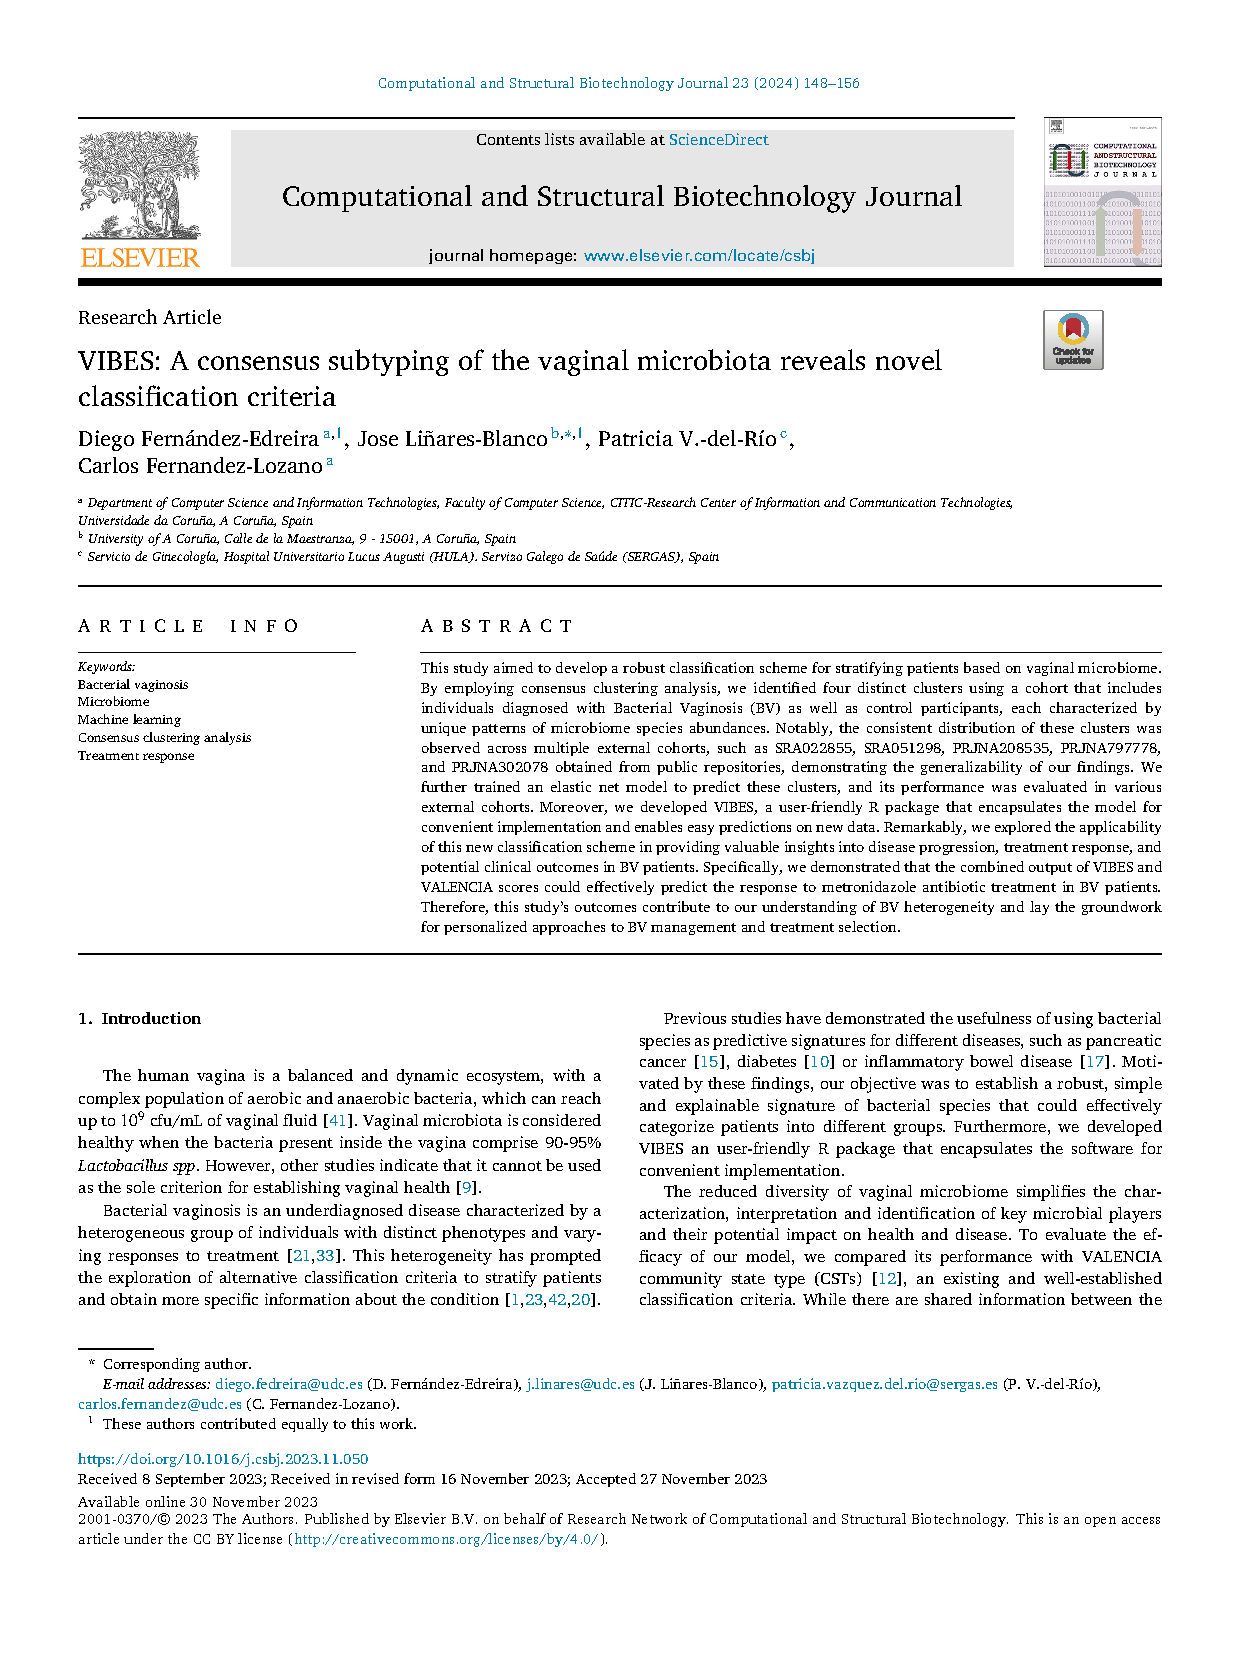
\includepdf[pages = -]{back/paper3}
%%%%%%%%%%%%%%%%%%%%%%%%%%%%%%%%%%%%%%%%%%%%%%%%%%%%%%%%%
%%%%%%%%%%%%%%%%%%%         SOLUCION              %%%%%%%%%%%%%%%%%%%%%%%
%%%%%%%%%%%%%%%%%%%%%%%%%%%%%%%%%%%%%%%%%%%%%%%%%%%%%%%%%


\chapter{Discusión}
\label{chap:discussion}

\chapterintro{
En conjunto los tres artículos que conforman esta Tesis Doctoral estudian, tanto el potencial del microbioma como fuente de biomarcadores, como la aplicación de técnicas de ML para el análisis de datos del microbioma con el fin de apoyar procesos diagnósticos. Siguiendo el hilo argumental de los tres artículos y los resultados obtenidos, esta sección aborda aspectos específicos y transversales generados a lo largo de la investigación.
}



Esta Tesis Doctoral explora el microbioma como fuente de biomarcadores con potencial diagnóstico y emplea técnicas computacionales para convertir perfiles microbianos en señales útiles para la clasificación y la estratificación clínica. El uso de datos 16S rRNA se justifica por su accesibilidad, estandarización y amplia disponibilidad pública; cualidades que favorecen estudios a gran escala, validaciones externas y reproducibilidad, sin establecer una jerarquía frente a WGS, sino una elección pragmática alineada con objetivos y recursos. Bajo este marco, se integraron análisis de abundancia diferencial, selección de características y Machine Learning con un procesamiento explícitamente composicional, a fin de respetar la naturaleza relativa de los conteos y evitar pérdidas informativas por submuestreo.



En primera instancia, se decidió estudiar las enfermedades presentadas a lo largo de la Tesis Doctoral debido a su conocida y fuerte conexión con algún componente microbiano. En el caso de las enfermedades metabólicas, estas tienen una relación directa con el tracto intestinal y su correcto funcionamiento, un ambiente que presenta una gran carga microbiana. En cuanto a la VB, se sabe que la patogénesis de la enfermedad tiene un gran porcentaje microbiano. Al estudiar estas enfermedades \cite{paper1, paper2, paper3}, es fundamental considerar la naturaleza de las muestras utilizadas. Las muestras fecales, al ser deslocalizadas, reflejan una visión general del microbioma intestinal a lo largo de todo el tracto digestivo. Esto es crucial para enfermedades sistémicas y complejas como el SM o DT1/2, donde el impacto puede deberse a interacciones a gran escala dentro del sistema digestivo. En contraste, las muestras localizadas, como los hisopos vaginales, ofrecen un análisis más directo de un ecosistema microbiano específico y menos heterogéneo. Dado que el microbioma vaginal es menos diverso, las alteraciones en su composición son más fáciles de asociar directamente con alteraciones específicas en la salud vaginal. Este diseño permitió poner a prueba la versatilidad del marco metodológico en escenarios con distinta señal microbiana esperable: en VB se anticipaban patrones comunitarios estables y clínicamente relevantes; en DT1/DT2, firmas predictivas robustas, pero con relaciones más difusas, moduladas por múltiples covariables. Los resultados fueron coherentes con estas premisas.


Metodológicamente, se optó por ASVs para maximizar la resolución y reproducibilidad, y por DADA2 como método de inferencia por su modelado explícito de los errores provenientes de la secuenciación y su independencia del conjunto de muestras \cite{callahan2017exact, nearing2018denoising, caruso2019performance, prodan2020comparing}. Al mismo tiempo, la evidencia reunida en esta Tesis Doctoral muestra que OTUs y ASVs pueden converger en señales comunitarias comparables cuando el preprocesamiento es cuidadoso: en \cite{paper3}, un modelo de \textit{clustering} basado en OTUs se validó en datos procesados con ASVs, mostrando que los patrones comunitarios principales se mantienen entre ambos enfoques; y en \cite{paper2}, las OTUs son suficientes para extraer una firma predictiva con alto rendimiento. Esto está en línea con evidencias que indican que, pese a diferencias en riqueza o asignación taxonómica, la topología del \textit{clustering} y las señales globales tienden a ser comparables \cite{chiarello2022ranking}. Aunque la agrupación puede fusionar secuencias e incrementar la riqueza, las OTUs capturan patrones robustos a niveles superiores \cite{liu2023independent}. La elección, por tanto, debe alinearse con el objetivo: granularidad para detectar cambios sutiles (ASVs) o robustez comunitaria para clasificación (OTUs).


El procesamiento composicional fue clave; la mayor preocupación era mitigar la gran variabilidad en la profundidad de secuenciación entre muestras y representar fielmente las proporciones de los taxones microbianos. Frente a la rarefacción, la cual puede simplificar en exceso las comparaciones al eliminar datos potencialmente relevantes, transformaciones logarítmicas como CLR y métodos de abundancia diferencial compatibles (p. ej., LinDA) preservaron la información y aumentaron la sensibilidad \cite{gloor2016compositional, gloor2017microbiome, hong2022rarefy, zhou2022linda}. Gracias a ambos, en el primer trabajo \cite{paper1}, se extrajeron patrones significativos. En el caso de los otros trabajos \cite{paper2, paper3}, se comparó el rendimiento aplicando estas transformaciones frente a los datos crudos y se observó que el rendimiento se reducía al no aplicar dichas transformaciones. Además, en este último trabajo, aplicar estas transformaciones ayudó a reducir la variabilidad entre los diferentes enfoques utilizados (OTUs vs ASVs) a lo largo de las distintas cohortes. Aunque una parte de la literatura \cite{lambeth2015composition, dash2023functional, siptroth2023variation, chen2018vaginal, onywera2021predictive} sigue empleando normalizaciones que ignoran la composicionalidad, la evidencia acumulada en esta Tesis Doctoral respalda un tratamiento composicional consistente.



Con el objetivo de maximizar el espacio de descubrimiento, se adoptó un enfoque dirigido por datos en lugar de uno basado en conocimiento. El enfoque dirigido por conocimiento depende de hipótesis preexistentes, vías biológicas conocidas o bases de datos curadas. Aunque proporciona interpretabilidad biológica y es un excelente complemento para confirmar hallazgos, limita la capacidad de descubrimiento a lo ya conocido \cite{dakal2025advanced}. El enfoque dirigido por datos opera sin depender de suposiciones biológicas. Esto es crucial en la búsqueda exploratoria de nuevos biomarcadores, ya que permite analizar datos brutos y descubrir patrones ocultos o no lineales \cite{hemmati2024using}. Al elegir una metodología guiada por este tipo de enfoque, se seleccionó el ML, ya que se deseaba utilizar una metodología que manejase, en cierta medida, la alta variabilidad, dispersión y complejidad del microbioma, y que además tuviese explicabilidad. En el estado del arte actual, se utilizan muchos enfoques basados en el conocimiento en el campo del microbioma \cite{chong2017computational, bauer2018network, luo2024progress}. Sin embargo, a lo largo de los tres trabajos \cite{paper1, paper2, paper3}, al analizar datos brutos en lugar de un subconjunto basado en conocimiento previo, hemos descubierto tanto taxones ya mencionados en la literatura como otros poco documentados o desconocidos en la patología de estudio. Esto abre la puerta a investigar el papel de estos taxones en el desarrollo de enfermedades y su potencial como biomarcadores.


Para afrontar el desafío de la alta dimensionalidad en los datos del microbioma, se han implementado filtros rigurosos (conteos totales y prevalencia de taxones) al extraer la tabla de taxones y se han aplicado técnicas de selección de características que permiten reducir el número de taxones considerados en la construcción de modelos de ML, las cuales han demostrado ser efectivas en este contexto \cite{segata2011metagenomic}. Actualmente, el problema de la dimensionalidad está presente en el estudio de datos procedentes del microbioma, ya que numerosos artículos en el estado del arte realizan algún tipo de selección de características \cite{beck2015machine, biassoni2020gut, bakir2021discovering, bakir2022inflammatory, chavarria2025using}. Esta selección de características desempeña un papel importante en el segundo trabajo de esta Tesis Doctoral \cite{paper2}. Este artículo emplea la selección de características para identificar las especies más relevantes capaces de diferenciar las muestras entre sano y DT1. La estrategia seguida fue utilizar una técnica de selección de características de filtrado, lo que permite medir la relevancia de cada una de las especies con las clases de interés, identificando así cuántas y qué especies utilizar para construir el modelo predictivo. Los resultados muestran un aumento significativo en el rendimiento de los modelos al seleccionar un subgrupo de especies del número total disponible.


La variabilidad biológica y técnica se abordó mediante estrategias de validación estrictas. Por un lado, en el caso del aprendizaje no supervisado, el enfoque CCP ha permitido la construcción de subgrupos robustos y generalizables. En el aprendizaje supervisado, la implementación de una NCV garantiza un modelo robusto y generalizable, minimizando el riesgo de sobreajuste \cite{varma2006bias}. Esto se refleja en los trabajos \cite{paper2, paper3}, donde, gracias a esta validación, se ha manejado la diversidad en los datos de entrada, permitiendo la construcción de modelos con poca dispersión en su rendimiento, independientemente del conjunto de entradas. Esto se traduce en un modelo con altas capacidades para clasificar pacientes entre sanos y DT1 en el trabajo \cite{paper2}, y en un modelo en el trabajo \cite{paper3} que es capaz de predecir los VCS, incluso cuando los datos de entrada provienen de fuentes heterogéneas.

La elección algorítmica se adecuó al nicho y la tarea: modelos robustos a la dispersión y no linealidades (RF, XGBoost) frente a escenarios complejos, y modelos lineales (glmnet) cuando la estructura era más separable y se priorizaba la interpretabilidad \cite{goodswen2021machine, Lin2023MicrobiomeObesitySignatures}. El rendimiento superior de algoritmos no lineales como RF en el contexto de la predicción de DT1 \cite{paper2} se debe principalmente a la necesidad de modelar interacciones complejas del ecosistema microbiano intestinal, las cuales se ven agravadas por una alta variabilidad interindividual y las interacciones anfitrión-huésped. En contraste, el uso efectivo de un modelo lineal, como glmnet, en la estratificación de pacientes en función de los perfiles del microbioma vaginal \cite{paper3} refleja la naturaleza relativamente estructurada y linealmente separable de las comunidades microbianas vaginales, donde se pueden delimitar características clave con precisión. Las diferencias en el contexto de la enfermedad y la heterogeneidad de los nichos microbianos son, por lo tanto, fundamentales para explicar por qué los métodos no lineales son superiores en un escenario, mientras que los modelos lineales son más efectivos en otro.


Como se ha mencionado, el microbioma humano es un ecosistema altamente dinámico que exhibe variabilidad temporal, tanto a nivel composicional como funcional. Esta característica, reconocida en la literatura, plantea desafíos para la clasificación confiable de enfermedades utilizando datos del microbioma \cite{aldars2021systematic}. Sin embargo, los resultados obtenidos en esta Tesis Doctoral \cite{paper2, paper3}, al igual que otros en el estado del arte \cite{eck2017robust}, han demostrado que, incluso utilizando solo una muestra por paciente para la clasificación de enfermedades, se pueden lograr resultados robustos. Este hecho sugiere que la robustez en la clasificación entre estados patológicos no depende de capturar cada fluctuación transitoria, sino más bien de detectar los marcadores microbianos persistentes y dominantes que diferencian estos estados \cite{mehta2018stability}.


En \cite{paper1}, los pacientes con SM mostraron un aumento en la relación Firmicutes/Bacteroidetes, en línea con la hipótesis clásica sobre obesidad y fenotipos metabólicos \cite{santos2019role, baghi2022evaluation}. Se destacó una mayor prevalencia de \textit{Blautia}, cuya contribución a la disfunción metabólica podría implicar inflamación y disrupción de la barrera intestinal; además, en estudios previos, su abundancia se asoció con mayor severidad del SM en la enfermedad del hígado graso no alcohólico \cite{Liu2021, shen2017gut, Wang2016}. El enfoque seguido permitió la identificación de nuevos taxones que podrían desempeñar un papel protector en el contexto del SM. En particular, se relacionó la especie \textit{Parabacteroides merdae} con los controles sanos. Aunque no ha sido extensamente estudiada en humanos, trabajos recientes en modelos murinos sugieren que esta especie podría desempeñar un rol beneficioso a través del catabolismo de aminoácidos de cadena ramificada, cuya acumulación se ha relacionado con un aumento del riesgo metabólico \cite{qiao2022gut}. Además, estudios previos han reportado una reducción de ciertas especies del género \textit{Parabacteroides} en individuos con SM \cite{cui2022roles}.

En la progresión a DT2 se observó un aumento de la relación Bacteroidetes/Firmicutes y una disminución de Actinobacteria. Asimismo, se observa una pérdida de productores de butirato como \textit{Bifidobacterium} \cite{larsen2010gut, wu2010molecular, le2013alterations} y de taxones poco conocidos en este contexto: \textit{Lachnospiraceae GCA-900066575} y \textit{Defluviitaleaceae UCG-011} (potenciales fermentadores de fibra y productores de AGCCs). Estudios muy recientes realizados en ratones señalan que \textit{GCA-900066575} se relaciona negativamente con niveles de glucosa en sangre en ayunas y la resistencia a la insulina \cite{liu2023vitamin}. Simultáneamente, se observó un incremento en los taxones asociados con la patogénesis, como \textit{Dorea}, \textit{Prevotella} y \textit{Dialister invisus}. En el caso específico de \textit{Dorea longicatena}, se ha encontrado que esta especie está enriquecida en pacientes con DT2. Se ha observado una correlación clínica significativa entre su presencia y el desarrollo de la enfermedad \citep{qin2014alterations}. En cuanto a \textit{Prevotella}, varios estudios han establecido una asociación entre un aumento de esta bacteria y la intolerancia a la glucosa, así como la diabetes gestacional \citep{zhang2013human, egshatyan2016gut, hasain2020gut}. Por otro lado, la especie \textit{Dialister invisus} se ha vinculado con un aumento de la permeabilidad intestinal y la diabetes \citep{maffeis2016association, zheng2018gut}.



El segundo trabajo \cite{paper2} muestra que la profundidad taxonómica del estudio es un factor determinante para capturar la señal asociada a la T1D. Se observa que el rendimiento de los tres algoritmos utilizados mejora a través de seis niveles taxonómicos, desde filo hasta especie, con mejoras del 30\% entre ambos niveles. Esto sugiere que la asociación con la enfermedad se basa en la dinámica o interacción entre especies, en lugar de en desequilibrios de niveles superiores. La firma metagenómica identificada se alinea con asociaciones previamente descritas a nivel de especie. \textit{Bacteroides dorei} se ha vinculado con la seroconversión y con etapas preclínicas de autoinmunidad \cite{davis2014bacteroides}. \textit{Prevotella copri} y \textit{Bacteroides vulgatus} se han asociado con perfiles metabólicos de resistencia a la insulina \cite{pedersen2016human}. En cuanto a \textit{Bifidobacterium animalis}, se han observado efectos favorables en ensayos clínicos (principalmente en DT2) sobre control glucémico y parámetros cardiometabólicos \cite{stenman2016probiotic, khiaolaongam2025bifidobacterium}. En el eje intestino-inmunidad, \textit{Bacteroides thetaiotaomicron} se ha asociado con fenotipos de enfermedad celíaca y presenta una capacidad inmunomoduladora relevante \cite{sanchez2010intestinal}. Por último, la dinámica de \textit{Escherichia coli} productora de amiloide se ha relacionado con vías prodiabéticas y con la seroconversión en cohortes pediátricas \cite{tetz2019type}. Los modelos RF entrenados con esta firma presentan un gran rendimiento (0,94 de \textit{accuracy}) tanto al clasificar entre individuos sanos y pacientes de DT1, como al añadir una clase intermedia de seroconvertidos. Esto sugiere una fuerte asociación entre estas especies bacterianas y la susceptibilidad a DT1.

En este contexto, la mayoría de los estudios describen alteraciones composicionales y funcionales asociadas a la seroconversión y DT1 \cite{vatanen2018human, kostic2015dynamics}. De forma similar, otros estudios poblacionales \cite{belteky2023infant} han aplicado algoritmos de ML (RF) para la clasificación de taxones en búsqueda de biomarcadores; sin embargo, no se detalla su rendimiento predictivo para poder comparar con este trabajo. Desde la publicación de este segundo trabajo, en los últimos años se han publicado diferentes estudios con nuevas cohortes de infantes (como PRJNA875929 \cite{belteky2023infant} y PRJNA702261 \cite{del2022gut}), dando pie a realizar estudios de metacohortes con enfoques similares al presentado en esta Tesis Doctoral, como es el caso de \cite{liu2024predicting}.



En el tercer trabajo \cite{paper3}, los subgrupos obtenidos mediante \textit{VIBES} (VCS I–IV) mostraron una alta estabilidad en la cohorte de descubrimiento, con un ARI medio de 0,914. Esto sugiere que la estratificación en cuatro grupos está determinada por la estructura intrínseca de los datos, y no por el tamaño muestral. Además, la distribución de los subtipos fue consistente en cinco cohortes externas. En la validación externa del modelo, la BA fue superior a 0.91 en todas las cohortes, y el \textit{kappa} fue mayor a 0,83.

Desde la perspectiva biológica, las betas del modelo cuantifican la contribución relativa de cada especie en el clasificador para determinar la pertenencia a un subtipo. VCS-I, dominado por \textit{Lactobacillus crispatus}, se asocia con eubiosis: producción elevada de ácido láctico, pH bajo y exclusión competitiva de patobiontes \cite{ravel2011vaginal, srinivasan2012bacterial}. VCS-II, con \textit{Lactobacillus iners} (junto con \textit{Aerococcus christensenii}, \textit{Campylobacter ureolyticus}, \textit{Staphylococcus haemolyticus}), sugiere un estado de transición o vulnerabilidad aumentada \cite{macklaim2011crossroads, holm2023lactobacillus}. En VCS-III, las betas relevantes incluyen \textit{Lactobacillus iners}, \textit{Prevotella bivia}, \textit{Campylobacter ureolyticus} y \textit{Finegoldia magna}. Las especies del género \textit{Prevotella} pueden elevar el pH mediante la producción de aminas biógenas (putrescina, cadaverina, trimetilamina) y amonio, favoreciendo el crecimiento de \textit{Gardnerella} y promoviendo la transición hacia la disbiosis \cite{miller2016lactobacilli, yeoman2013multi}. Finalmente, VCS-IV es el subtipo más heterogéneo, evidenciando altas betas para \textit{Atopobium vaginae}, \textit{Sneathia sanguinegens}, \textit{Mycoplasma hominis} y \textit{Campylobacter ureolyticus}, y en menor medida para \textit{Lactobacillus gasseri}. La especie \textit{Atopobium vaginae} está asociada a \textit{biofilms}, un elevado pH y recurrencias debido a su menor sensibilidad al metronidazol \cite{swidsinski2008adherent, bradshaw2006association}; mientras que \textit{Sneathia} expresa factores de virulencia con potencial inflamatorio \cite{fredricks2005molecular, harwich2012genomic}.

Metodológicamente, VIBES y VALENCIA ofrecen visiones complementarias. \textit{VALENCIA} utiliza \textit{k-nearest neighbors} y hasta 199 taxones (clase–especie) para clasificar en 5 CSTs/subclases \cite{france2020valencia}; VIBES emplea un conjunto de 20 especies para 4 subtipos. Las diferencias en algoritmo, espacio de características y estructura de clases permiten captar señales no redundantes: perfiles sanos/asintomáticos de VALENCIA tienden a mapear con VCS-I, mientras que CSTs como III, IV-A o V no se alinean de forma directa con VCS-II/III, aportando granularidad complementaria \cite{ravel2011vaginal}. En la cohorte longitudinal tratada con metronidazol, el modelo combinado (VALENCIA + VIBES) mejoró la predicción de respuesta frente a cada enfoque por separado, y los no respondedores se concentraron en VCS-IV (y en menor medida en VCS-III), lo que sugiere que los subtipos de VIBES añaden información clínica independiente y potencialmente accionable para la estratificación basada en microbioma.



Las principales limitaciones se relacionan con el tamaño y la distribución muestral en \cite{paper1}, la ausencia de validación pediátrica independiente equivalente en \cite{paper2} (debido a la falta de cohortes comparables) y la diversidad geográfica y el panel de especies compartidas en \cite{paper3}. Más allá de las particularidades de cada estudio, la investigación del microbioma enfrenta fuentes de variabilidad técnica. Estas fuentes surgen a lo largo del flujo de trabajo: la elección de la región del gen 16S rRNA, los kits de extracción de ADN, las tecnologías de secuenciación empleadas (Illumina, PacBio, Ion Torrent), la estrategia de agrupación seguida (OTUs frente a ASVs), el método bioinformático para realizar dicha agrupación y las bases de datos de referencia utilizadas para la asignación taxonómica.

En resumen, las principales contribuciones de la presente Tesis Doctoral se pueden sintetizar en cuatro ejes fundamentales: la capacidad del microbioma como fuente de biomarcadores, el gran potencial del uso de técnicas de ML en el análisis del microbioma, la identificación de posibles biomarcadores microbianos con potencial de aplicación clínica en el contexto de la DT1/DT2 y el SM, y el desarrollo de una nueva estrategia de estratificación del microbioma vaginal en el contexto de la VB. Estas aportaciones evidencian la utilidad práctica del enfoque propuesto, instando a continuar explorando el microbioma como una herramienta clave para la personalización de intervenciones médicas. Este compendio, en conjunto, sienta las bases para un futuro en el cual las tecnologías emergentes y la integración de datos complejos configuren el panorama de la investigación biomédica, aportando beneficios tangibles a la salud pública y a la práctica clínica moderna. En el futuro, es crucial avanzar hacia la integración de plataformas analíticas para unificar datos, combinando información del microbioma y del anfitrión para entender mejor las interacciones biológicas y sus implicaciones en la salud. Además, investigar el microbioma como barrera en la eficacia de tratamientos y analizar la resistencia antimicrobiana facilitarán el desarrollo de estrategias innovadoras.
%%%%%%%%%%%%%%%%%%%%%%%%%%%%%%%%%%%%%%%%%%%%%%%%%%%%%%%%%
%%%%%%%%%%%%%%%%         EXPERIMENTACION              %%%%%%%%%%%%%%%%%%%%%
%%%%%%%%%%%%%%%%%%%%%%%%%%%%%%%%%%%%%%%%%%%%%%%%%%%%%%%%%


\chapter{Conclusiones}
\label{chap:conclussions}

\chapterintro{
En este capítulo se presentan las conclusiones extraídas tras el desarrollo de la presente Tesis Doctoral. Las conclusiones se basan en los tres artículos presentados, así como en la investigación transversal realizada
}

Los resultados obtenidos de esta Tesis Doctoral han permitido formular las siguientes conclusiones:

\begin{enumerate}

\item En el trabajo \cite{paper1}, a partir de una formada por 79 pacientes con riesgo de sufrir DT2, se demuestra que, a nivel de filo, es posible identificar señales o indicadores de una patología potencial. En este caso, el ratio de Bacteroidetes/Firmicutes varía a lo largo de la progresión de SM y de DT2. A niveles más específicos, se revela que taxones del género \textit{Blautia}, \textit{Tyzzerella} y \textit{Dorea} están enriquecidos en el perfil microbiómico de pacientes que sufren SM. Por otro lado, se presenta que el perfil microbiómico de pacientes con DT2 se caracteriza por una mayor abundancia de taxones como \textit{Dorea}, \textit{Prevotella} y \textit{Dialister}.

\item En el trabajo \cite{paper2}, se ha obtenido una firma metagenómica compuesta por 25 especies capaz de identificar a pacientes diagnosticados con DT1. En esta firma destacan, por su importancia, taxones del género \textit{Bacteroides} y \textit{Prevotella}, que pueden servir como biomarcadores en el caso de la patología de DT1. Además, se pone de manifiesto que un modelo de RF entrenado con dichas especies tiene un poder predictivo capaz de clasificar a los pacientes en sanos, seroconvertidos (estadío intermedio) y afectados por DT1.

\item En el trabajo \cite{paper3}, se ha propuesto un nuevo enfoque de estratificación de pacientes con VB a partir de datos metagenómicos. Este subtipado presenta información complementaria cuando se compara con otros métodos de subtipado del estado del arte. Además, en el contexto de VB, cuando se utiliza la información extraída de este método de subtipado, se mejora la predicción de la respuesta al tratamiento con metronidazol.

\item Finalmente, la investigación desarrollada en esta Tesis Doctoral confirma el potencial del microbioma como fuente de biomarcadores clínicos en varias patologías. De manera paralela, se demuestra el potencial de utilizar técnicas de ML para la construcción de modelos predictivos, y la capacidad de dichas técnicas para lidiar con los obstáculos inherentes al tipo de dato que es el microbioma.

\end{enumerate}
%%%%%%%%%%%%%%%%%%%%%%%%%%%%%%%%%%%%%%%%%%%%%%%%%%%%%%%%%
%%%%%%%%%%%%%%%%%         FUTUROS DESA              %%%%%%%%%%%%%%%%%%%%%%
%%%%%%%%%%%%%%%%%%%%%%%%%%%%%%%%%%%%%%%%%%%%%%%%%%%%%%%%%


\chapter{Futuros desarrollos}
\label{chap:future}

A raíz de la realización de la presentes Tesis Doctoral, se presentan varias líneas de investigación que serían interesantes en futuros desarrollos para explotar la información que nos brinda el microbioma.


\textbf{Integración de plataformas de secuenciación para facilitar comparaciones y combinaciones de datos para obtener resultados más robustos y coherentes}


Como se ha expuesto en la presente Tesis Doctoral, cada tipo de secuenciación del microbioma presenta sus ventajas. Mientras que el 16S rRNA es más asequible, rápido y presenta menos contaminación del ADN del anfitrión, el WGS presenta mayor resolución taxonómica y no presenta un sesgo debido a la selección de primers.

En los últimos años ha surgido la idea de si los datos provenientes de ambos tipos de secuenciación se podrían integrar eficazmente, ya que esto habilitaría diversas posibilidades, como incrementar el número de muestras accesibles de estudios del microbioma y comparar los resultados obtenidos en uno de los tipos de secuenciación con los obtenidos en la plataforma complementaria. Esto se traduciría en un mayor poder estadístico y en una mayor reproducibilidad en el descubrimiento de posibles biomarcadores en el campo del microbioma.

Ante esta necesidad de armonizar datos provenientes de diferentes tecnologías de secuenciación, recientemente se ha desarrollado la base de datos GreenGenes2, que, a futuro, puede constituir una herramienta importante para la integración de secuenciación 16S rRNA y WGS. GreenGenes2 \cite{mcdonald2024greengenes2} se basa en la unificación de secuencias derivadas tanto de la secuenciación de 16S rRNA como de WGS, construyendo un árbol filogenético de referencia que integra información de ambas plataformas en un solo marco taxonómico coherente. Mediante su estrategia de homogeneización, esta base de datos permite que los taxones obtenidos en estudios basados en 16S rRNA se puedan comparar de manera directa con aquellos obtenidos mediante WGS, facilitando así la integración de conjuntos de datos heterogéneos y la realización de meta-análisis a gran escala \cite{mcdonald2024greengenes2}.

Sin embargo, la variabilidad técnica proveniente de los diferentes protocolos de secuenciación o de las diferencias de resolución taxonómica es un gran obstáculo para una integración efectiva. En esta línea, se ha realizado un primer trabajo en el que se ha explorado el comportamiento de varios métodos de reducción de \textit{batch-effect} para integrar ambas plataformas \cite{fernandez2024cross}. En este trabajo se observa cómo estos métodos pueden llegar a corregir de manera eficiente las diferencias entre ambas plataformas. Sin embargo, no es concluyente si la calidad o la integridad de la señal biológica se mantiene después de aplicar dichos métodos.

En resumen, el desarrollo de metodologías y tecnologías que permitan la integración de datos de secuenciación 16S y WGS, así como la adopción de herramientas unificadoras como GreenGenes2, serán claves para avanzar en el análisis computacional del microbioma humano y en la generación de biomarcadores clínicos. Estos esfuerzos fortalecerán la capacidad de realizar estudios multicohorte integrados, optimizarán la comparación entre diferentes plataformas de secuenciación y contribuirán a la construcción de un marco analítico robusto que sea aplicable en entornos clínicos.


\textbf{Integración con otros datos ómicos procedentes del microbioma para obtener una visión más detallada de la actividad y funcionalidad del microbioma}


El análisis composicional del microbioma ha permitido explicar un porcentaje significativo de la patogénesis de ciertas enfermedades. Sin embargo, como se ha comentado en esta Tesis Doctoral, el enfoque metagenómico por sí solo no refleja toda la actividad real de estos microorganismos. Es aquí donde la integración con datos procedentes de metatranscriptómica (que se enfoca en qué genes se están expresando), metaproteómica (que cuantifica proteínas expresadas) y metabolómica (que analiza el perfil de metabolitos) resulta fundamental para revelar el estado funcional real del microbioma.

Los datos multiómicos que ya se están generando permiten medir la actividad real del microbioma, evaluando rutas como la producción de ácidos grasos de cadena corta, el metabolismo de ácidos biliares o la biosíntesis de vitaminas; definir grupos funcionales y relaciones entre microbios con impacto clínico; vincular genes y cepas con fenotipos y fallos de tratamiento; relacionar metabolitos y proteínas microbianas con medidas del huésped (marcadores inmunes y clínicos) para priorizar mecanismos; construir modelos predictivos interpretables para estratificar pacientes y anticipar la respuesta terapéutica, y analizar la evolución temporal para detectar cambios de estado y señales tempranas de descompensación. En conjunto, pasar de las abundancias taxonómicas a las funciones activas y su efecto en el huésped mejora la explicación de la enfermedad y acerca estos análisis a la aplicación clínica.

En los próximos años, la integración de datos metagenómicos con otras capas ómicas permitirá pasar de descripciones composicionales a perfiles funcionales y dinámicos del microbioma en contextos fisiopatológicos. Se adoptarán marcos de integración y se desarrollarán flujos de trabajo bioinformáticos reproducibles y robustos, con el objetivo de establecer biomarcadores clínicos para la estratificación de pacientes y orientar intervenciones terapéuticas basadas en la modulación del microbioma. Este avance hacia enfoques multiómicos integrados se perfila como un paso decisivo que, a medio y largo plazo, mejorará el diagnóstico y optimizará el tratamiento de enfermedades complejas.
    
    
\textbf{Integración microbioma-anfitrión para entender mejor las interacciones biológicas y sus implicaciones en procesos patológicos}


Llegados a este punto, todavía es comprensible pensar que abordar únicamente los datos ómicos derivados del microbioma (metagenoma, metatranscriptoma, metaproteoma y metaboloma) no resulta suficiente para descifrar en su totalidad los mecanismos biológicos subyacentes a determinadas patologías. En este contexto, la integración de datos procedentes tanto del microbioma como del anfitrión (genómica, transcriptómica, proteómica, entre otros) se presenta como una estrategia fundamental para obtener una visión sistémica de los procesos patológicos. Esta aproximación, que combina los múltiples niveles de información de ambas partes, permite detectar interacciones críticas que, de otro modo, podrían pasar desapercibidas.

La justificación de integrar datos del anfitrión radica en que el fenotipo de una enfermedad se encuentra en la intersección entre la información hereditaria del paciente y las influencias ambientales, de las cuales el microbioma es uno de los componentes más dinámicos y moduladores. Diversos estudios han demostrado que el genoma del anfitrión y su expresión fenotípica afectan directamente la composición y el funcionamiento del microbioma; por ejemplo, determinadas variantes genéticas están estrechamente relacionadas con la abundancia de taxones microbianos específicos, lo que repercute en procesos como la respuesta inmune, el metabolismo y la inflamación. Asimismo, las modificaciones inducidas en el transcriptoma y proteoma del huésped, ya sea por respuestas inmunitarias o por cambios metabólicos, pueden modular la actividad microbiana y, a su vez, influir en el desarrollo de patologías complejas \cite{duan2025advances}. Para abordar estas interacciones bidireccionales, es necesario el desarrollo de enfoques computacionales que permitan la integración simultánea de diferentes plataformas.

Un ejemplo revelador corresponde a los estudios en pacientes con cáncer, en los que se ha observado que la composición del microbioma puede influir en la eficacia de la inmunoterapia. La integración de perfiles metagenómicos con análisis del transcriptoma y proteoma tumoral ha permitido identificar biomarcadores que predicen la respuesta al tratamiento, lo que abre la puerta a intervenciones que combinan escenarios de microbiota dirigida con terapias convencionales \cite{goyal2025understanding}. Otro campo en el que la integración de datos del anfitrión y el microbioma ha mostrado resultados prometedores es el de la sepsis. Estudios recientes han empleado enfoques multiómicos para combinar datos de la expresión génica del huésped, perfiles proteómicos y datos metagenómicos, lo cual ha permitido distinguir entre infecciones bacterianas y virales en tiempo real, identificando biomarcadores que pueden predecir de manera temprana la progresión hacia cuadros de sepsis grave \cite{lu2025multi}.

En conjunto, la integración microbioma-huésped constituirá un eje clave de los futuros desarrollos: mejorará la identificación y validación de biomarcadores clínicos, permitirá modelos mecanísticos más precisos y favorecerá estrategias terapéuticas personalizadas que modulen tanto la respuesta del huésped como la composición y la función del microbioma. Esta línea de trabajo acercará los análisis multiómicos a la práctica clínica y optimizará la estratificación y el tratamiento de enfermedades complejas.


\textbf{Análisis del papel del microbioma en la resistencia a tratamientos terapéuticos} 


La compleja interacción entre el microbioma humano y los tratamientos farmacológicos constituye un área de investigación en rápida expansión, en la que se ha evidenciado que tanto el microbioma intestinal como el microbioma asociado a tejidos (por ejemplo, el microambiente tumoral) pueden actuar como barreras que impiden que algunos fármacos alcancen sus objetivos terapéuticos. El concepto de farmacomicrobiómica abarca la capacidad del microbioma para modificar, inactivar o incluso reactivar los fármacos mediante una serie de mecanismos que incluyen, entre otros, la captación de los compuestos, la secreción de metabolitos que alteran su estructura química y la modulación de la respuesta inmunitaria del huésped.

El microbioma puede actuar como barrera frente a fármacos a través de diferentes mecanismos directos e indirectos. Por ejemplo, en estudios experimentales se ha evidenciado que ciertas bacterias poseen la capacidad de secuestrar fármacos, resultando en menores concentraciones del compuesto en el lumen intestinal. Esta captación puede ser especialmente crítica en el caso de medicamentos con ventana terapéutica estrecha, ya que pequeñas variaciones en la biodisponibilidad pueden marcar la diferencia entre eficacia y toxicidad \cite{scher2020pharmacomicrobiomics}. Otro mecanismo importante es la secreción de metabolitos que pueden modificar la estructura química de los fármacos. Se han documentado casos en los cuales la interacción entre metabolitos bacterianos y fármacos cardiovasculares genera una notable variabilidad en la respuesta terapéutica \cite{steiner2022role}. Además, el microbioma influye indirectamente en la resistencia a través de la modulación de las rutas enzimáticas del huésped. Por ejemplo, los metabolitos microbianos pueden competir con los fármacos por sitios activos enzimáticos. Este tipo de interacciones evidencia que, más allá de la captación y secreción directa, el microbioma juega un rol subyacente en la regulación de la respuesta del sistema de metabolización del huésped, actuando en sinergia con la genética del paciente para determinar el destino del fármaco \cite{verdegaal2024integrating}.

La relevancia clínica del estudio de la resistencia microbiana a tratamientos es indudable. La capacidad del microbioma para actuar como barrera frente a tratamientos farmacológicos tiene implicaciones clínicas de alta relevancia. Por un lado, la variabilidad interindividual en la composición y función del microbioma puede explicar diferencias significativas en la eficacia y toxicidad de fármacos entre pacientes, lo que plantea un reto en el diseño de terapias universales. La identificación de biomarcadores microbianos predictivos de respuesta o resistencia se torna, por tanto, esencial para personalizar los tratamientos y evitar fracasos terapéuticos \cite{dempsey2019microbiome}. Por otro lado, la presencia de un microbioma tumoral disfuncional podría obstaculizar la acción de terapias dirigidas, como los inhibidores de puntos de control inmunitarios, al generar un microambiente que favorezca la inactivación de fármacos o la supresión de la respuesta inmune. En este sentido, intervenciones que modulen la composición microbiana representan una vía prometedora para aumentar la eficacia terapéutica y reducir la toxicidad asociada \cite{garajova2021role}.

En conclusión, el microbioma se posiciona como un factor importante en la modulación de la respuesta a tratamientos farmacológicos, actuando como barrera que impide que los fármacos alcancen su objetivo terapéutico. Estos mecanismos contribuyen a la variabilidad en la eficacia y toxicidad de los tratamientos, lo que plantea desafíos significativos en el manejo clínico y la personalización de terapias. La integración de datos ómicos del microbioma y del anfitrión, a través de herramientas computacionales y enfoques multiómicos, ofrece una oportunidad única para identificar biomarcadores predictivos y diseñar intervenciones que modulen la barrera microbiana. A futuro, la combinación de estrategias de modelado, ensayos clínicos longitudinales y terapias moduladoras del microbioma promete transformar el enfoque terapéutico, permitiendo optimizar la eficacia de los tratamientos y reducir la incidencia de resistencias adquiridas.

\cleardoublepage


% --------------------------
% Back matter
% --------------------------

\begin{spacing}{1.1}
	\setlength{\parskip}{0em}
	\renewcommand{\bibfont}{\normalfont\small}
	\setlength{\biblabelsep}{5pt}
	\setlength{\bibitemsep}{0.5\baselineskip plus 0.5\baselineskip}
	\printbibliography
\end{spacing}
\cleardoublepage

\begin{appendices}
	%%%%%%%%%%%%%%%%%%%%%%%%%%%%%%%%%%%%%%%%%%%%%%%%%%%%%%%%%
%%%%%%%%%%%%%%%%%%         APENDICES             %%%%%%%%%%%%%%%%%%%%%%%
%%%%%%%%%%%%%%%%%%%%%%%%%%%%%%%%%%%%%%%%%%%%%%%%%%%%%%%%%


\chapter{Producción científica}
\label{chap:apendices}

\chapterintro{En esta sección se recopila la producción científica generada durante el período de tesis. Se marca la diferencia entre los tres artículos que componen esta tesis y entre los artículos y/o participaciones en congresos generados a raíz del desarrollo de la tesis}

\section{Compendio de tres artículos JCR (WOS)}
\begin{itemize}

    \item Loaiza, L. I. S., \textbf{Fernández-Edreira, D.}, Liñares-Blanco, J., Cepeda, A., Cardelle-Cobas, A., and Fernandez-Lozano, C. (2025). Fecal microbiome analysis in patients with metabolic syndrome and type 2 diabetes. PeerJ, 13, e19108. Q2, 2.4 IF. 1 cita (Google Scholar). \url{https://doi.org/10.7717/peerj.19108}
    
    \item \textbf{Fernández-Edreira, D.}, Liñares-Blanco, J., and Fernandez-Lozano, C. (2021). Machine Learning analysis of the human infant gut microbiome identifies influential species in type 1 diabetes. Expert Systems with Applications, 185, 115648. Q1, 8.665 IF. 48 citas (Google Scholar). \url{https://doi.org/10.1016/j.eswa.2021.115648}

    \item \textbf{Fernández-Edreira, D.}, Liñares-Blanco, J., Patricia, V., and Fernandez-Lozano, C. (2024). VIBES: A consensus subtyping of the vaginal microbiota reveals novel classification criteria. Computational and Structural Biotechnology Journal, 23, 148-156. Q2, 4.1 IF. 4 citas (Google Scholar). \url{https://doi.org/10.1016/j.csbj.2023.11.050}

    
\end{itemize}

\section{Otros artículos JCR (WOS) (1)}

\begin{itemize}

    \item Golob, J. L., Oskotsky, T. T., Tang, A. S., Roldan, A., et al. (2024). Microbiome preterm birth DREAM challenge: Crowdsourcing machine learning approaches to advance preterm birth research. Cell Reports Medicine, 5(1). Q1, 10.6 IF. \url{https://doi.org/10.1016/j.xcrm.2023.101350}

\end{itemize}

\section{Otros artículos (1)}

\begin{itemize}

    \item \textbf{Fernández-Edreira, D.}, Liñares-Blanco, J., Galdo, B. C., García, V. M., et al. (2021). La Inteligencia Artificial como herramienta para la gestión y explotación de datos, informaciones y conocimientos biomédicos en entornos “Big Data” en la nube. I+ S: Revista de la Sociedad Española de Informática y Salud, 143, 30-39. \url{https://oa.upm.es/81987/1/MAOJO_ART_JOUR_113.pdf}

\end{itemize}

\section{Participación en congresos nacionales e internacionales (3)}

\begin{itemize}

    \item Filipe, H. A., Costa, A. M., Moreira, A., Miguel, S. M., et al. (2025). RePo-SUDOE: A Transnational Network for Drug Repurposing in the SUDOE Space. Drug Repurposing, 2(1), 20250004. \url{https://doi.org/10.58647/DRUGREPO.25.1.0004}

    \item Quiza, R. M., \textbf{Fernández-Edreira, D.}, and Fernandez-Lozano, C. (2025). Facilitando el aprendizaje en bioinformática y reposicionamiento de fármacos mediante una plataforma web intuitiva enfocada en el análisis de resultados. Actas de las JENUI, 10, 311-316. \url{https://aenui.org/actas/pdf/JENUI_2025_035.pdf}

    \item \textbf{Fernández-Edreira, D.}, Liñares-Blanco, J., and Fernandez-Lozano, C. (2024). Cross Sequencing Integration of Compositional Microbiome Data in Cancer. In International Meeting on Computational Intelligence Methods for Bioinformatics and Biostatistics (pp. 69-78). Cham: Springer Nature Switzerland. \url{https://doi.org/10.1007/978-3-031-89704-7_6}

\end{itemize}





\end{appendices}
\cleardoublepage

%\newpage
%\mbox{}

% **************************************************
% End of Document CONTENT
% **************************************************
\end{document}
